\documentclass[letterpaper, 11pt, colorful, sections]{cs1515}
\title{CSCI 1515: Applied Cryptography}
\author{P. Miao}
\date{Spring 2023}

\usepackage[textsize=tiny, textwidth=18mm]{todonotes}
\setuptodonotes{color=green!20}
\usepackage{marginnote}

\makeatletter
\renewcommand{\@todonotes@drawMarginNoteWithLine}{%
\begin{tikzpicture}[remember picture, overlay, baseline=-0.75ex]%
    \node [coordinate] (inText) {};%
\end{tikzpicture}%
\marginnote[{% Draw note in left margin
    \@todonotes@drawMarginNote%
    \@todonotes@drawLineToLeftMargin%
}]{% Draw note in right margin
    \@todonotes@drawMarginNote%
    \@todonotes@drawLineToRightMargin%
}%
}%
\makeatother

\usepackage{tablefootnote} 
\makeatletter 
\AfterEndEnvironment{mdframed}{%
 \tfn@tablefootnoteprintout% 
 \gdef\tfn@fnt{0}% 
}
\makeatother
\newcommand{\framedfootnote}{\tablefootnote}

\usepackage{cancel}
\usetikzlibrary{cd}
\numberwithin{equation}{section}

\usepackage[all,cmtip]{xy}

% \includeonly{lectures/2023-03-09.tex, lectures/2023-03-02.tex, lectures/2023-03-07.tex}

\begin{document}
\maketitle
\begin{quote}
    \quad These are lecture notes for CSCI 1515: Applied Cryptography taught at \textsc{Brown University} by Peihan Miao in the Spring of 2023.

    \quad These notes are taken by Jiahua Chen with gracious help and input from classmates and fellow TAs. Please direct any mistakes/errata to me via \href{mailto:jiahua_chen2@brown.edu}{email}, post a thread on Ed, or feel free to pull request or submit an issue to the \href{https://github.com/BrownAppliedCryptography/notes}{notes repository}.

    \quad Notes last updated \today.
\end{quote}
\tableofcontents
% \bibliographystyle{alpha}
% \bibliography{bibliography}

\newpage
%!TEX root = ../notes.tex
\section{January 26, 2023}
\label{20230126}

\subsection{Introduction}
If you find a lot of courses on cryptography online or at universities, you'll find a lot of theoretical content. However, it's helpful for students to get hands-on experience with cryptography:
\begin{itemize}
    \item How cryptography has been used in practice,
    \item how cryptography will be used and implemented in the future.
\end{itemize}

The goal of this course is to

\emph{Introduction:} Peihan Miao, please refer by Peihan (you will be corrected if you address as professor). Joined Brown last semester, taught a seminar on research topic (Secure Computation). Before that, was in Chicago, and Visa Research even before that. Really loved math and theoretical computer science, started PhD with theoretical computer science. Shifted to applied side of cryptography; it's exciting to see cryptography implemented in practice. However, realized that most crypto courses are very theoretical---there are not a lot of courses that build up advanced applications using the tools that have been set up.

For this course, it will be \emph{much less} about math and proofs, and much more about how you can use these tools to do something more fun. It will be coding heavy, all projects will be implemented in C++ using crypto libraries. If, however, you are interested in the theoretical or mathematical side, you might consider other courses at Brown\footnote{CSCI 1510 and Math 1580 are good candidates. 1510 covers cryptographic proofs, and Math 1580 covers cryptography from a number theoretic perspective.}

\subsection{Course Logistics}
The course homepage is at \url{https://brownappliedcryptography.github.io/}.

\emph{Huge kudos to Nick and Jack for developing a new course from the ground up!}

\textbf{Please view the syllabus \href{https://docs.google.com/document/d/1SPlL17ee0XNtt4GF7FIcEp9pzA80lRHKfBE1bLBKImE/edit?usp=sharing}{here}. \emph{If there are differences between this document and the syllabus, the syllabus trumps this document.}}

The course is offered in-person in CIT 368, as well as synchronously over Zoom and recorded asynchronously (lectures posted online). You can do either\footnote{It is a 9AM class...} but try to attend online because there will be interaction! Lecture attendance is encouraged!

\textbf{EdStem} will be used for course questions, and \textbf{Gradescope} is used for assignments.

For assignments: \emph{Project 0} is a warmup for C++. Projects 1 \& 2 is to develop secure communication or authentication systems using the underlying cryptographic libraries. The later project, 3, 4 \& 5 will be on more advanced topics. The first 2 are more basic that are developed in practice, and the latter ones are more experimental in practice (so this is recent research in applied cryptography). The final project will be a combination of the existing projects or a project entirely new (separate from the earlier projects, but using the same cryptographic primitives).

Projects 1 through 5 will be accompanied with homework assignments (appropriately numbered 1 through 5) that develop a conceptual understanding of the materials.

Projects 1 \& 2 are to be done individually, the later projects are done in pairs (you can choose to go solo if you so wish as well). You are encouraged to find partners earlier on to discuss and work with them from the beginning. You are \emph{encouraged} to communicate with your partners on projects 1 \& 2 so you gain a conceptual understanding. You should complete your own write-up and code for the first two projects, however.

There is an option to capstone this course, contact Peihan about this. It would also be best to find a partner who is also capstoning this course.

The following is the grading policy:
\begin{center}
    \begin{tabular}{@{}ll@{}}
        \toprule
        \textit{Type}      & \textit{Percentage} \\ \midrule
        Project 0          & 5\%                 \\
        Projects 1 \& 2    & 20\% (10\% each)    \\
        Projects 3, 4 \& 5 & 45\% (15\% each)    \\
        Homeworks          & 20\% (2\% each)     \\
        Final Project      & 20\%                \\ \bottomrule
    \end{tabular}
\end{center}

You have 6 late days for \emph{projects}, of which at most two can be used on a single project. Additionally, you have 3 late days for \emph{homeworks}, of which at most one can be used on a single homework.

If you're sick, let Peihan know with a Dean's note.

\subsection{What is cryptography?}
...or more importantly, what is cryptography used for?

At a high level, \emph{cryptography is a set of techniques that protect information}.

\begin{ques*}
    What are some cryptographic techniques used in practice and what does it achieve?
\end{ques*}
\begin{itemize}
    \item Used in financial institutions.
          \begin{itemize}
              \item When you make a purchase, you might not want people to see your bank balance, what else you have purchased, etc.
          \end{itemize}
    \item Might be used in voting schemes. Making sure that ballots are kept private.
    \item Messaging systems, recently.
          \begin{itemize}
              \item End-to-end texting.
          \end{itemize}
    \item Storing medical records.
          \begin{itemize}
              \item More generally, any sensitive information.
              \item You don't want anyone else getting access to this sensitive information.
          \end{itemize}
    \item Used in military or war.
          \begin{itemize}
              \item Historically, it was used a lot in the military for secure communication.
          \end{itemize}
    \item Authentication systems. Login systems.
          \begin{itemize}
              \item There is authentication going on that ensures that \emph{only you} can log in.
          \end{itemize}
\end{itemize}

\subsection{Secure Communication}
We'll start with the most primitive of cryptography: \emph{secure communication}.

\begin{center}
    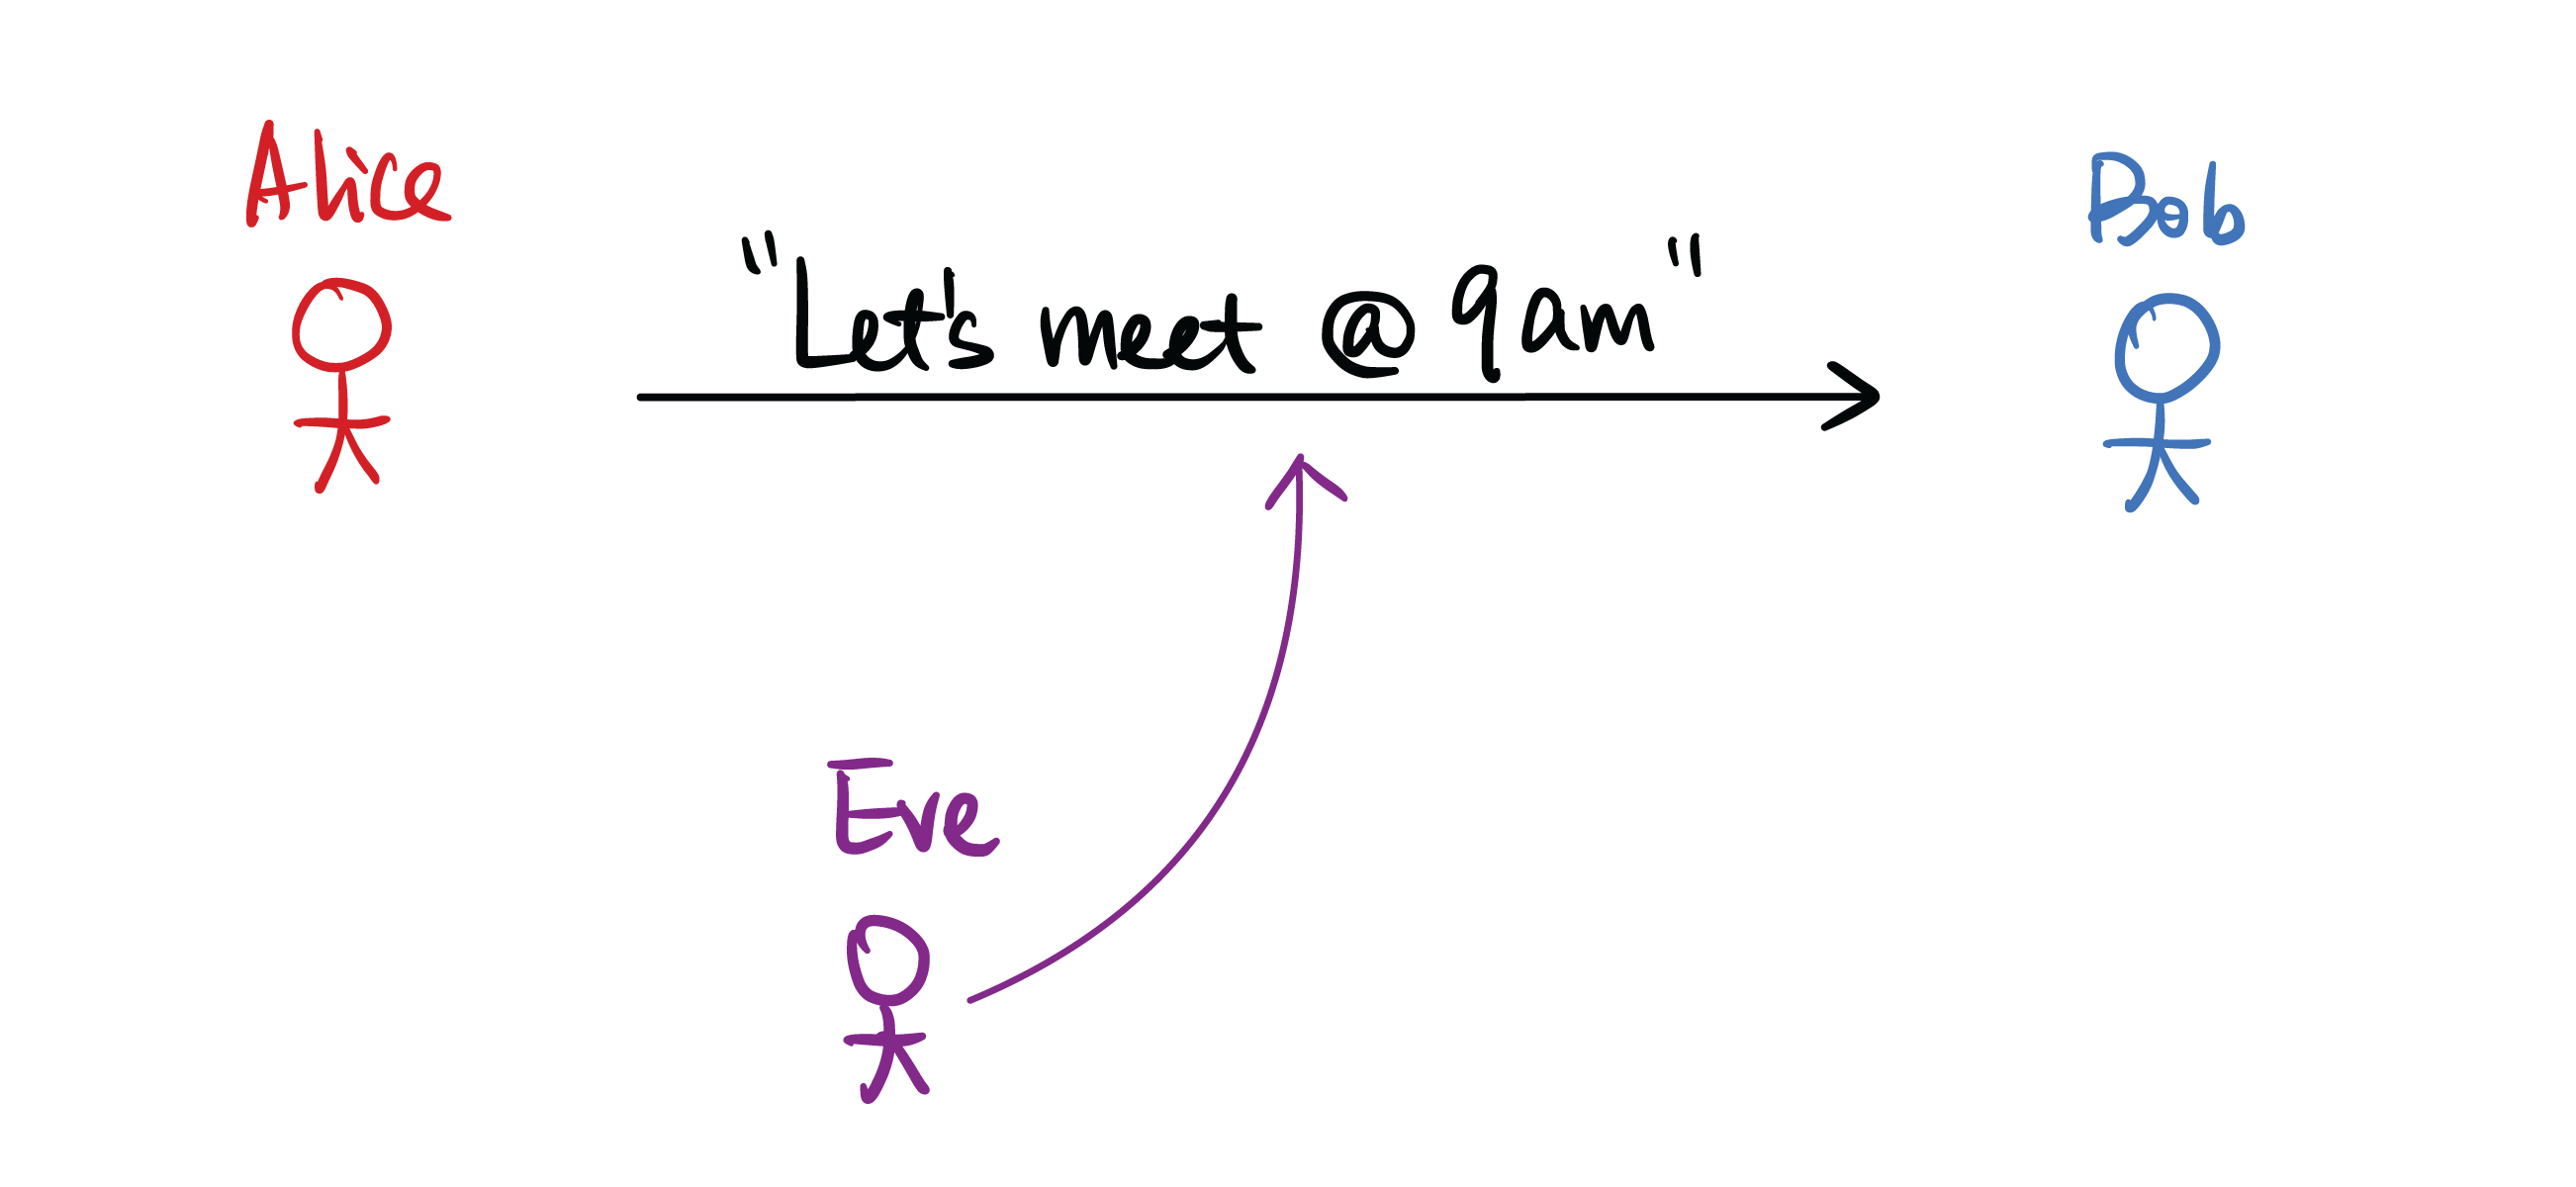
\includegraphics[width=0.8\textwidth]{images/2023-01-26/secure_computation.png}
\end{center}

Assume Alice wants to communicate to Bob ``Let's meet at 9am'', what are some security guarantees we want?

\begin{itemize}
    \item Eve cannot \emph{see} the message from Alice to Bob.
    \item Eve cannot \emph{alter} the message from Alice to Bob.
\end{itemize}

These two guarantees are the most important guarantees! The former is called \ul{message secrecy}, the latter is called \ul{message integrity}.

\subsubsection{Message Secrecy}

\begin{definition}[Message Secrecy]
    We want cryptography to allow Alice to \emph{encrypt} the message $m$ (which we call \emph{plaintext}) by running an algorithm that produces a \emph{ciphertext} $c$.

    Bob will be able to receive the ciphertext $c$ and run a \emph{decrypt} algorithm to produce the message $m$ again. This is akin to a secure box that Alice locks up, and Bob unlocks, while Eve does not know the message.

    \begin{center}
        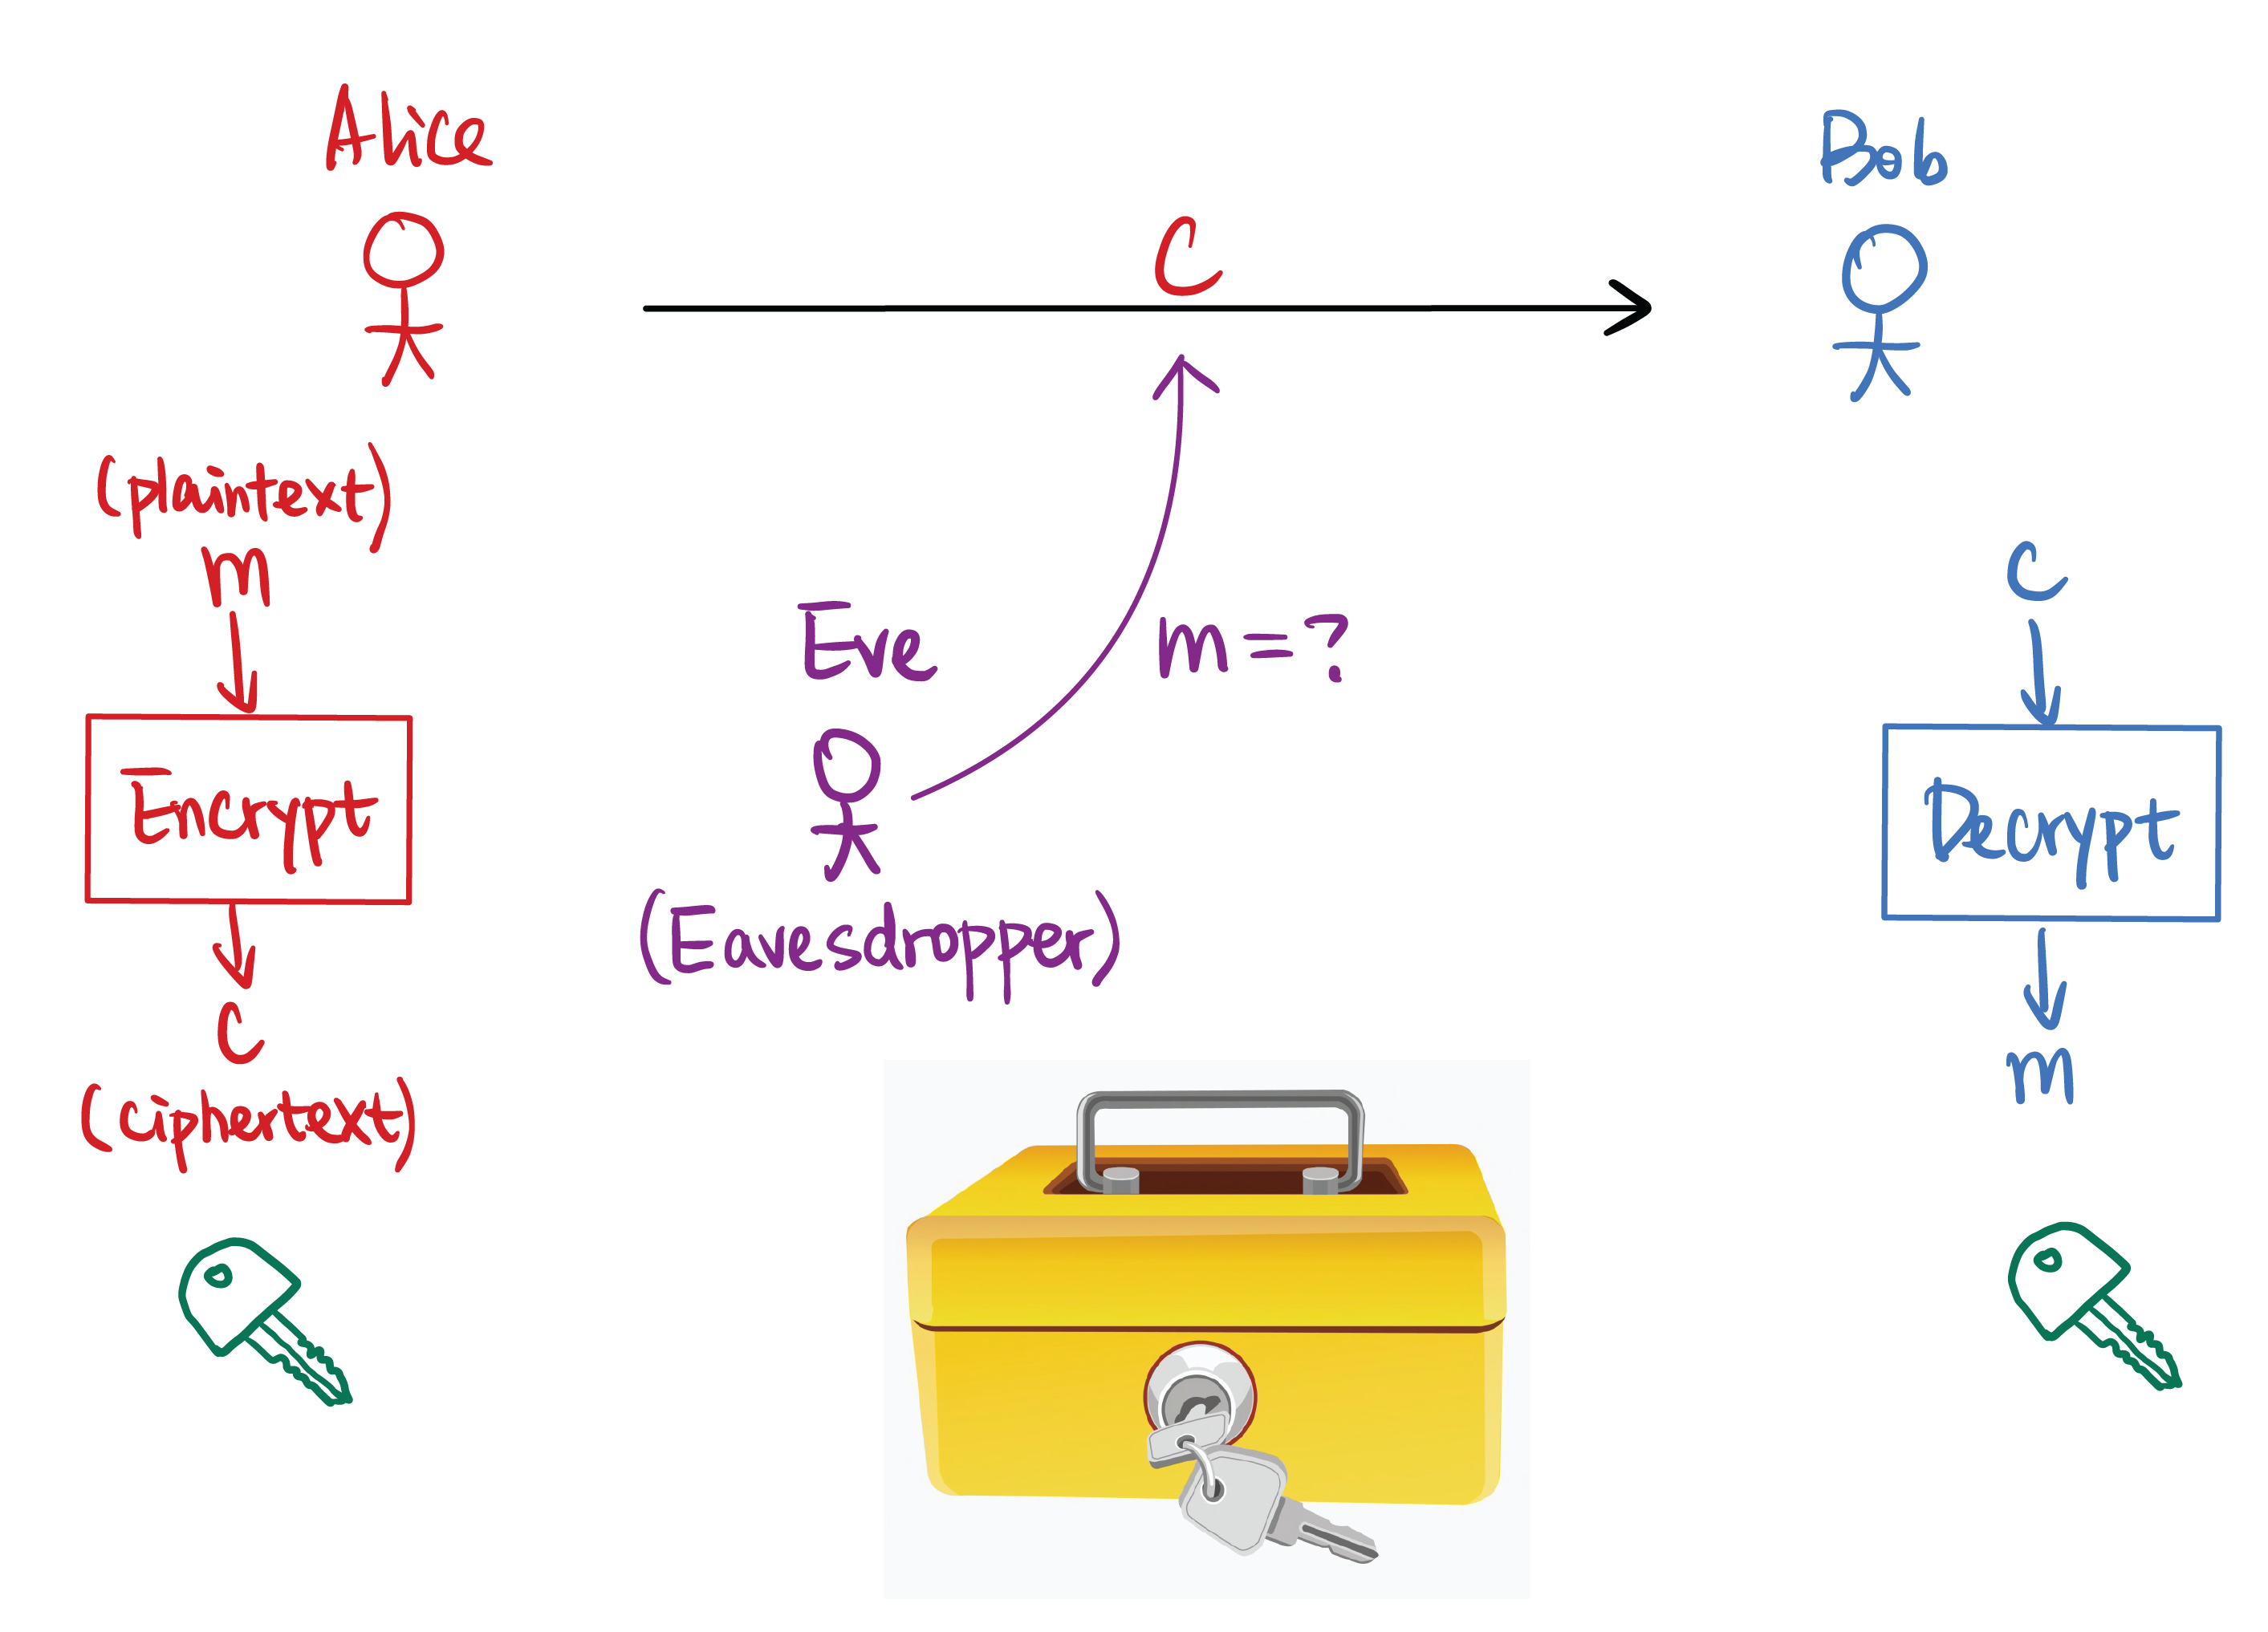
\includegraphics[width=0.8\textwidth]{images/2023-01-26/message_secrecy.png}
    \end{center}

    In this model, Eve is a weaker adversary, an \emph{eavesdropper}. Eve can only see the message, not alter it.
\end{definition}

\begin{example}[Substitution Cipher]
    The key that Alice and Bob jointly uses is a permutation mapping from $\{A\dots Z\}\to \{A\dots Z\}$. This mapping is the \emph{secret key}.

    Bob also has the mapping, and takes the inverse of the permutation to retrieve the message.

    \begin{center}
        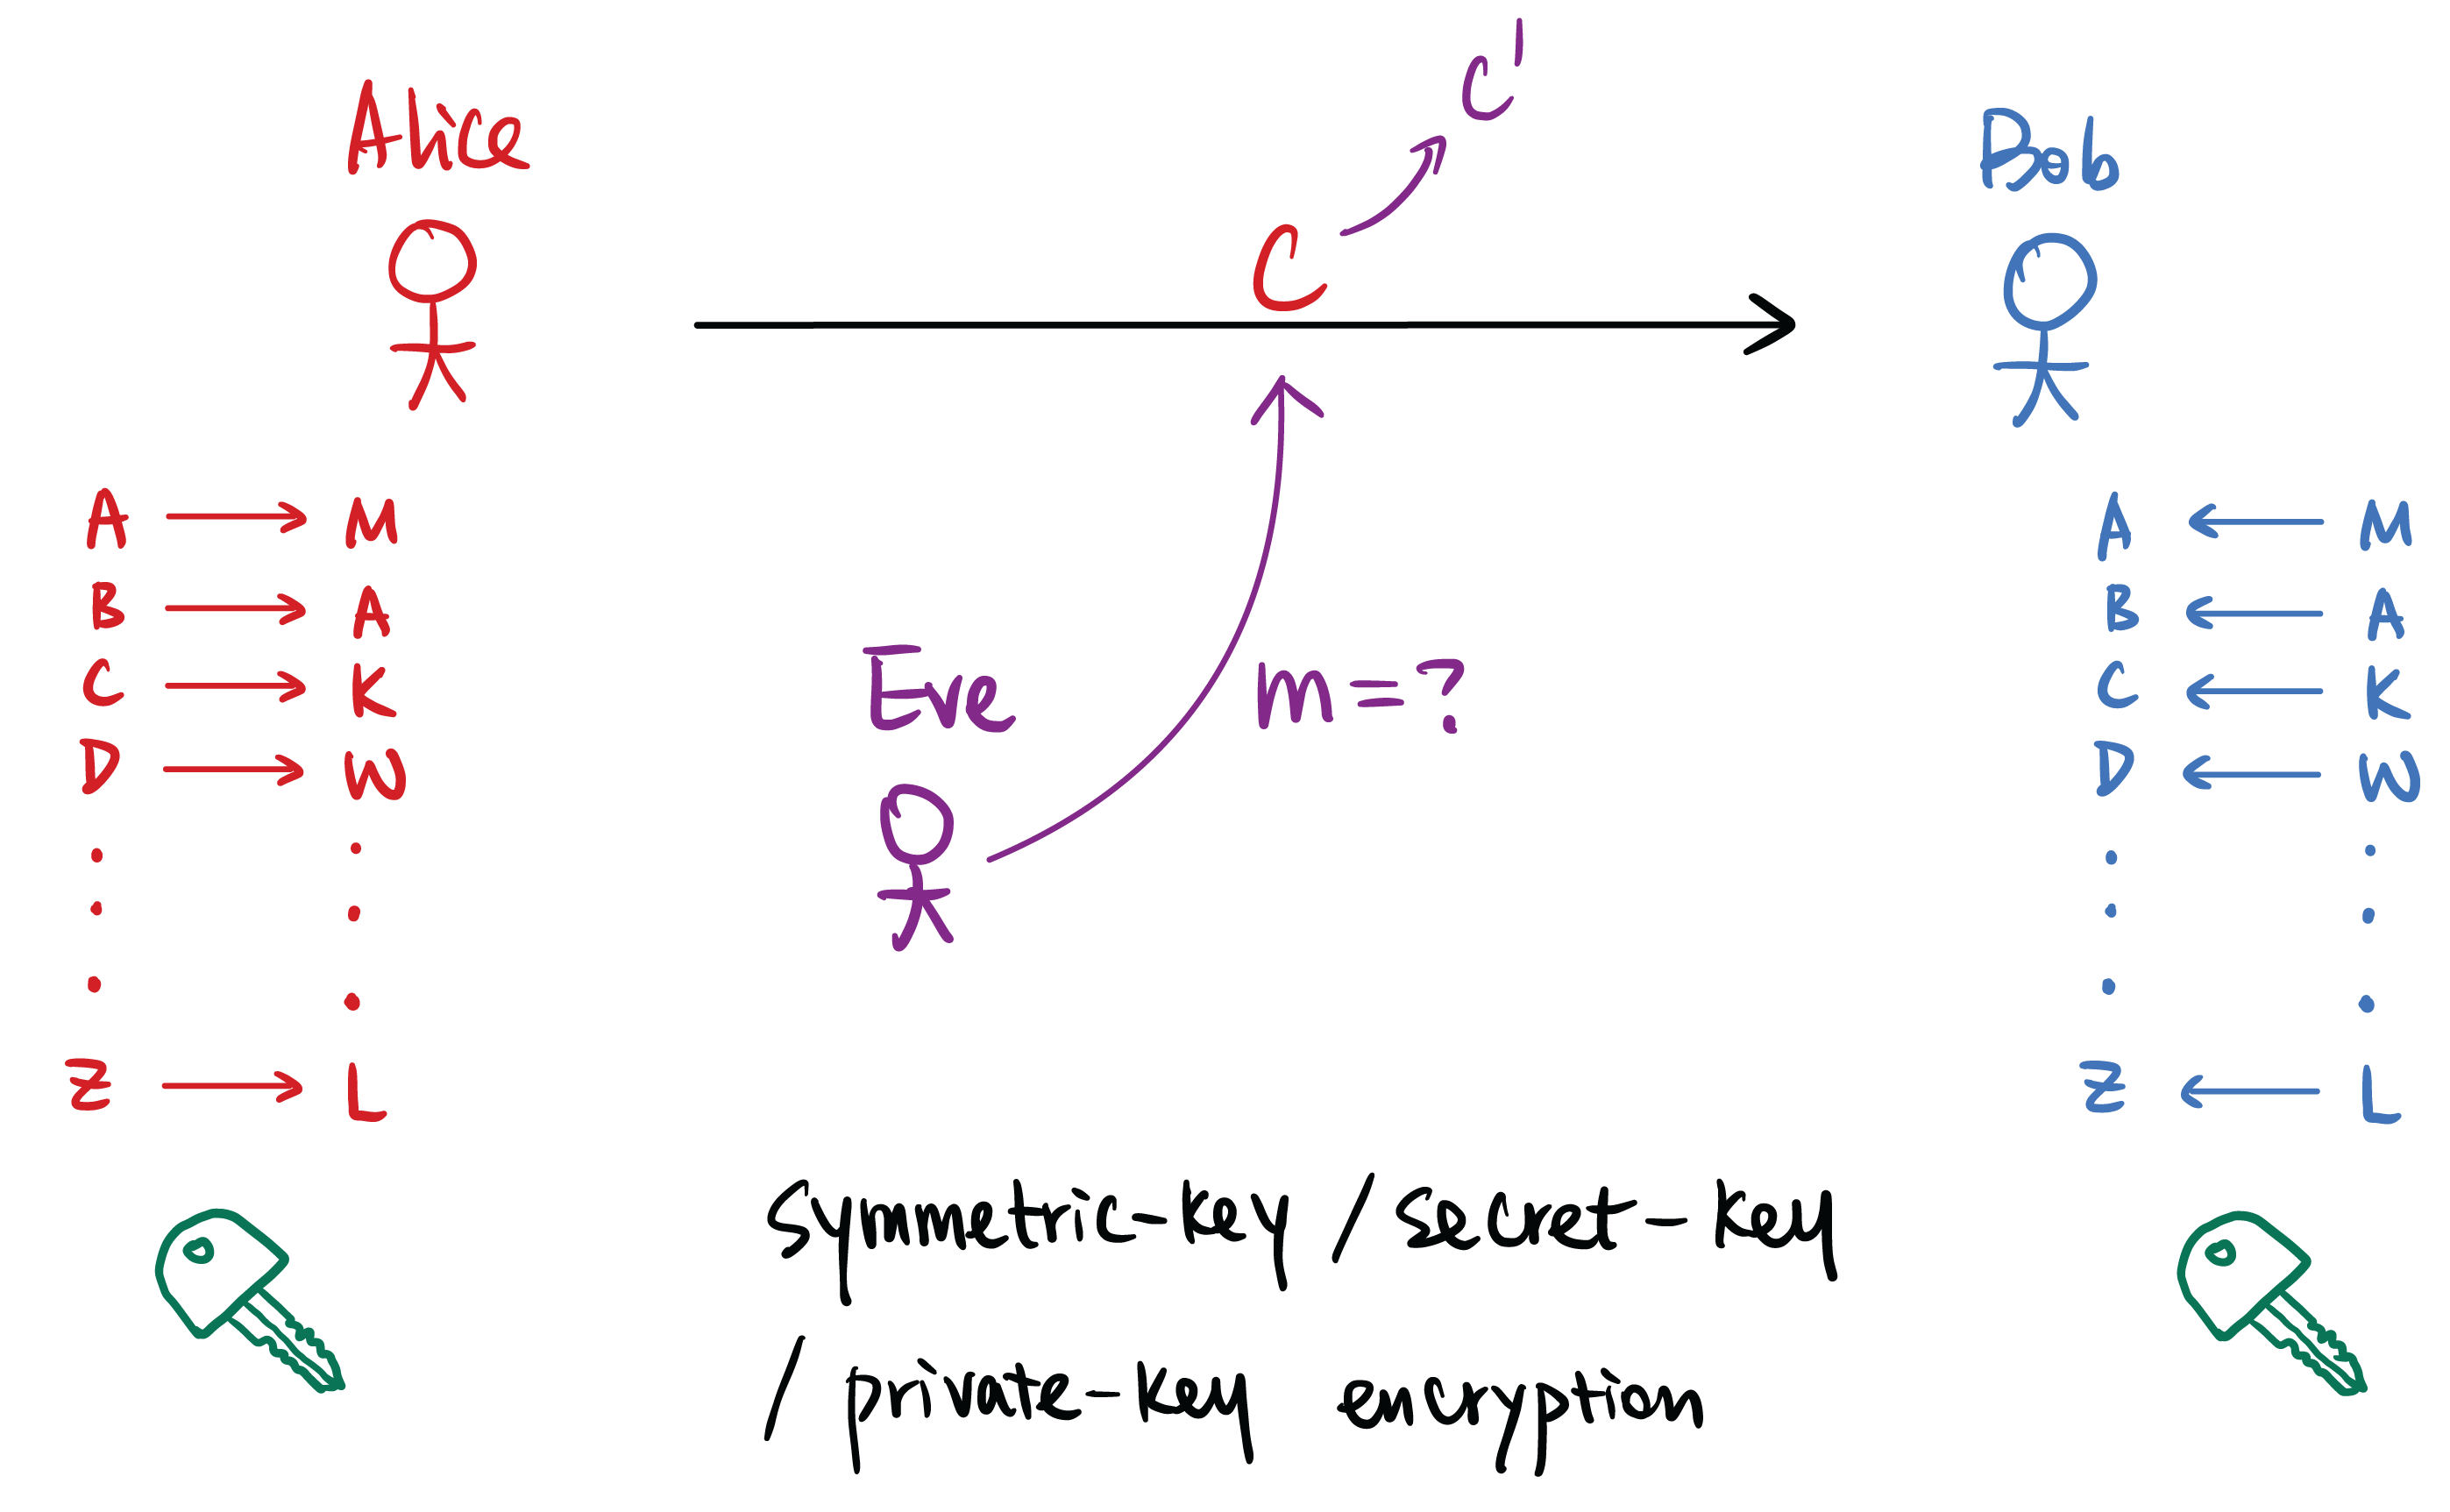
\includegraphics[width=0.9\textwidth]{images/2023-01-26/substitution_cipher.png}
    \end{center}

    This scheme is not quite secure! \emph{Why?}

    You could guess a bunch of vowels and see what words could make up. If you have a long enough message, you can see which letters appear more often. We know that in English, the vowels appear more often; and you can make a lot of guesses.
\end{example}
\begin{remark*}
    This encryption scheme also requires that Alice and Bob meet up in person to exchange this shared private key. Schemes like this are called \emph{symmetric-key, secret-key, or private-key encryption}. They need to meet up first to exchange secret keys.
\end{remark*}

\begin{definition}[Public-key Encryption]
    There is another primitive that is much more ideal/stronger, \ul{public-key encryption}. Bob publishes both a \emph{public} key and a \emph{private} key. You can consider a lock where you don't need a key to lock it\framedfootnote{You literally click it closed}, and only Bob has the key to unlock it.

    \begin{center}
        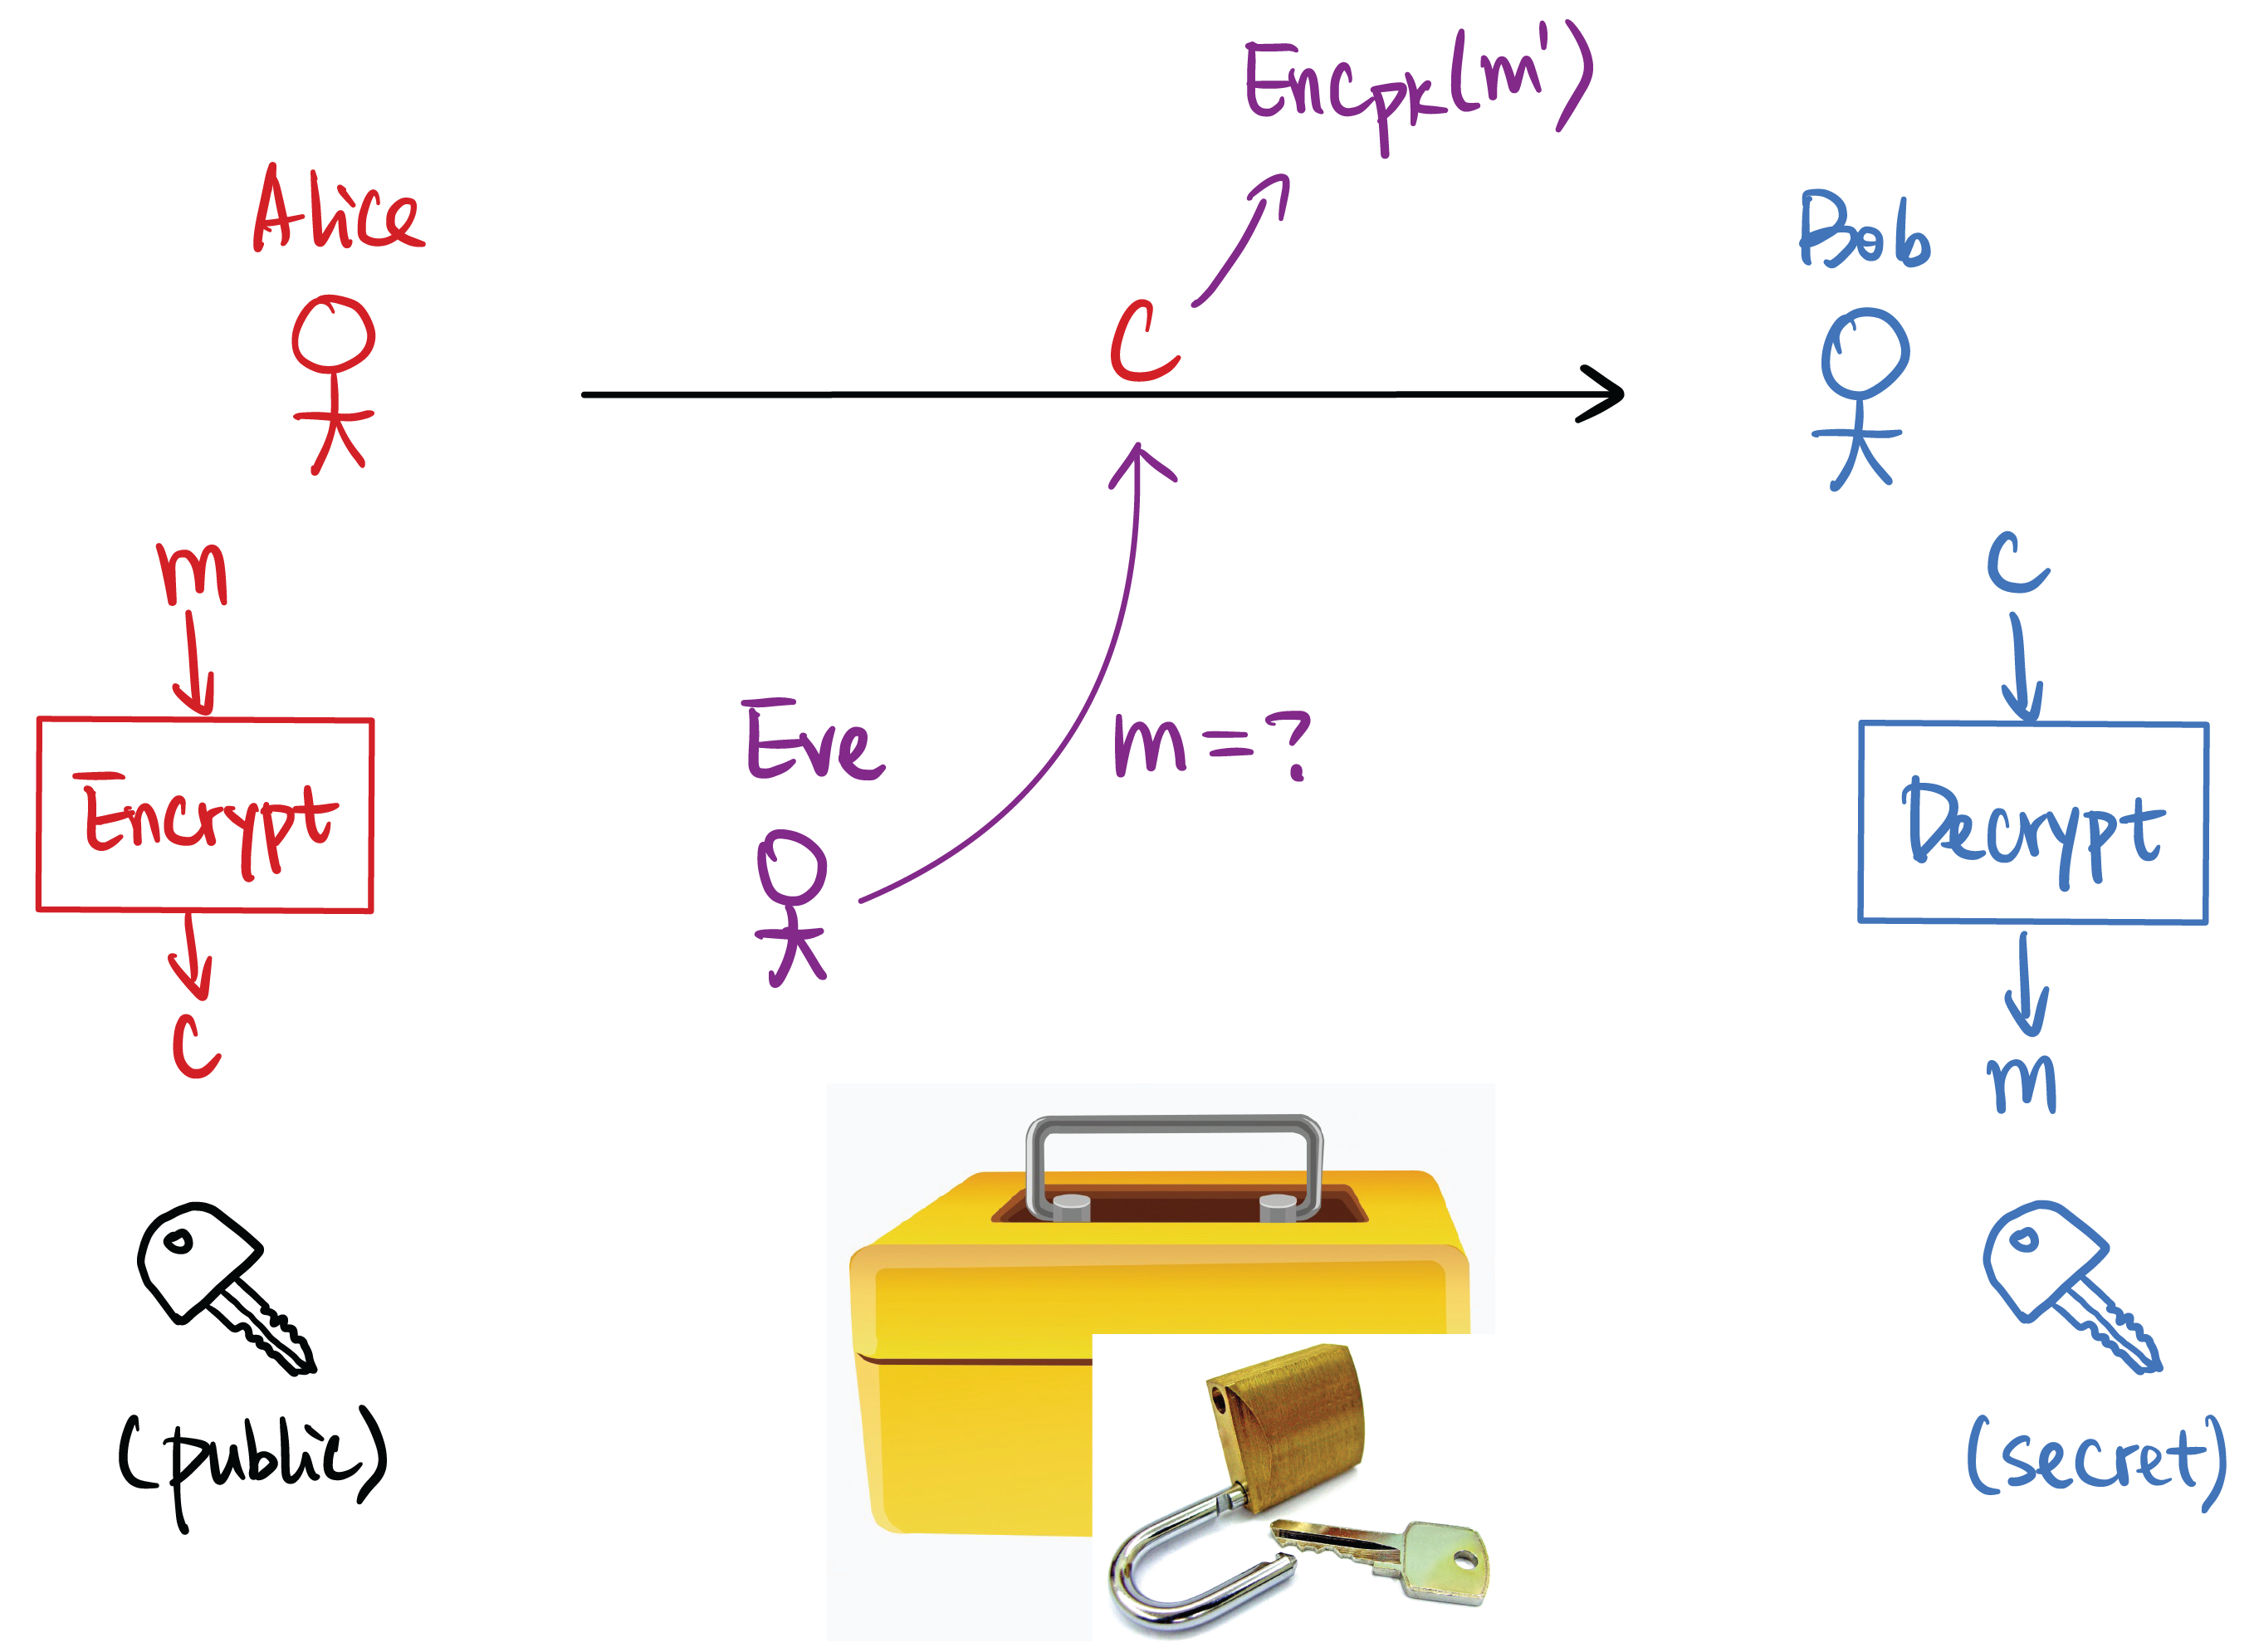
\includegraphics[width=0.9\textwidth]{images/2023-01-26/public_key.png}
    \end{center}

    This is seemingly magic! Bob could publish a public key on his homepage, anyone can encrypt using a public key but only Bob can decrypt. \emph{Stay tuned, we will see public-key encryption schemes next lecture!}
\end{definition}

\subsubsection{Message Integrity}
Alice wants to send a message to Bob again, but Eve is stronger! Eve can now tamper with the message.

\begin{center}
    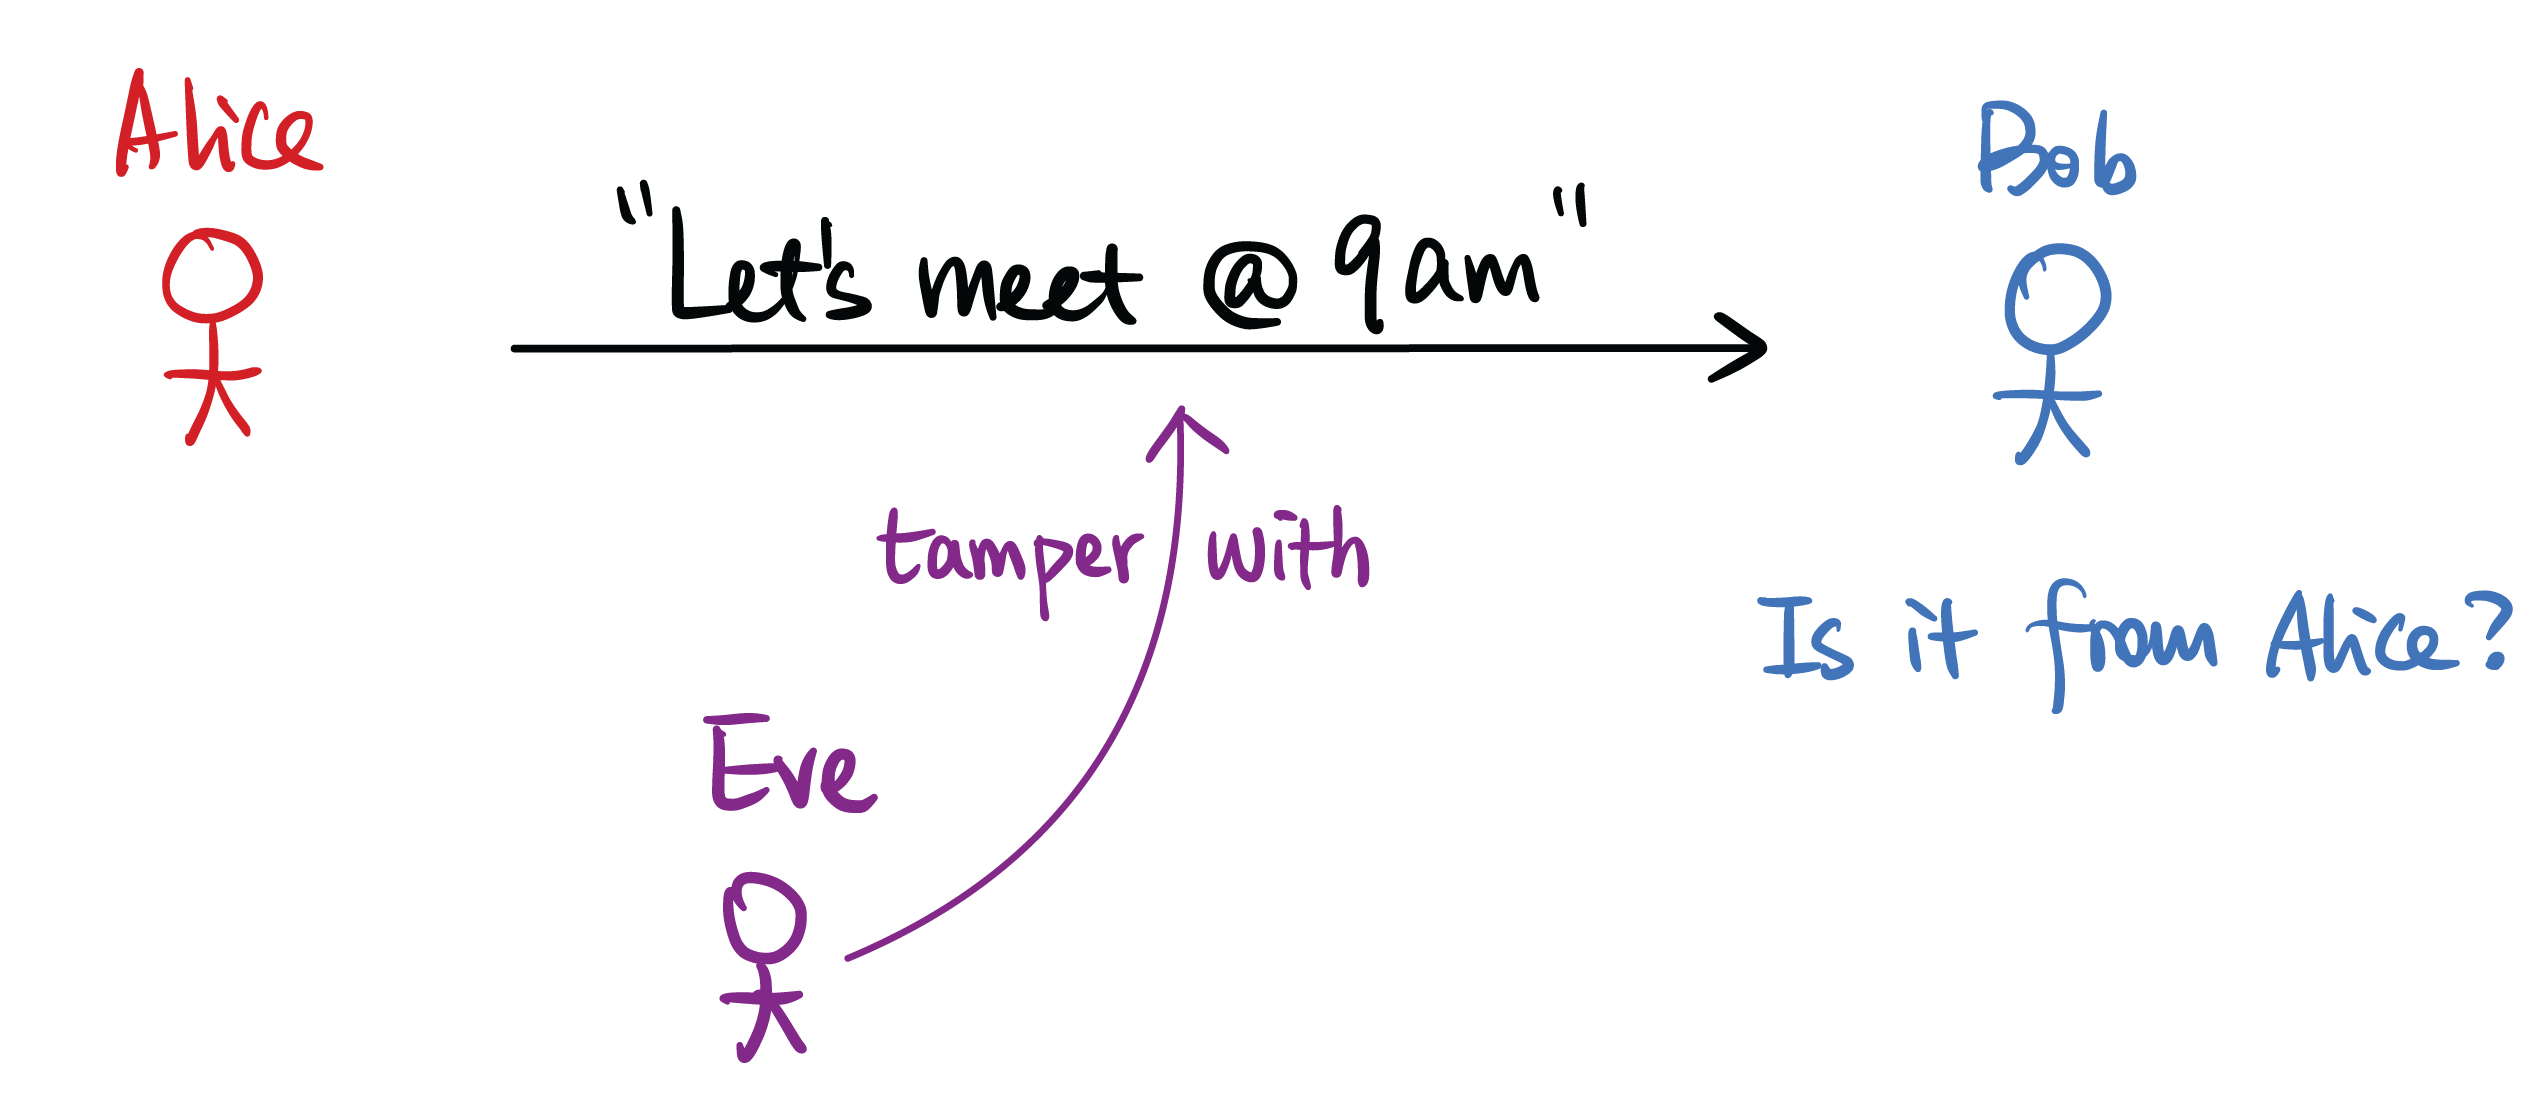
\includegraphics[width=0.9\textwidth]{images/2023-01-26/integrity.png}
\end{center}

Bob wants to ensure that the message \emph{actually} comes from Alice. Does our previous scheme (of encrypting messages) solve this problem? Nope!

Eve can change the ciphertext to something else, they could pretend to be Alice. In secret-key schemes, if Eve figures out the secret-key, they can forge messages from Alice. Even if Eve doesn't know the underlying message, they could still change it to some other ciphertext which might be correlated to the original ciphertext, \emph{without knowing the underlying message}. We'll see how Eve can meaningfully do this in some schemes. Alice could send a message ``Let's meet at $x$ AM'' and Eve could tamper this to say ``Let's meet at $x+1$ AM.''

This is sort of an orthogonal problem to message secrecy. For example, when Alice logs in to Google, Google needs to verify that Alice actually is who she claims to be.

\begin{center}
    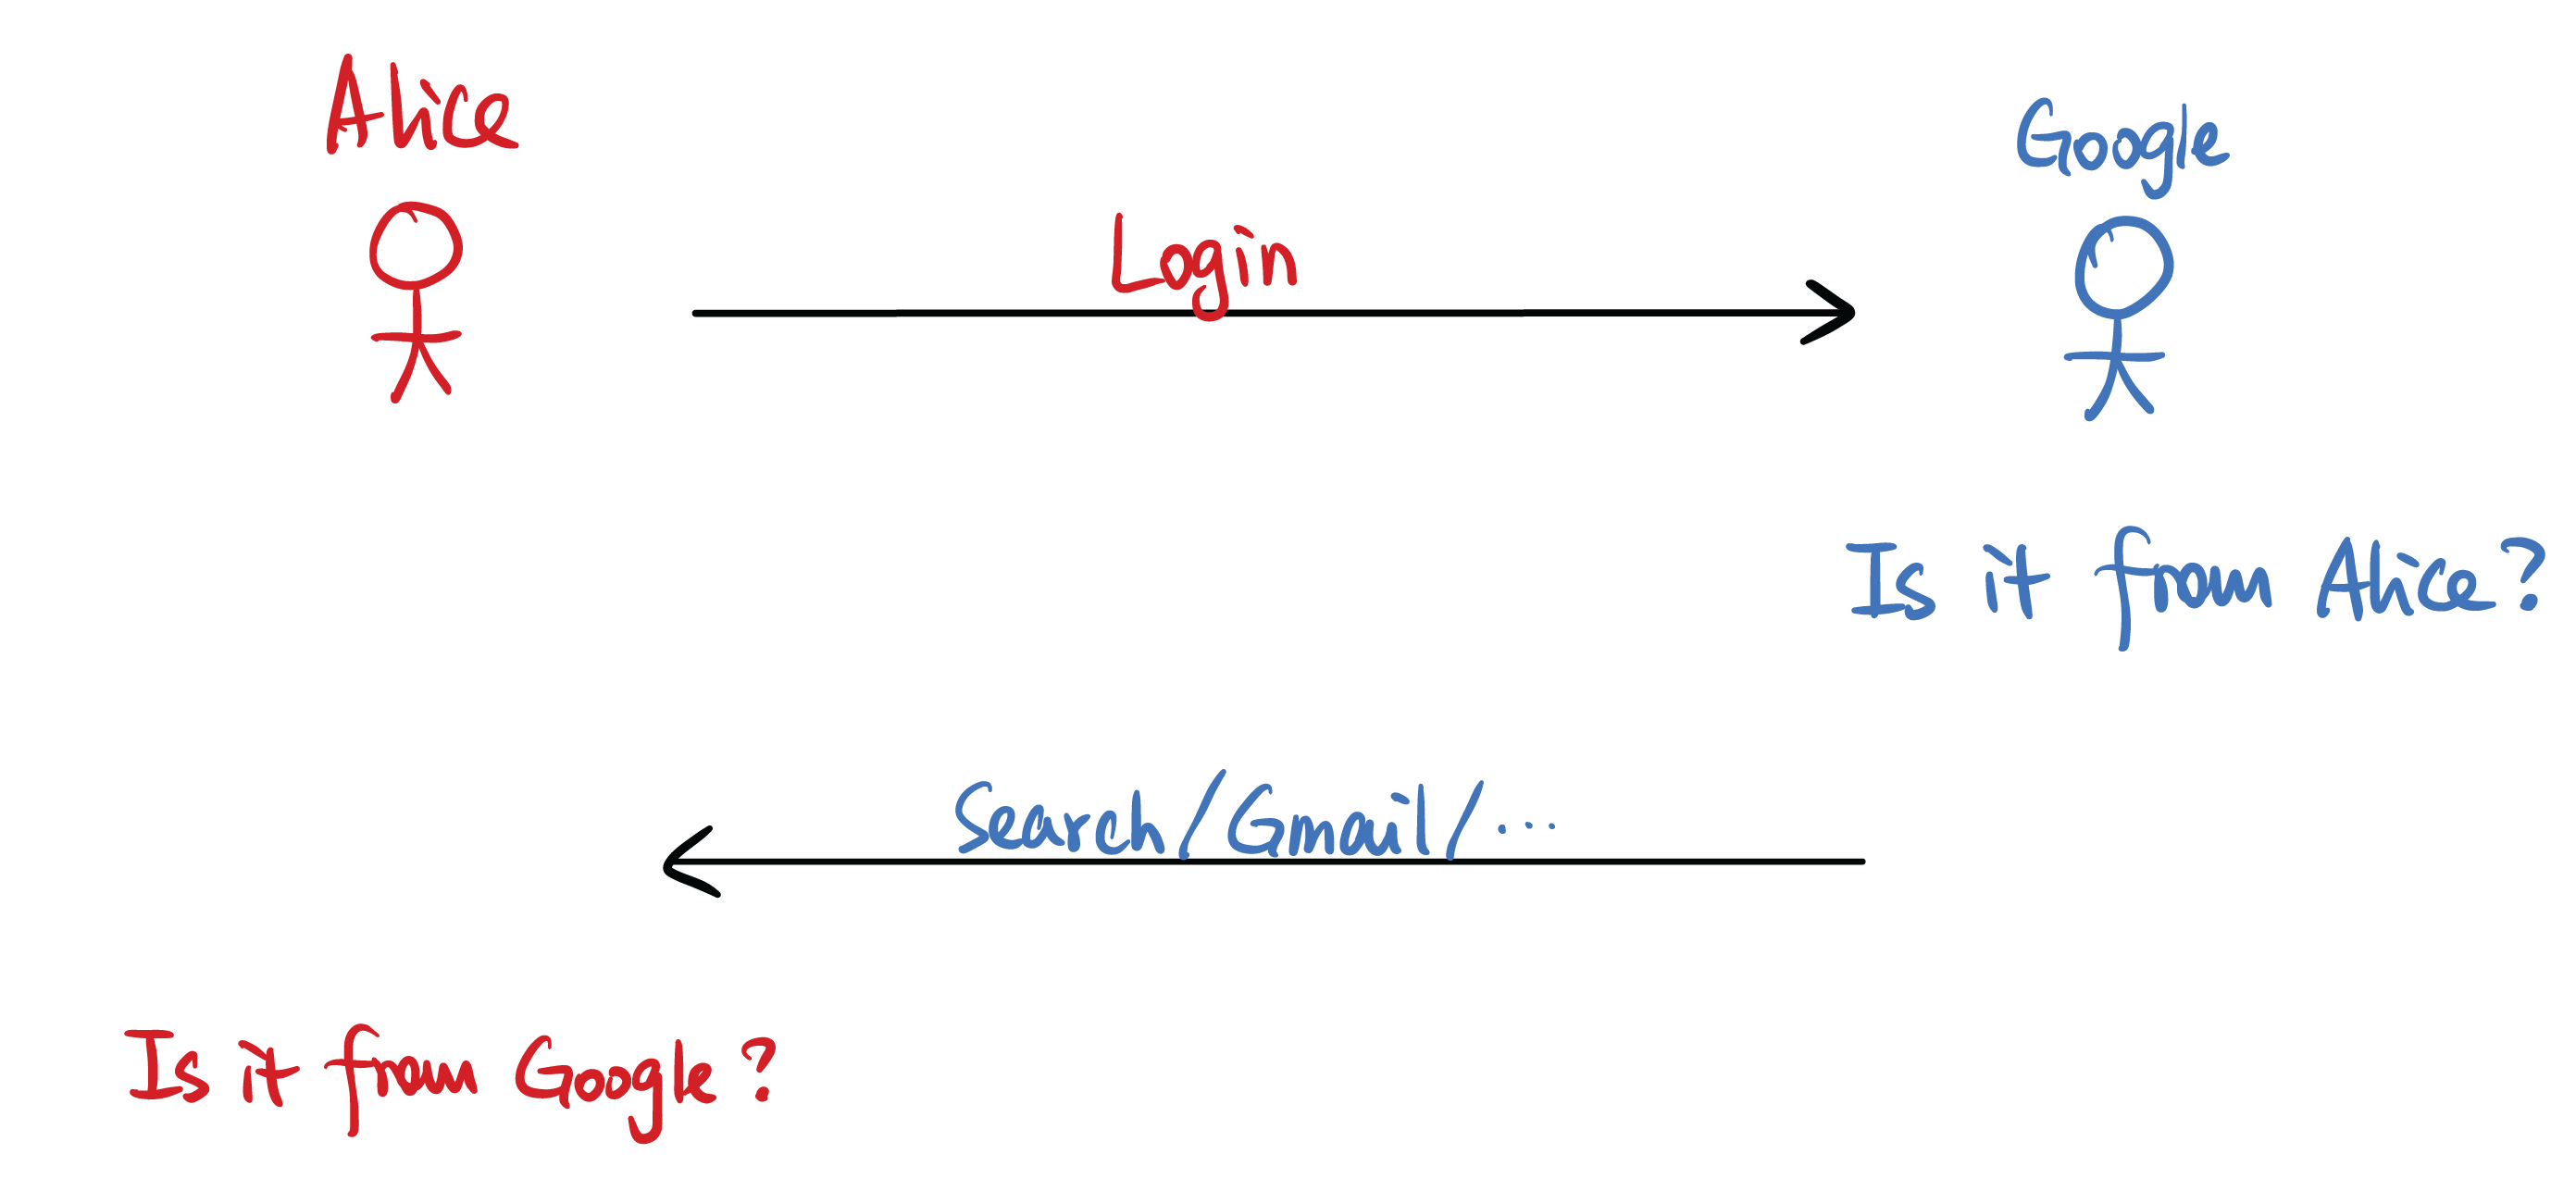
\includegraphics[width=0.9\textwidth]{images/2023-01-26/authentication.png}
\end{center}

\subsection{Project Overview}
\begin{enumerate}
    \setcounter{enumi}{-1}
    \item Warm-up, you will implement some basic cryptographic schemes.
    \item Secure Communication: what was just introduced.
    \item Secure Authentication: how to authenticate yourself to a server, also mentioned just now.
    \item Zero-Knowledge Proofs: we'll use ZKPs to implement a secure voting scheme.
    \item Secure Multiparty Computation: we'll implement a way to run any function securely between two parties.
    \item Fully Homomorphic Encryption: a form of post-quantum cryptography.
\end{enumerate}
We'll quickly introduce the concepts used in the projects.

\subsubsection{Zero-Knowledge Proofs}
This is to prove something without \emph{revealing} any additional knowledge.
\begin{example*}
    Alice claims to be able to differentiate between Coca-Cola and Pepsi! She wants to prove this to Bob without revealing her secrets.

    Bob will randomly sample a bit $b\overset{\$}{\leftarrow}\{0, 1\}$, with $b=0$ being Coca-Cola and $b=1$ being Pepsi. Bob will let Alice taste this drink. Alice will give a guess $b'$ of what drink it is.

    \begin{center}
        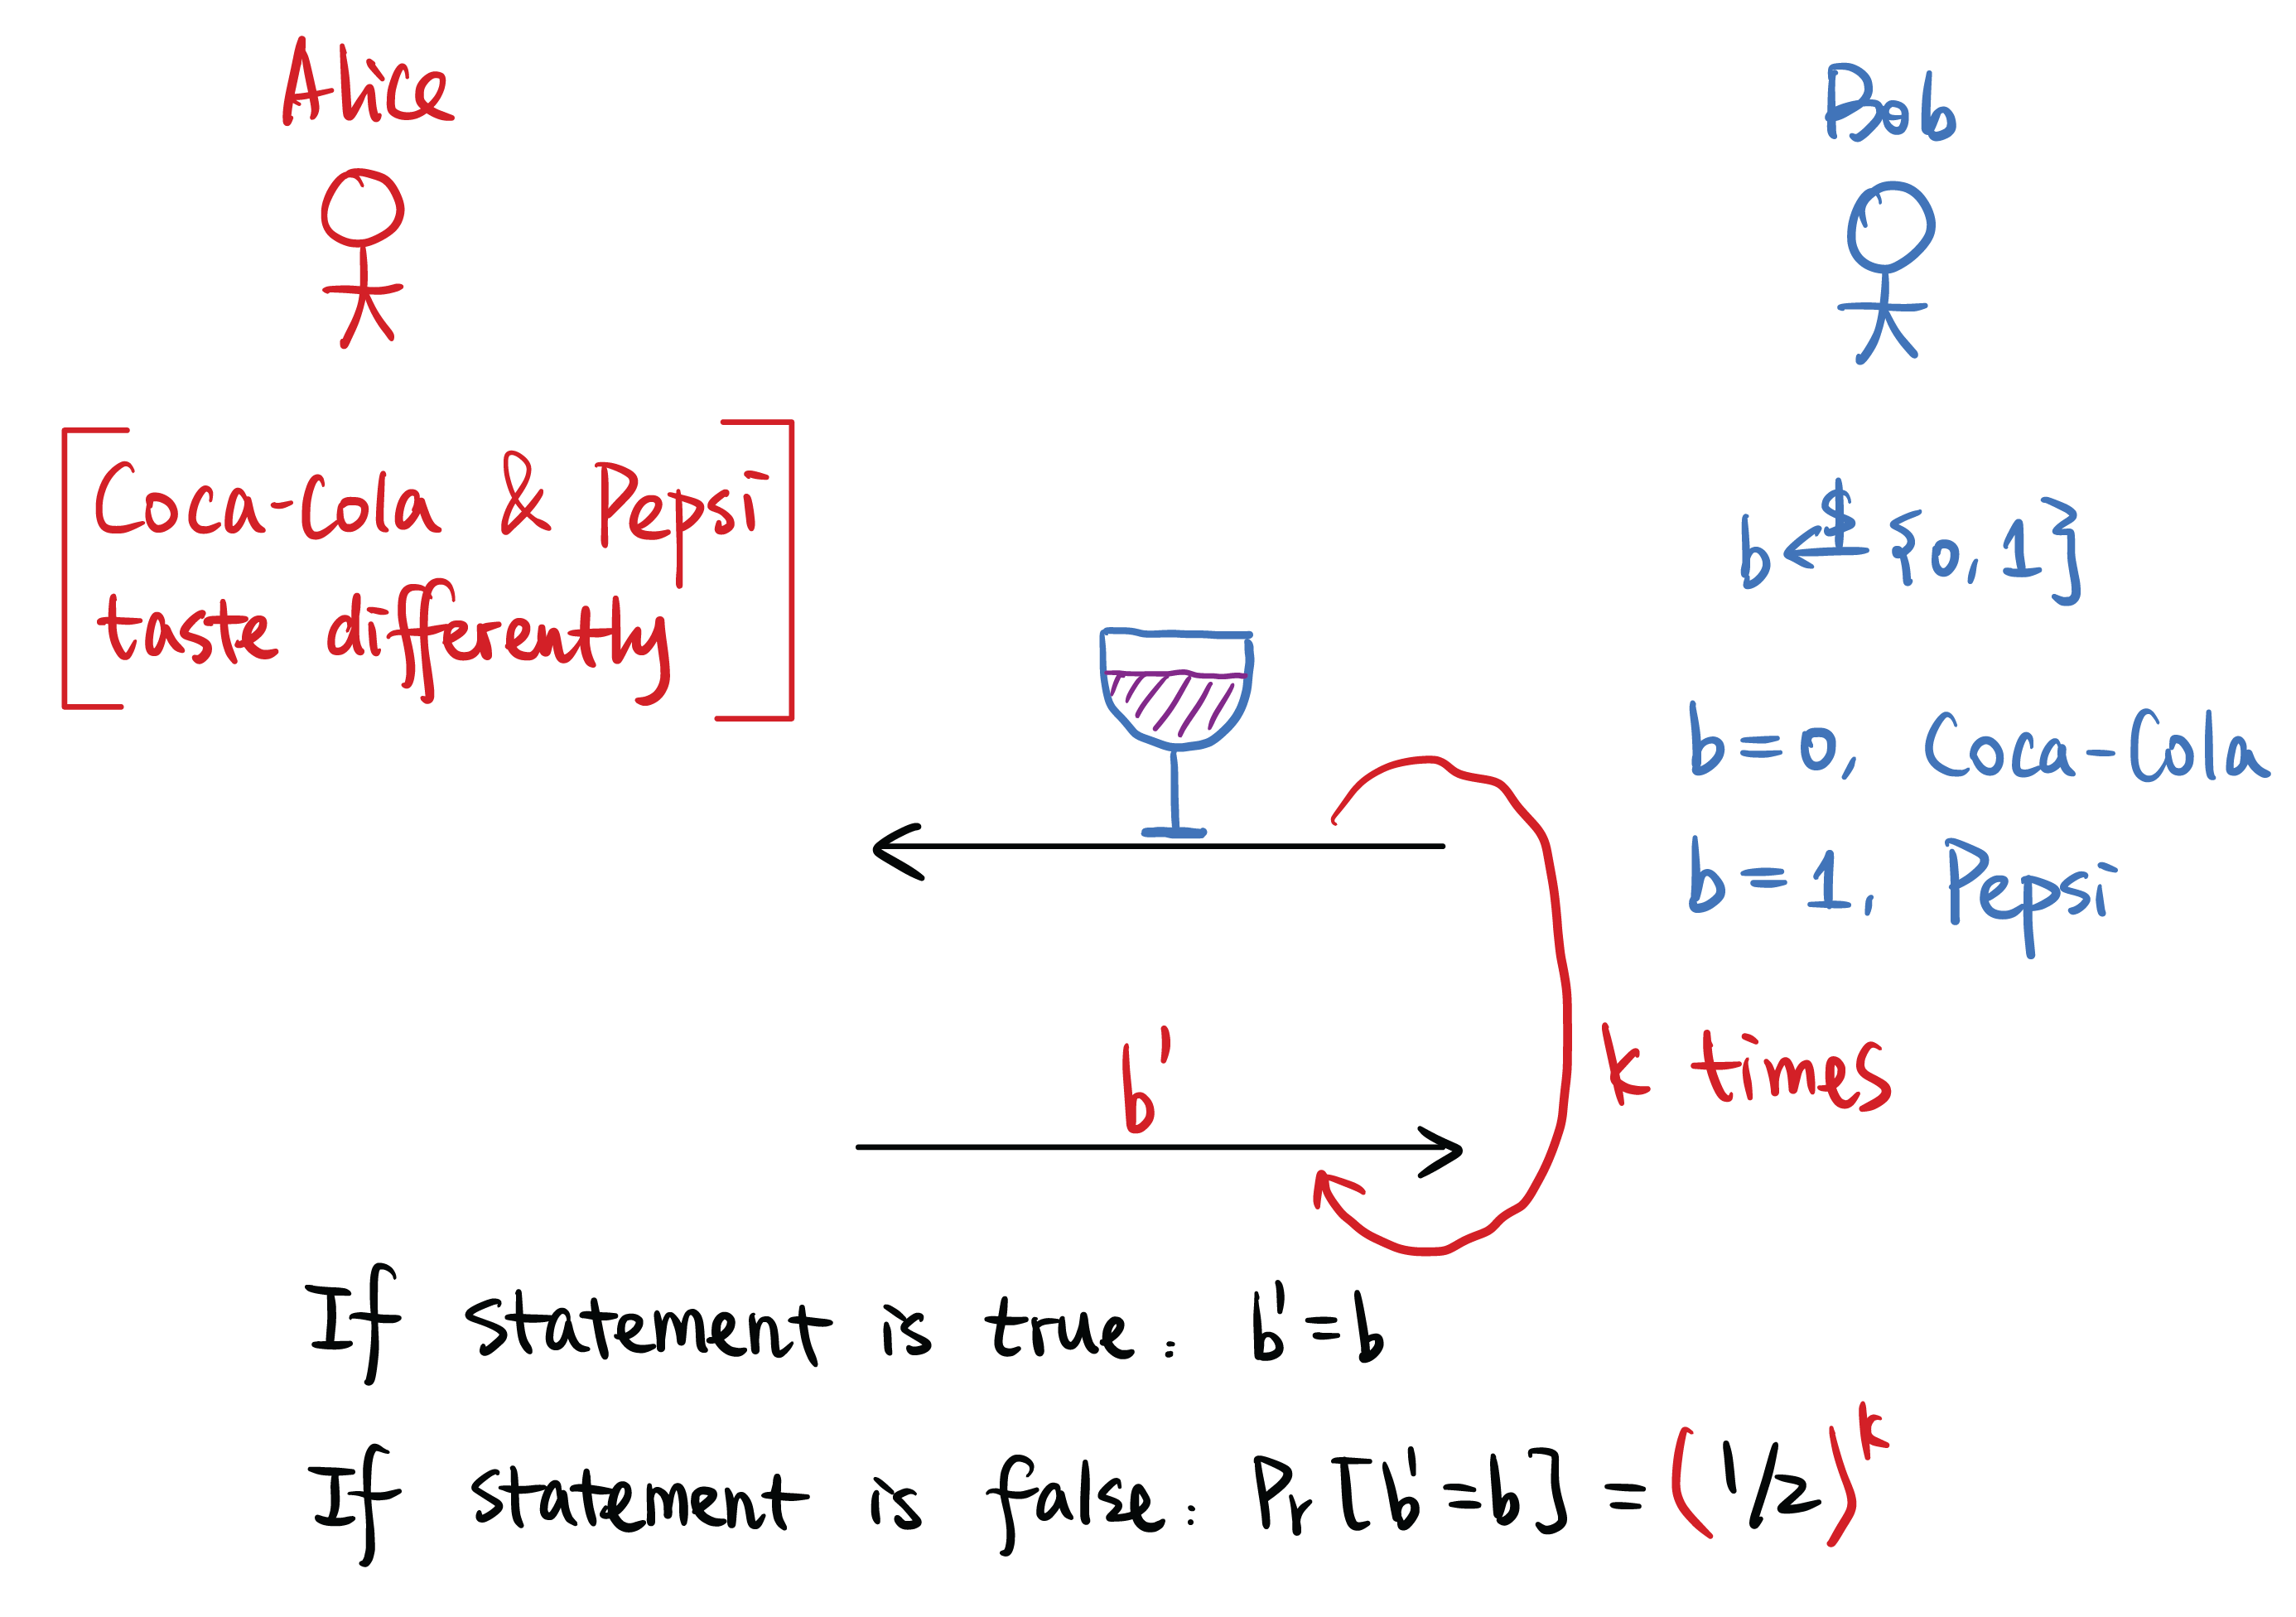
\includegraphics[width=0.9\textwidth]{images/2023-01-26/zk_cola.png}
    \end{center}

    If the statement is true, $b' = b$ (Alice gives the correct prediction).

    If the statement is false, $\Pr[b' = b] = \frac{1}{2}$ (Alice is guessing at $0.5$ probability).

    To enhance this, we can run this a total of $k$ times. If we run it enough times, Bob will be more and more confident in believing this. Alice getting this correct by chance has a $\frac{1}{2^k}$ probability.

    The key idea, however, is that Bob doesn't gain any knowledge of how Alice differentiates.

    \begin{remark*}
        This is a similar strategy in proving graph non-isomorphism.

        For people who have seen this before, generally speaking, any $\textsf{NP}$ language can be proved in zero-knowledge. Alice has the \emph{witness} to the membership in $\textsf{NP}$ language.
    \end{remark*}
\end{example*}

\subsubsection{Secure Multi-Party Computation}
\begin{center}
    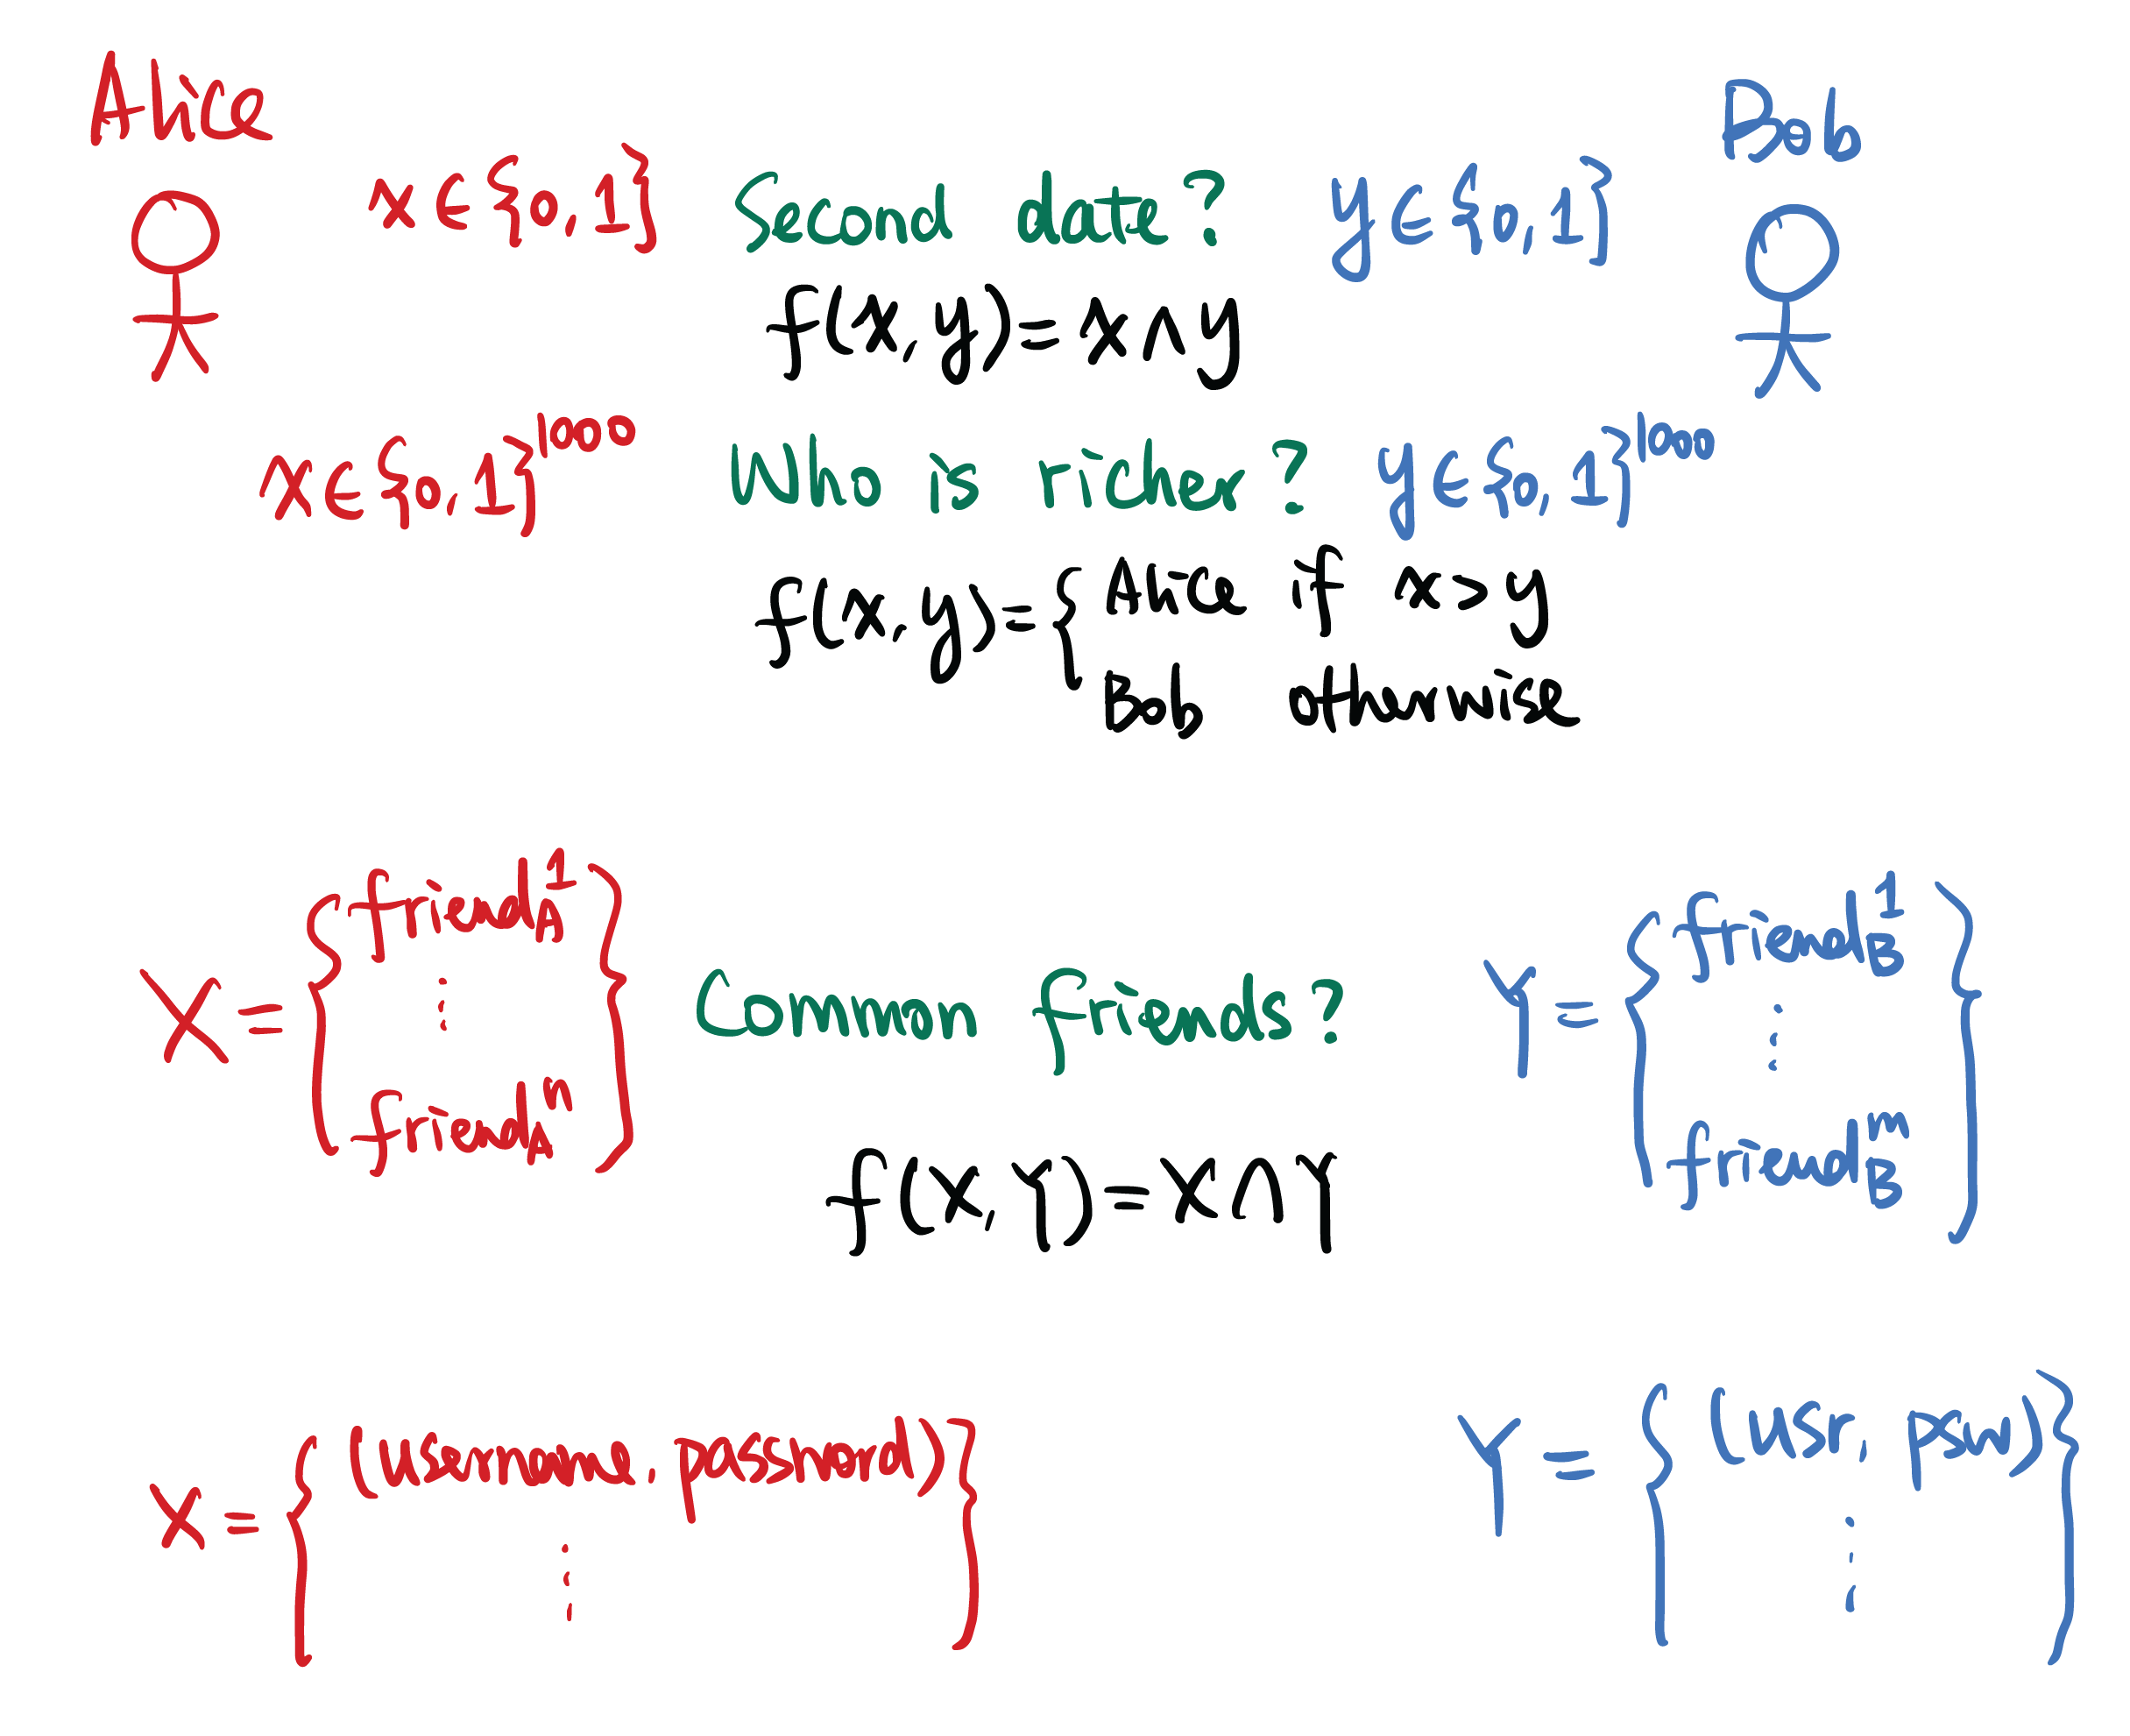
\includegraphics[width=0.9\textwidth]{images/2023-01-26/secure_mpc.png}
\end{center}

\begin{example*}[Secure \textsf{AND}]
    Alice and Bob go on a first date, and they want to figure out whether they want to go on a second date. They will only go on a second date if and only if both agree to a second date.

    How will they agree on this? They could tell each other, but this could be embarrassing. One way is for them to share with a third-party (this is what dating apps do!). However, there might not always be an appropriate third party (in healthcare examples, not everyone can be trusted with the data).

    In this case, Alice has a choice bit $x\in\{0, 1\}$ and Bob has a choice bit $y\in\{0, 1\}$. They are trying to jointly compute $f(x, y) = x\land y$.
\end{example*}

\begin{example*}[Yao's Millionaires' Problem]
    Perhaps, Alice and Bob wants to figure out who is richer. The inputs are $x\in\{0, 1\}^{1000}$ and $y\in\{0, 1\}^{1000}$ (for simplification, let's say they can express their wealth in 1000 bits). The output is the person who has the max.
    \[f(x, y) = \begin{cases}
            \text{Alice} & \text{if }x > y  \\
            \text{Bob}   & \text{otherwise}
        \end{cases}\]
\end{example*}

\begin{example*}[Private Set Intersection]\label{ex:psi}
    Alice and Bob meet for the first time and want to determine which of their friends they share. However, they do not want to reveal who specifically are their friends.

    $X$ is a set of A's friends $X = \{\mathsf{friend}_A^1, \mathsf{friend}_A^2, \cdots, \mathsf{friend}_A^n\}$ and Bob also has a set $Y = \{\mathsf{friend}_B^1, \mathsf{friend}_B^2, \cdots, \mathsf{friend}_B^m\}$. They want to jointly compute \[f(X, Y) = X\cap Y.\]

    You might need to reveal the cardinality of these sets, but you could also pad them up to a maximum number of friends.

    This has a lot of applications in practice! In Google Chrome, your browser will notify you that your password has been leaked on the internet, without having access to your passwords in the clear. $X$ will be a set of \emph{your} passwords, and Google will have a set $Y$ of \emph{leaked} passwords. The \emph{intersection} of these sets are which passwords have been leaked over the internet, without revealing all passwords in the clear.
\end{example*}
\begin{ques*}
    Isn't the assumption that the size is revealed weaker than using a trusted third-party?

    Yes, however in some cases (hospital health records), parties are legally obliged to keep data secure. We wish for security more than the secrecy of cardinality.
\end{ques*}

In the general case, Alice and Bob have some inputs $x$ and $y$ with bounded length, and they want to jointly compute some function $f$ on these inputs. This is \ul{Secure Two-Party Computation}. Furthermore, there could be multiple parties $x_1, \dots, x_n$ that jointly compute $f(x_1, \dots, x_n)$ that hides each input. This is \ul{Secure Multiparty Computation}.

We'll explore a toy example with the bit-\textsf{AND} from the dating example.

\begin{example*}[Private Dating]
    Alice and Bob have choice bits $x\in\{0, 1\}$ and $y\in\{0, 1\}$ respectively. There is a \emph{physical} round table with $5$ identical slots, one already filled in with a $1$ facing down.

    \begin{center}
        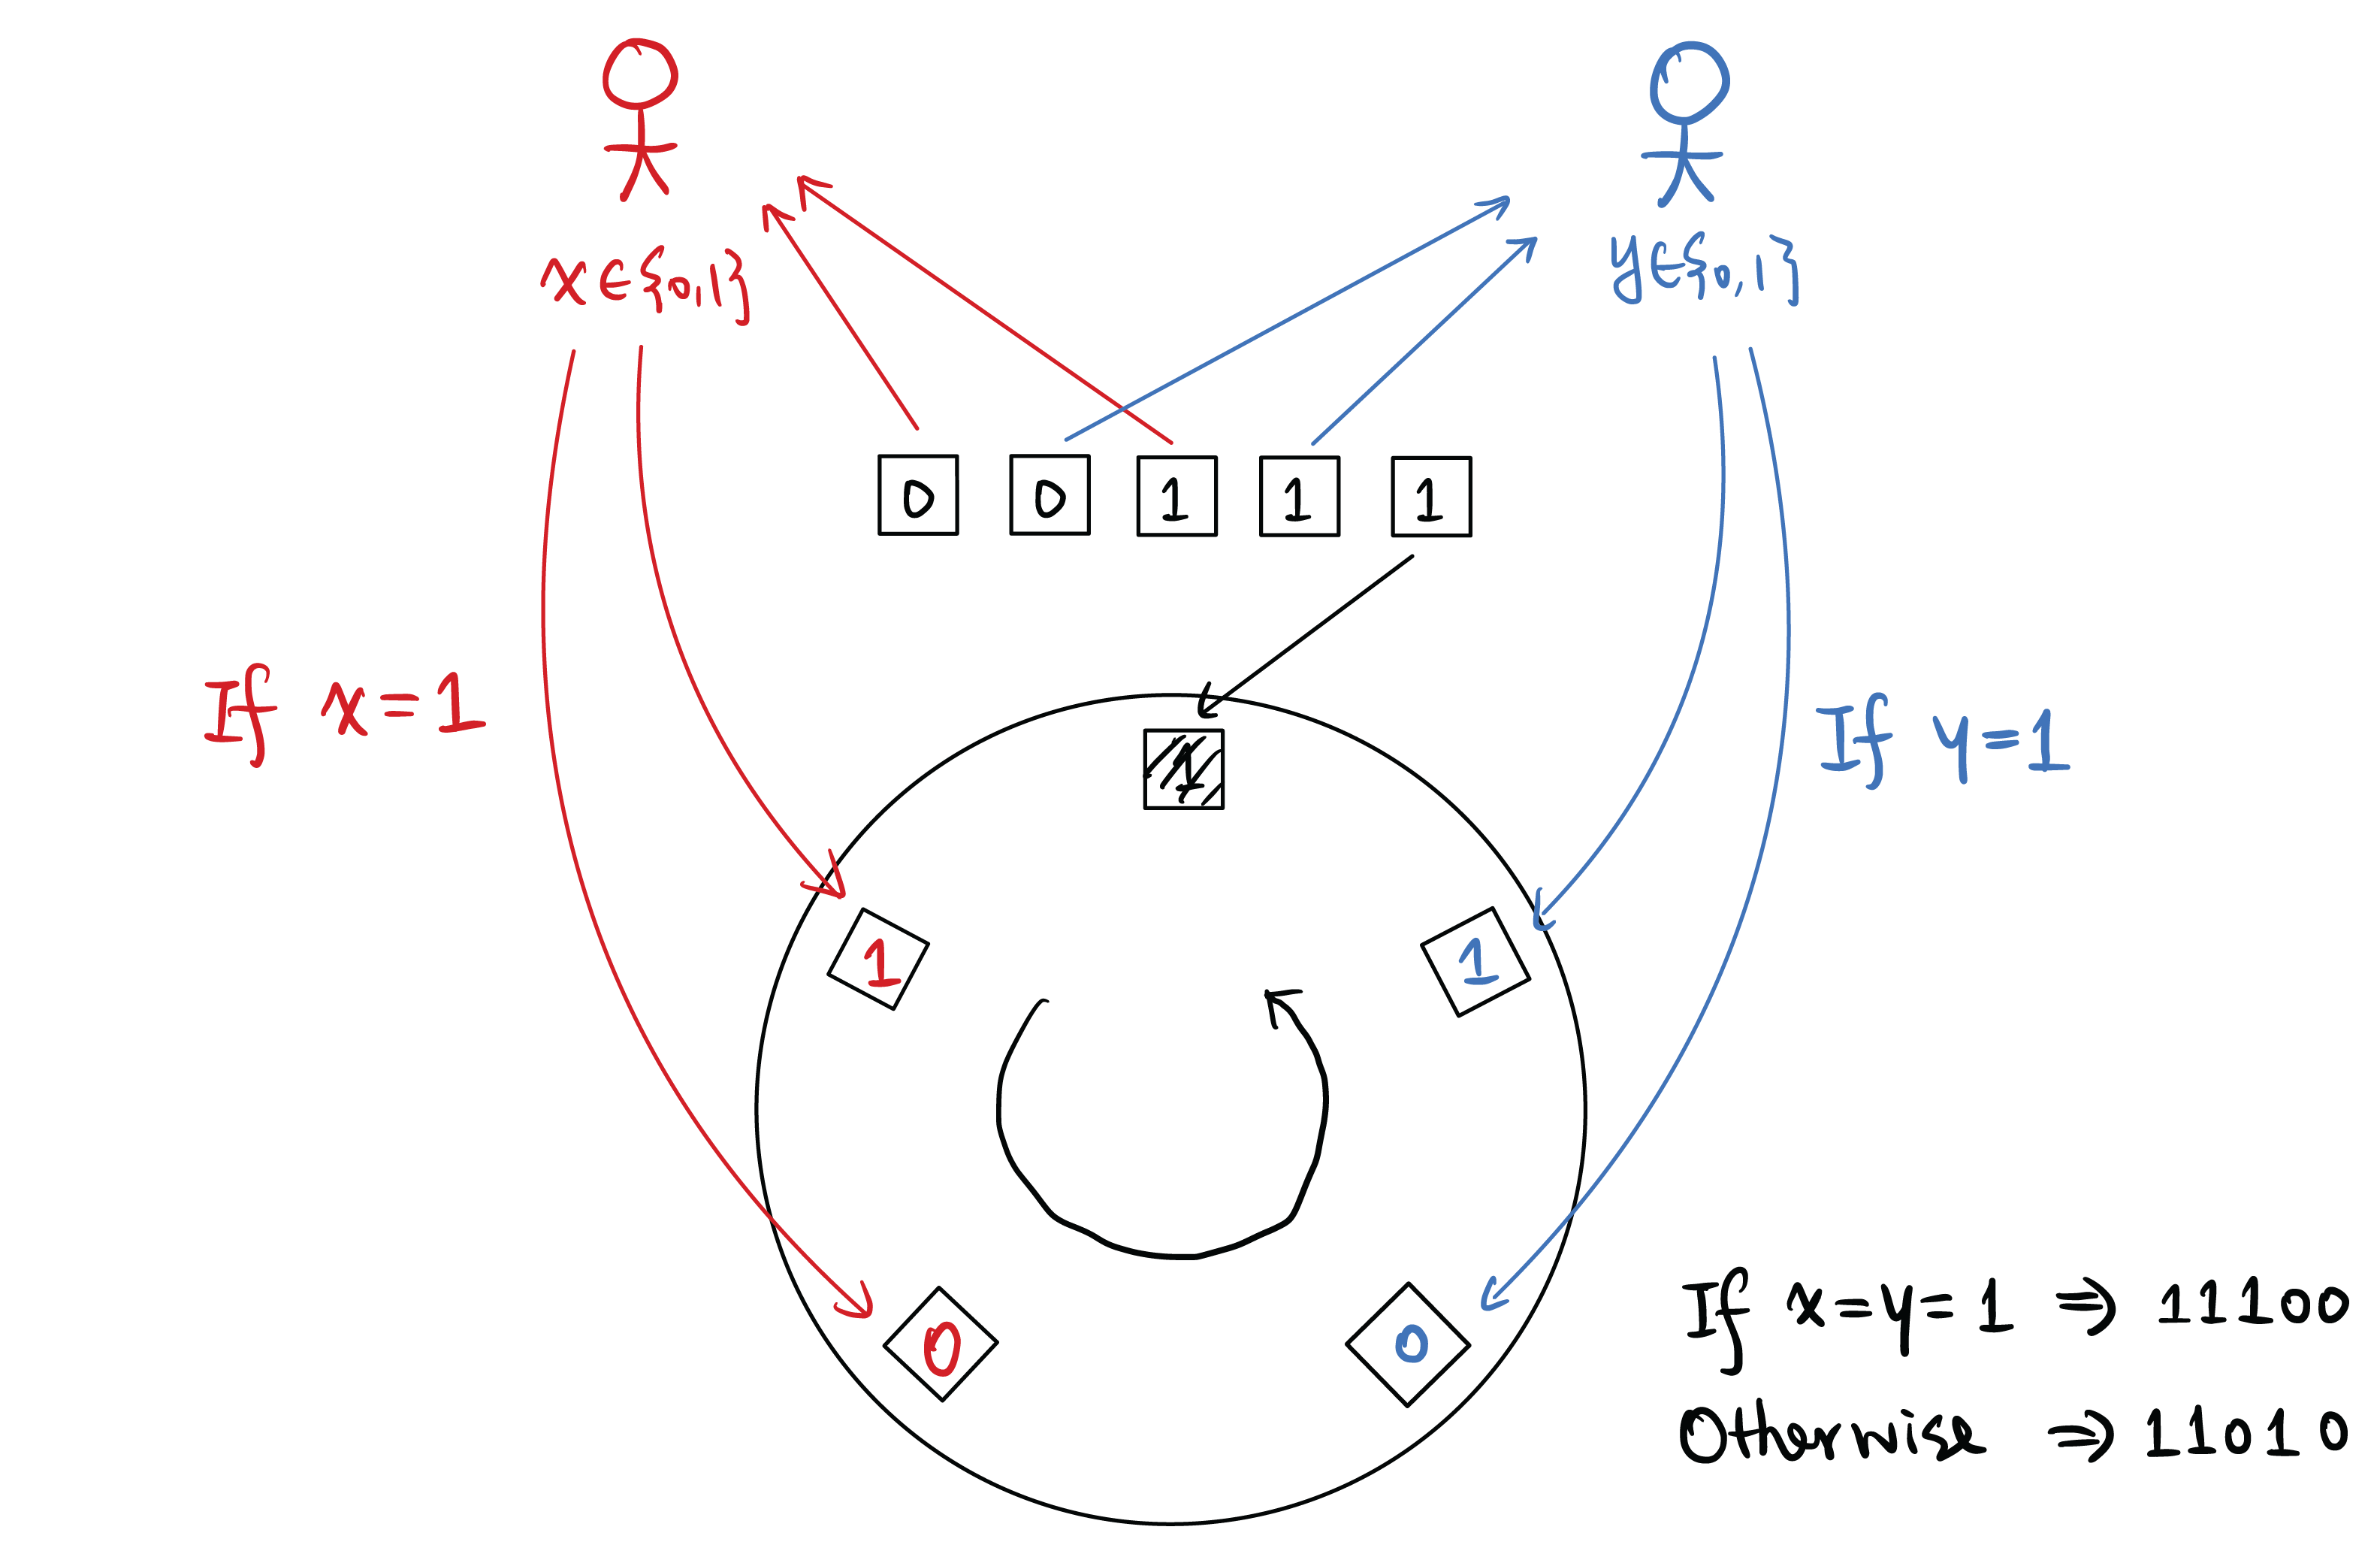
\includegraphics[width=0.9\textwidth]{images/2023-01-26/private_dating.png}
    \end{center}

    Alice and Bob each have identical $0, 1$ cards (each of the $0$ and $1$ cards are indistinguishable from cards of the same value). Alice places her cards on the 2 slots in some order, and Bob does the same.

    They then spin the table around and reveal all the cards, learning $x\land y$.

    If $x = 1$, Alice places it as $1$ on top of $0$, and if $y = 1$, Bob places it as $1$ on top of $0$ as well. Otherwise, they flip them. If $x = y = 1$, then the $0$'s will be adjacent. If $x \neq y$, the order will be $1,1,0,1,0$ (the $0$'s are not adjacent), regardless of which of Alice or Bob produced $x = 0$ (or both!).
\end{example*}
\begin{ques*}
    If Alice puts $1$, and the output is $0$, she could infer the information from Bob. However, this is allowed. Whatever can be inferred from the desired output is inferred.

    The more sensitive part is when if you put a $0$, you don't learn whether the other party also put down a $0$.
\end{ques*}
\emph{This is a toy example! It doesn't use cryptography at all! Two parties have to sit in front of a table. This is called card-based cryptography. We will be using more secure primitives.}

\subsubsection{Fully Homomorphic Encryption}
We'll come back to the secure messaging example.

Alice wants to send Bob a message. She encrypts it somehow and sends a ciphertext $c_1 = \mathsf{Enc}(m_1)$. A nice feature for some encryption schemes is for Eve to do some computation homomorphically on the ciphertexts. Eve might possibly want to add ciphertexts (that leads to plaintext adding)
\[c_1 = \mathsf{Enc}(m_1), c_2 = \mathsf{Enc}(m_2)\Rightarrow c' = \mathsf{Enc}(m_1 + m_2)\]
or perhaps $c'' = \mathsf{Enc}(m_1\cdot m_2)$, or compute arbitrary functions. \emph{Sometimes}, this is simply adding $c_1 + c_2$, but usually not.

\begin{center}
    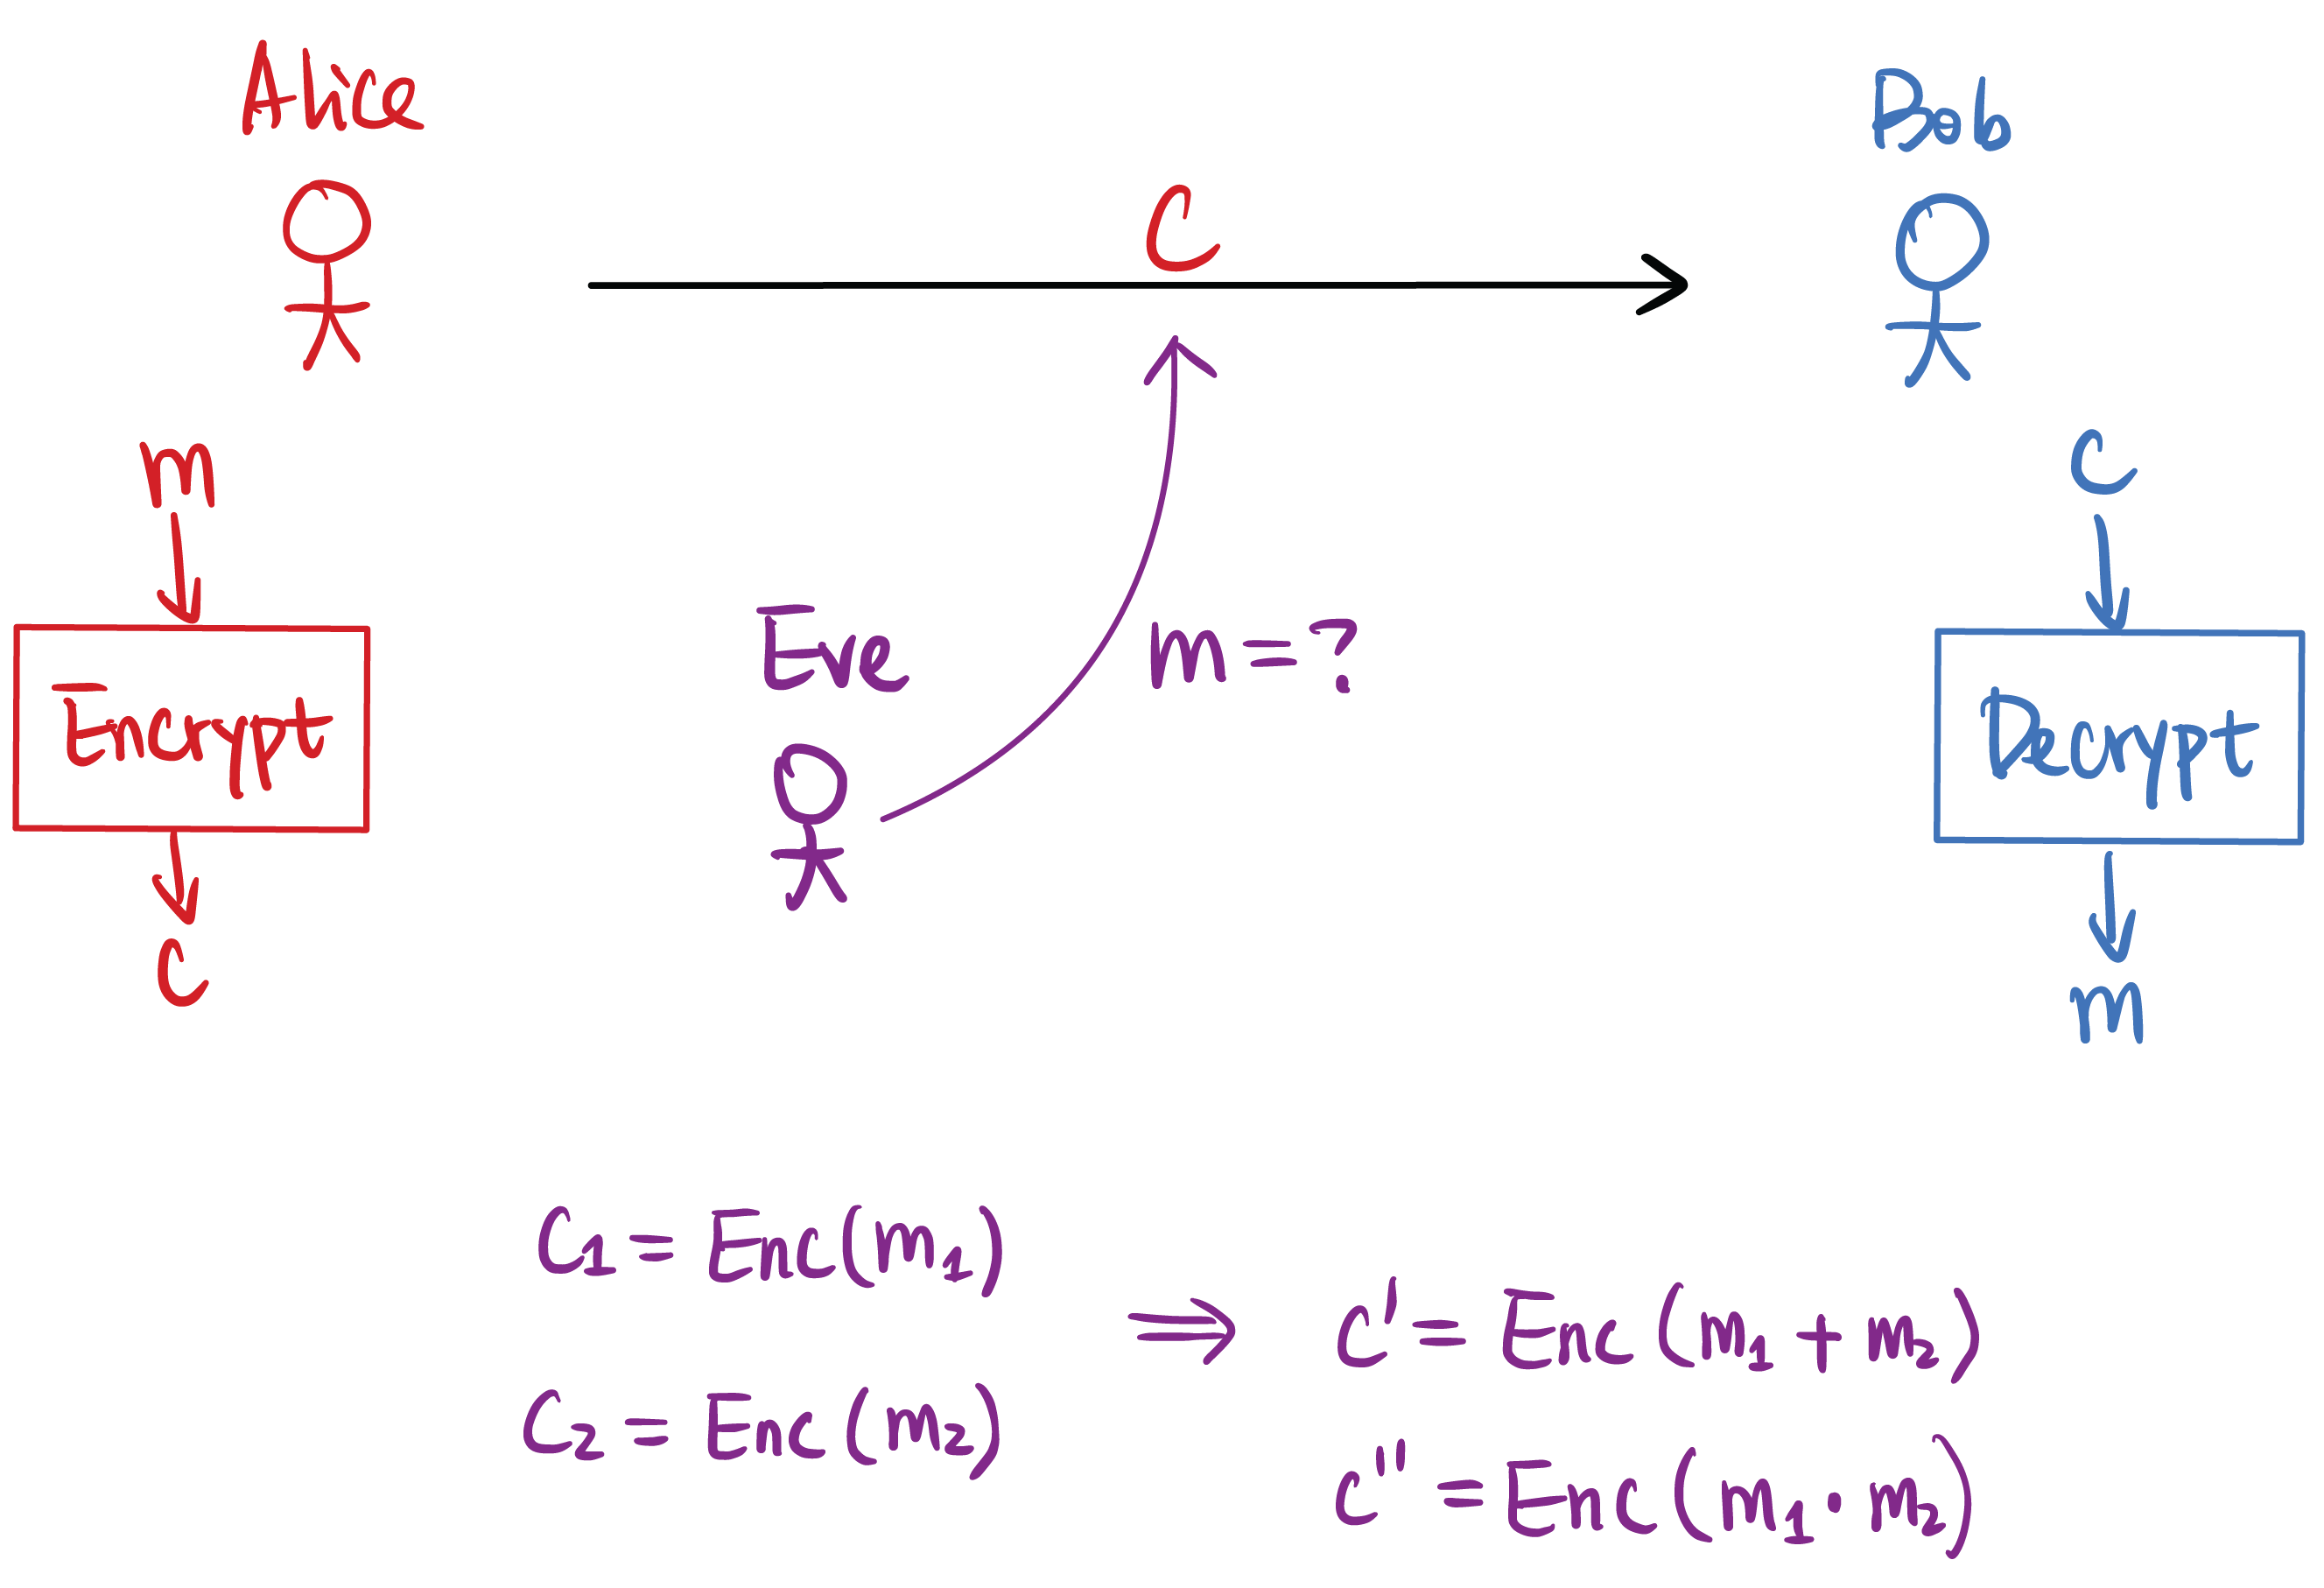
\includegraphics[width=0.9\textwidth]{images/2023-01-26/homomorphic_encryption.png}
\end{center}

We want to hopefully compute any function in polynomial time!

\begin{example*}[Outsourced Computation]
    Alice has some messages but doesn't have enough compute. There is a server that has \emph{a lot} of compute!

    \begin{center}
        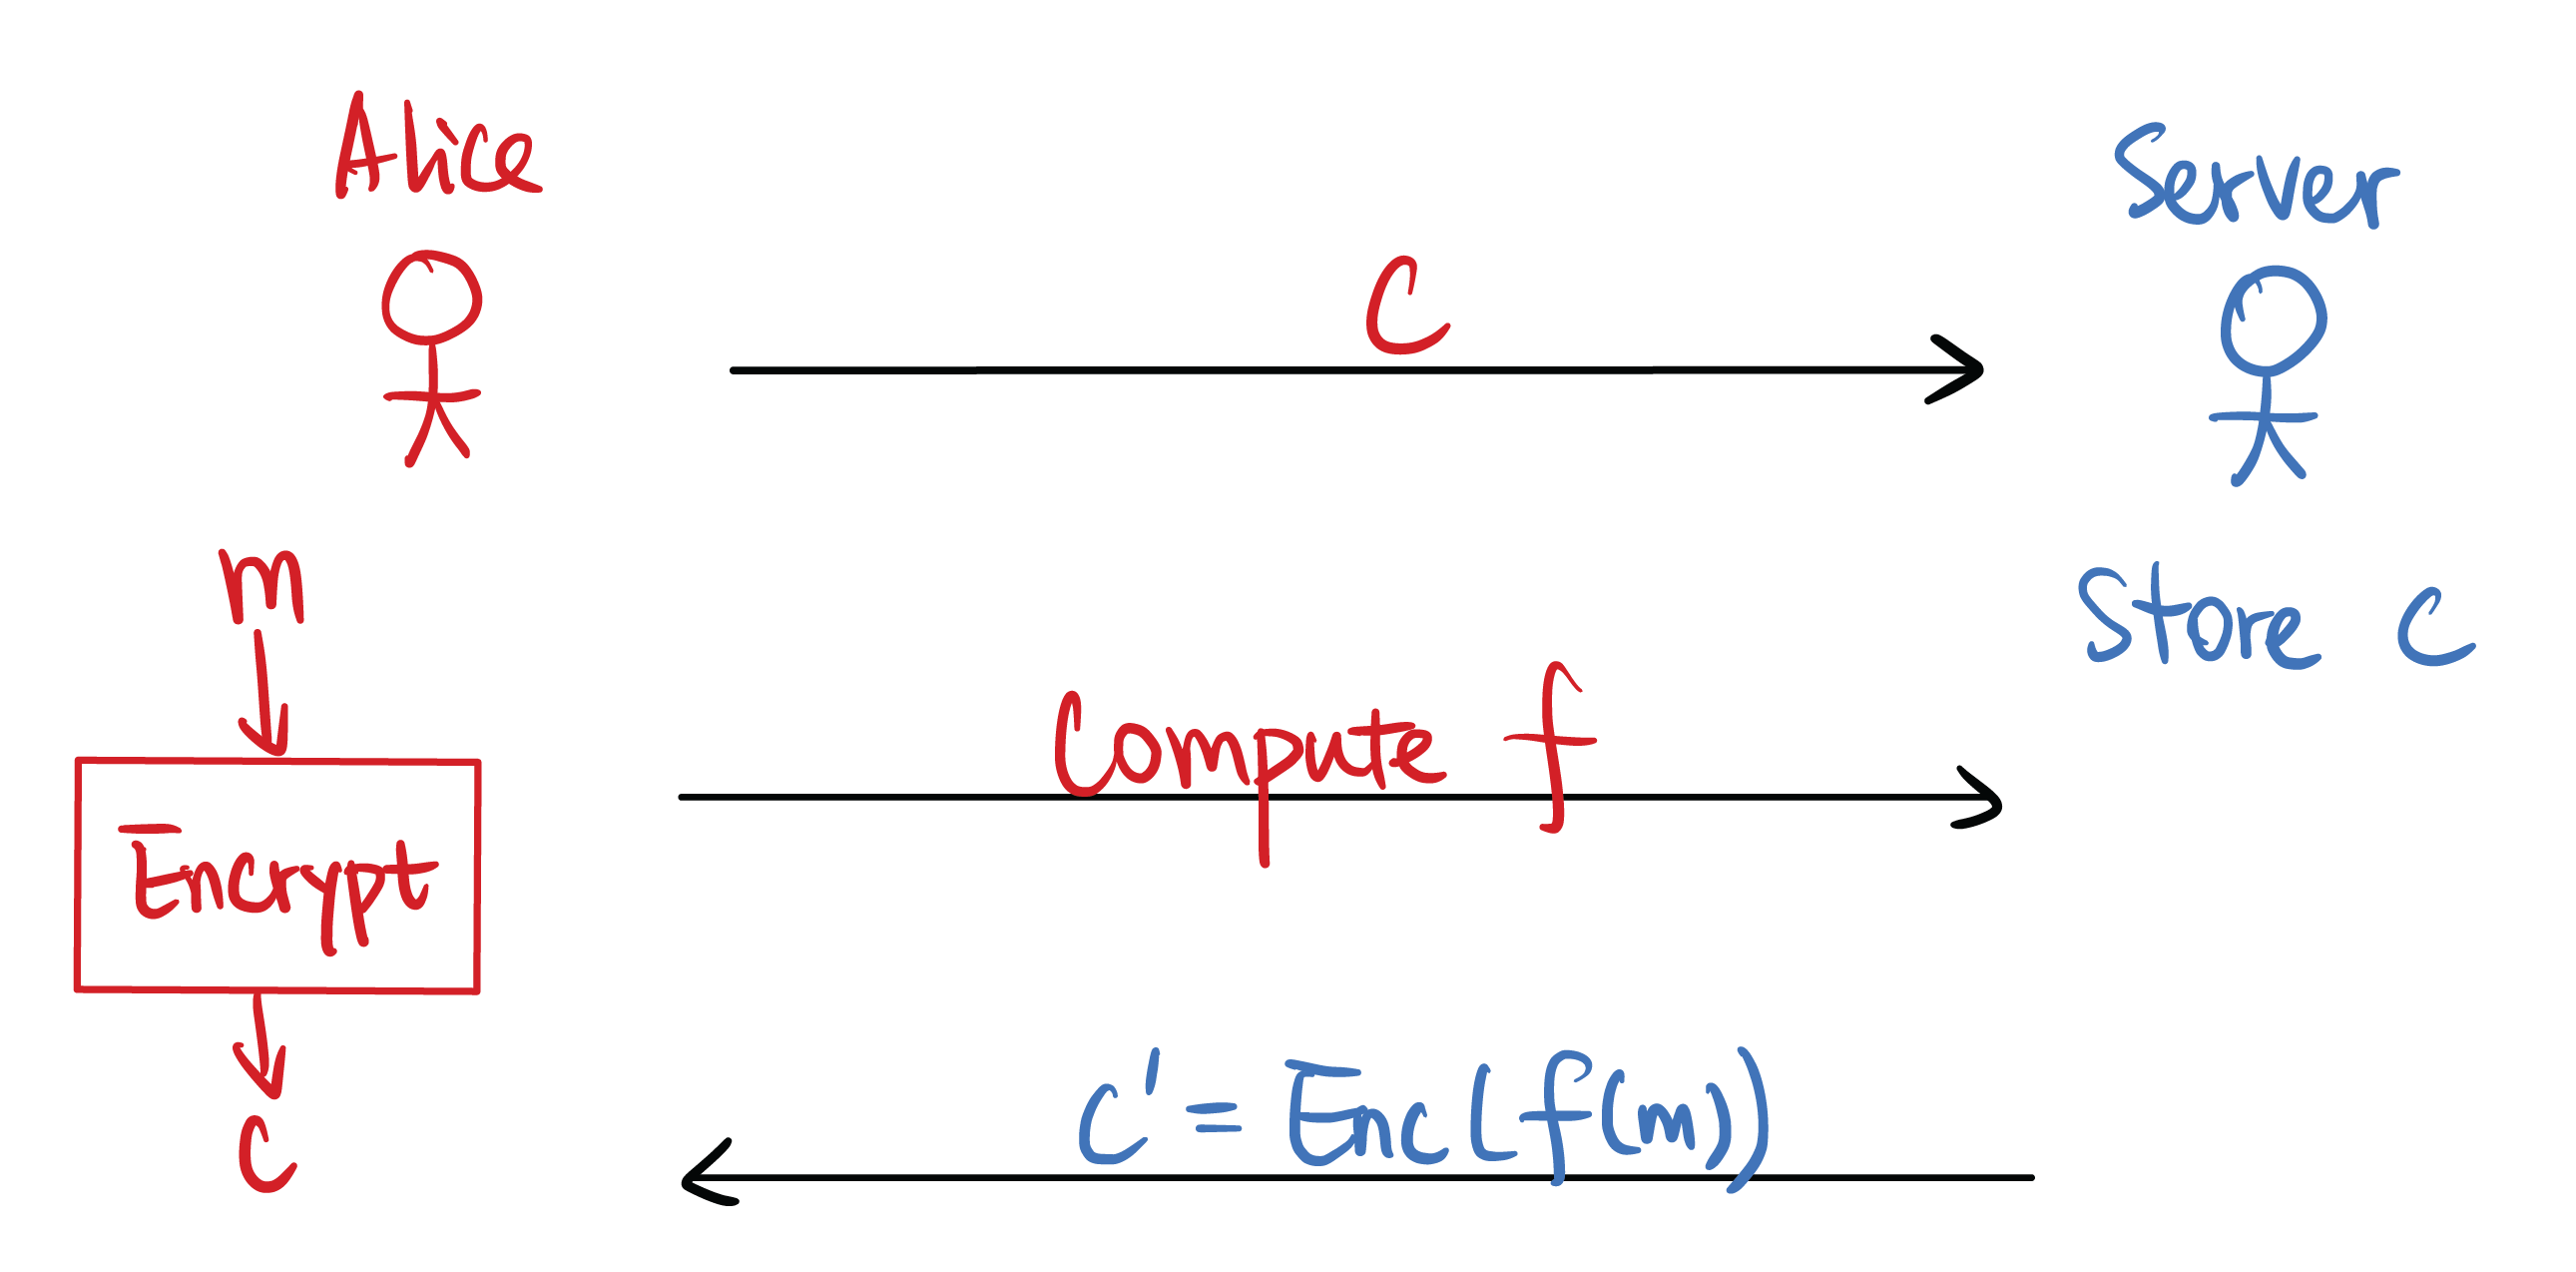
\includegraphics[width=0.9\textwidth]{images/2023-01-26/outsourced_computation.png}
    \end{center}

    Alice encrypts her data and stores it in the server. At some point, Alice might want to compute a function on the encrypted data on the server, without the server revealing the original data.

    This is an example of how fully homomorphic encryption can be useful.
\end{example*}

\begin{remark*}
    This problem was not solved until 2009 (when Peihan started her undergrad). Theoretically, it doesn't even seem that possible! Being able to compute functions on ciphertexts that correspond to functions on plaintexts.
\end{remark*}

To construct fully-homomorphic encryption, we'll be using lattice-based cryptography. This is also the only cryptographic primitive that is quantum-secure\footnote{Everything before this can be broken if quantum computers become mainstream!}.

\subsubsection{Further Topics}
We might cover some other topics:
\begin{itemize}
    \item Differential Privacy
    \item Crypto applications in machine learning
    \item Crypto techniques used in the blockchain\footnote{One important techniques is Zero-Knowledge proofs, for example.}
\end{itemize}
\emph{What else would you like to learn? What else do you want to understand?} Do go through the semester with these in mind! \emph{How do I log into Google? How do I send messages to friends?}

Peihan will collect responses at the start and middle of the semester to shape course content.

\subsection{A Quick Survey}
\emph{Peihan conducted the following poll in-class to gauge content for future lectures. \textbf{By all means, you don't need to know any/all of this going into this course! These will be self-contained in this course!}}

Do you know what the following means?
\begin{itemize}
    \item Polynomial-time algorithm.
    \item \textsf{NP}-hard problems.
    \item ``$a$ divides $b$'' ($a\mid b$)
    \item GCDs
    \item (Extended) Euclidean Algorithms
    \item Groups
    \item One-Time pads
    \item RSA encryption/signature
    \item Diffie-Hellman Key Exchange
    \item SHA (hash functions)
\end{itemize}

%!TEX root = ../notes.tex
\section{January 31, 2023}
\label{20230131}
\subsection{Logistics}
There's an EdStem post asking about topics you're interested, feel free to keep on posting!

We acknowledge the synchronization issues with Panopto. For now, if you want to watch the lecture recordings, you can use the Zoom link linked from the course home page. We can manually sync up EdStem but Panopto cannot be synced up, unfortunately.

\subsection{Encryption Schemes}
This lecture we'll cover encryption schemes. We briefly mentioned what encryption schemes were last class, we'll dive into the technical content: how we construct them, assumptions, RSA, ElGamal, etc.

Fundamentally, an encryption scheme protects message secrecy. If Alice wants to communicate to Bob, Alice will encrypt a message (plaintext) using some key which gives her a ciphertext. Sending the ciphertext through Bob using a public channel, Bob can use the key to decrypt the ciphertext and recover the message. An eavesdropper in the middle will have no idea what message has been transmitted.

\begin{center}
    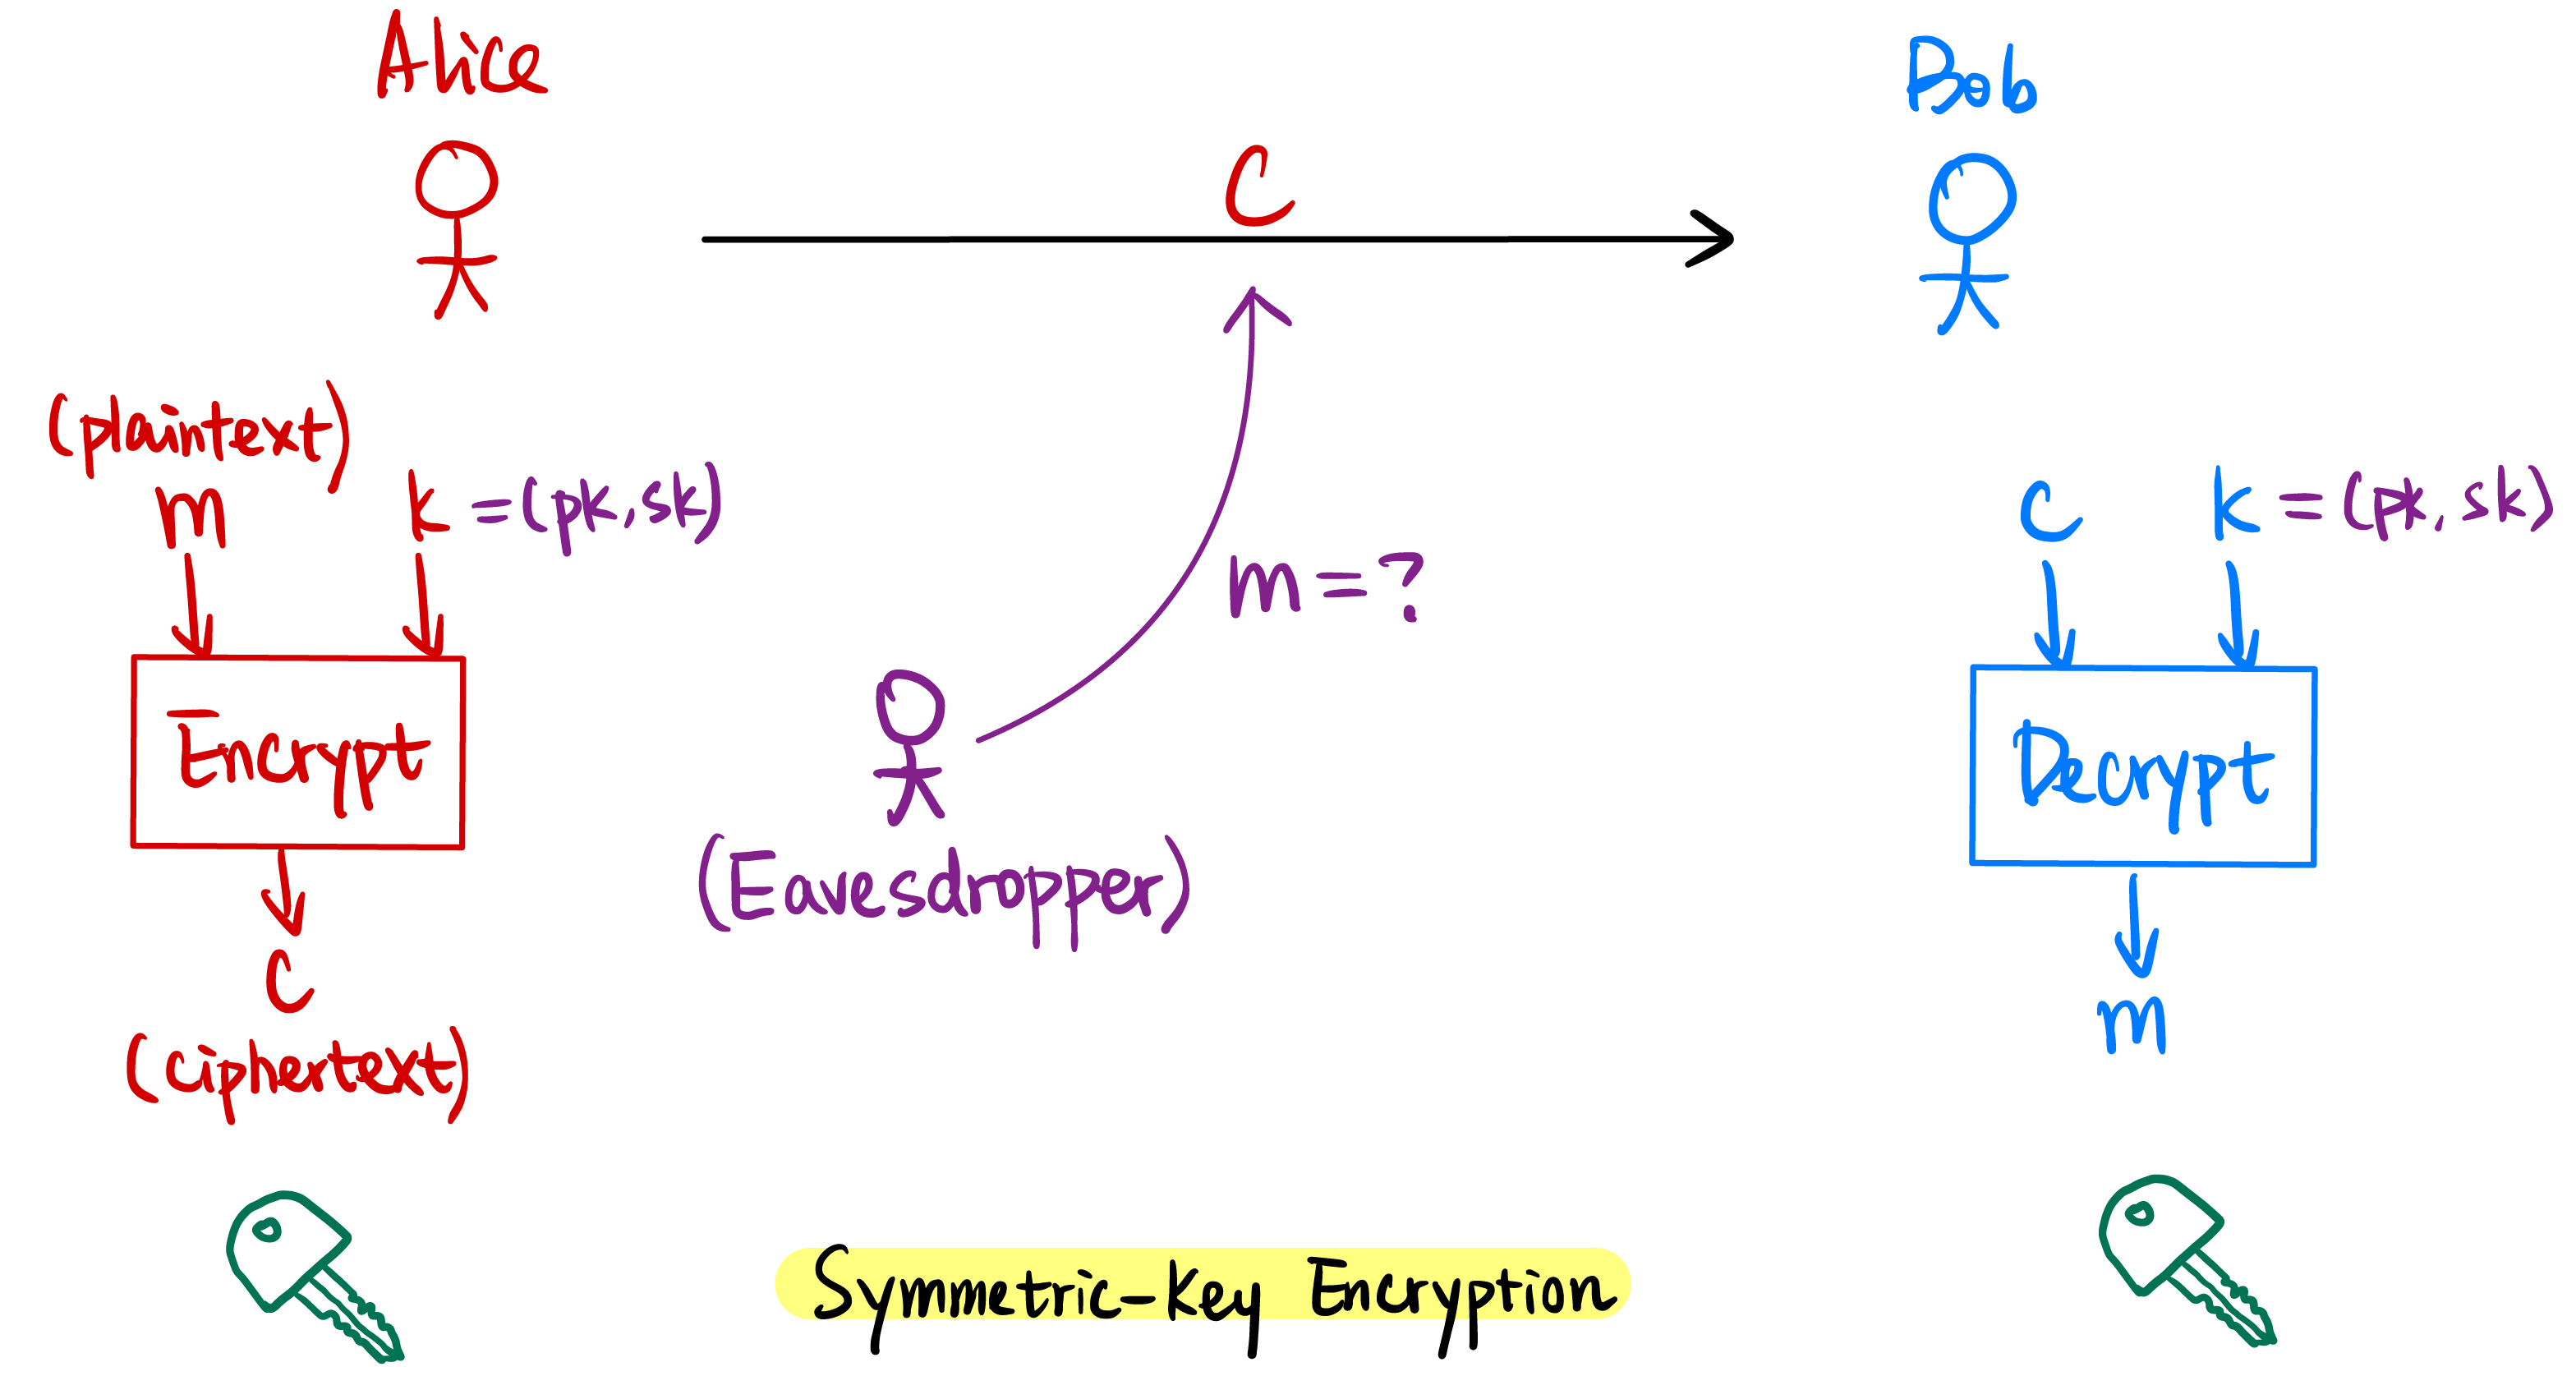
\includegraphics[width=0.8\textwidth]{images/2023-01-31/ske-intro.png}
\end{center}

In this case, they are using a shared key, which we called secret-key encryption or symmetric-key encryption.

A stronger version of private-key encryption is called public-key encryption. Alice and Bob do not need to agree on a shared secret key beforehand. There is a keypair $(pk, sk)$, a \emph{public} and \emph{private} key.

\begin{center}
    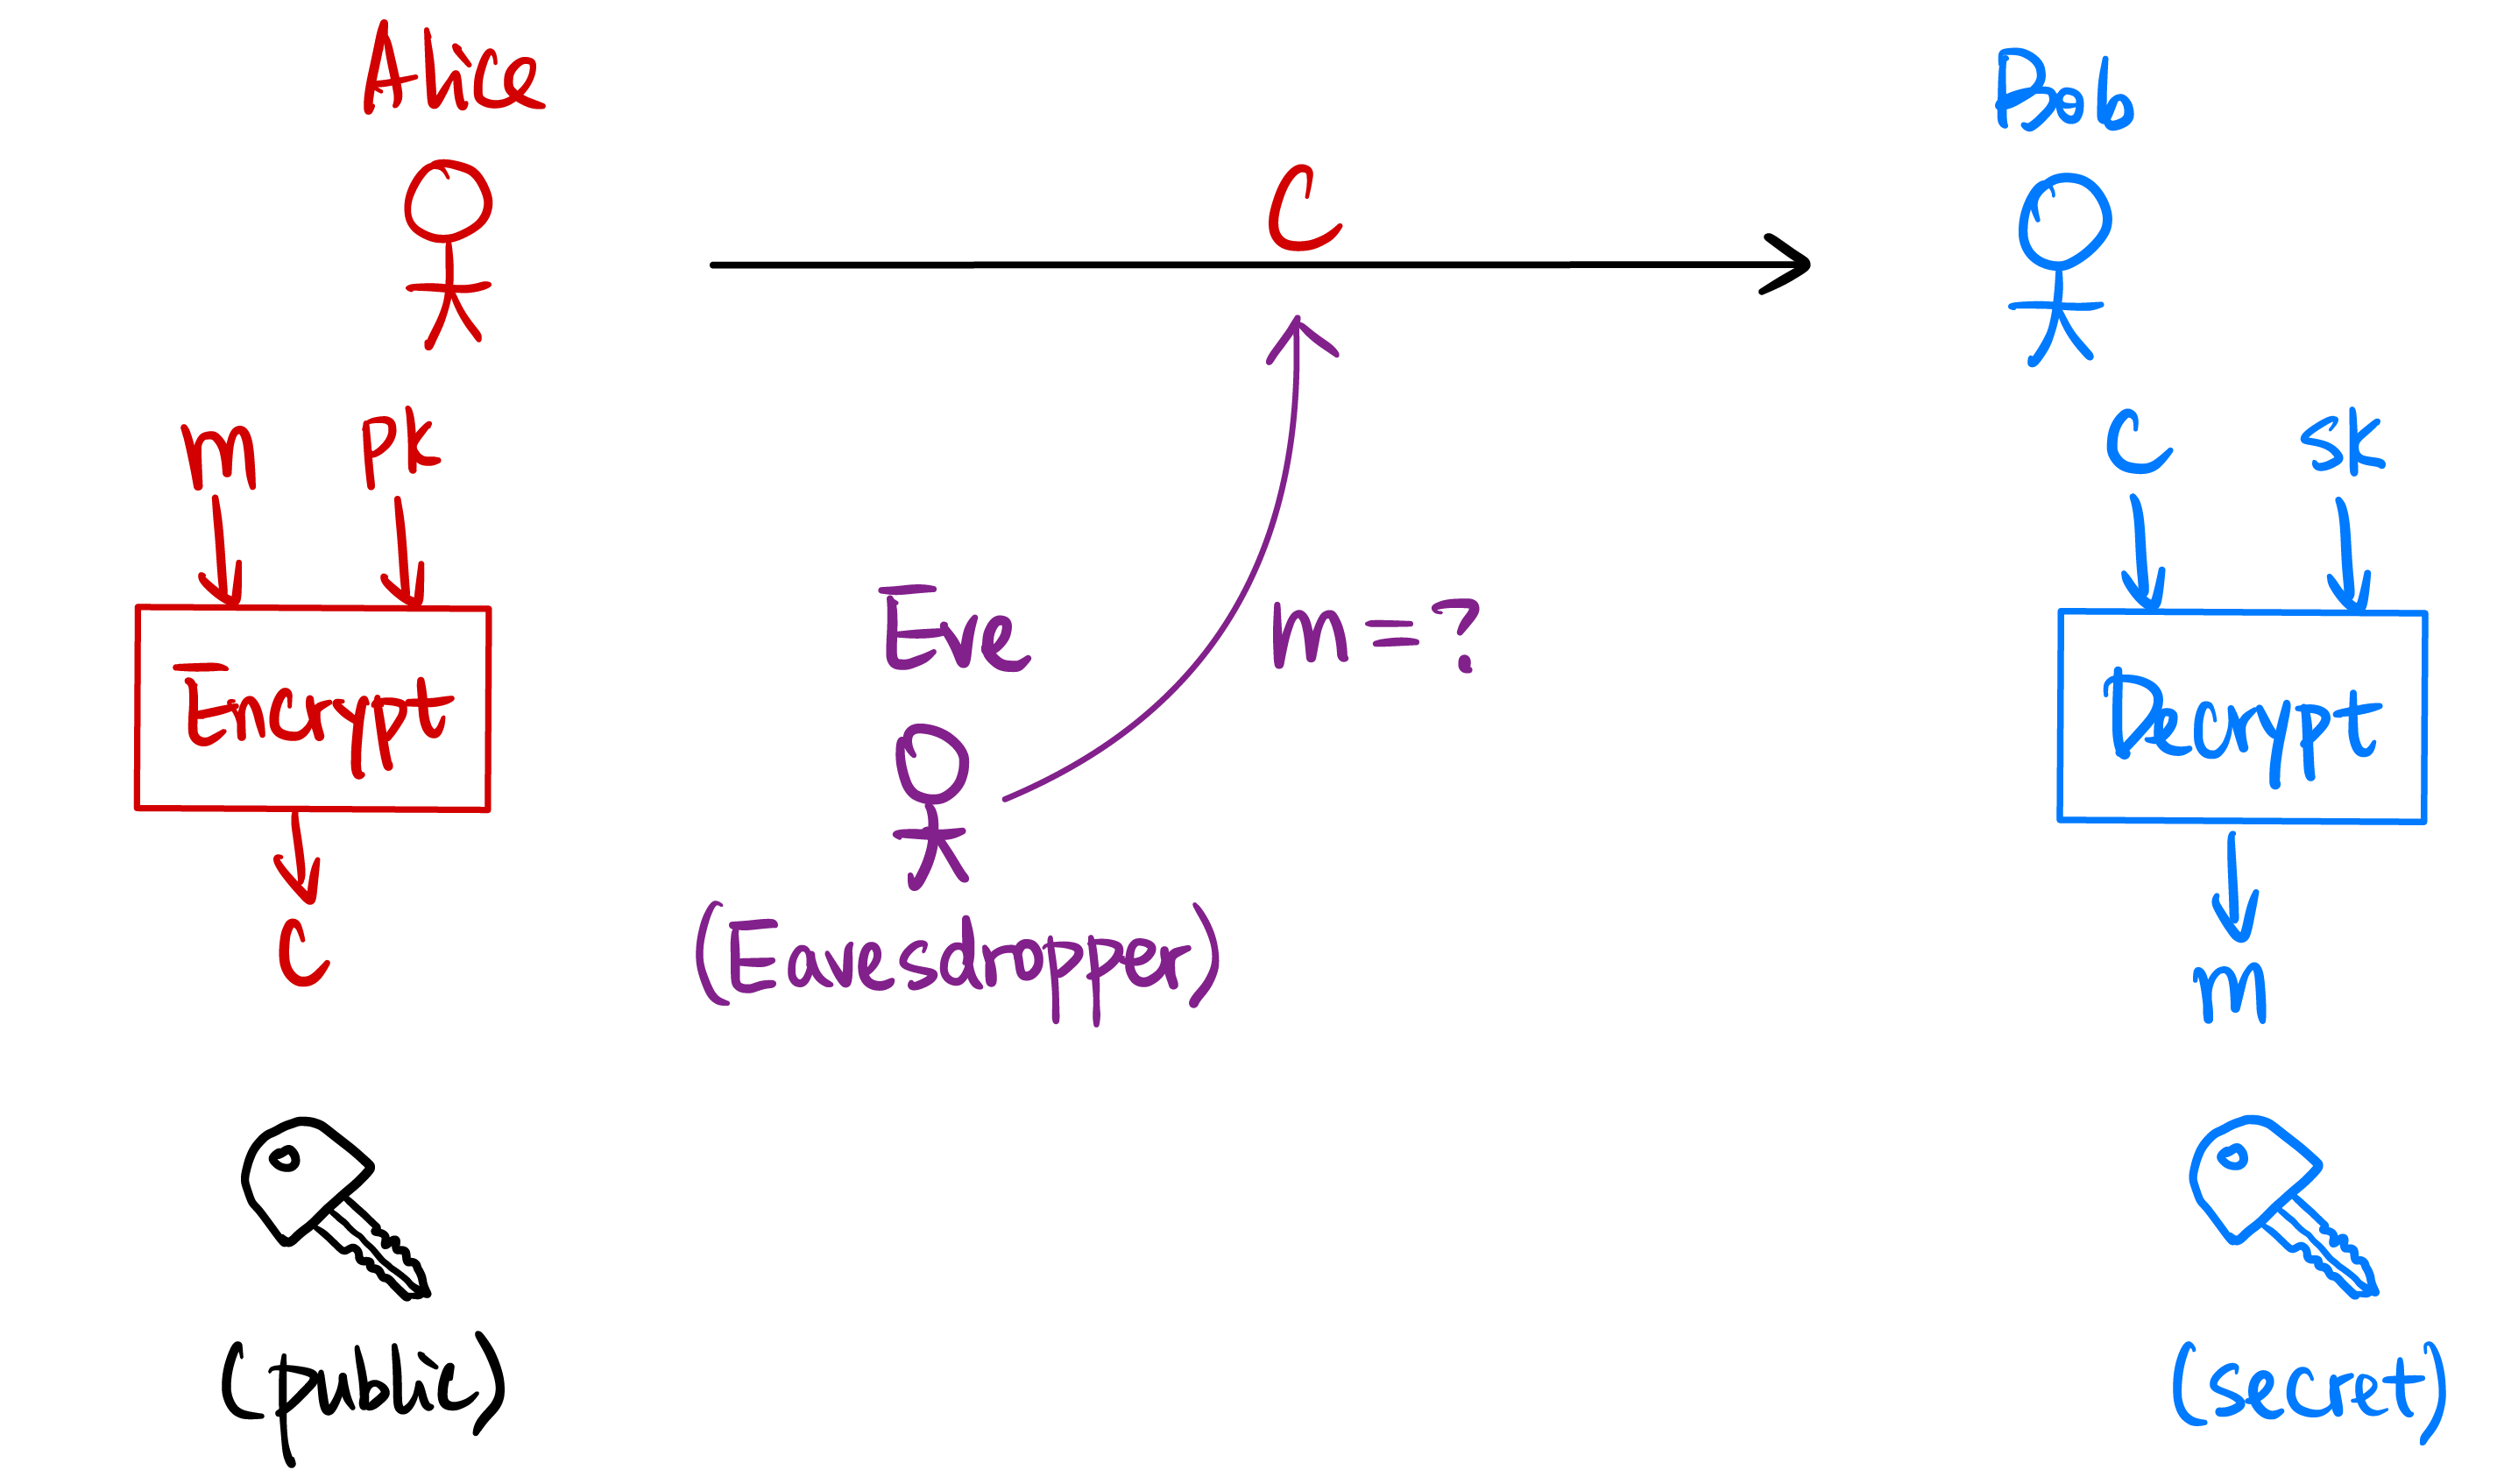
\includegraphics[width=0.8\textwidth]{images/2023-01-31/pke-intro.png}
\end{center}

\subsubsection{Syntax}
\begin{definition}[Symmetric-Key Encryption]
    A symmetric-key encryption (SKE) scheme contains 3 algorithms, $\Pi = (\mathsf{Gen}, \mathsf{Enc}, \mathsf{Dec})$.

    \begin{description}
        \item[Generation.] Generates key $k\leftarrow \mathsf{Gen}$.
        \item[Encryption.] Encrypts message $m$ with key $k$, $c\leftarrow \mathsf{Enc}(k, m)$, which we sometimes write as $\Enc_k(m)$.
        \item[Decryption.] Decrypts using key $k$ to retrieve message $m$, $m := \Dec(k, c)$, or written as $\Dec_k(c)$.
    \end{description}
    Note the notation $\leftarrow$ and $:=$ is different. In the case of generation and encryption, the produced key $k$ or $c$ follows a \emph{distribution} (is randomly sampled), but we had better want decryption to be deterministic in producing the message.
\end{definition}

\begin{definition}[Public-Key Encryption]
    A public-key encryption (PKE) scheme $\Pi = (\Gen, \Enc, \Dec)$ contains the same $3$ algorithms,

    \begin{description}
        \item[Generation.] Generate keys $(pk, sk)\leftarrow \Gen$.
        \item[Encryption.] Use the public key to encrypt, $c\leftarrow \mathsf{Enc}(pk, m)$ or $\Enc_{pk}(m)$.
        \item[Decryption.] Use the secret key to decrypt, $m:=\Dec(pk, c)$ or $\Dec_{pk}(c)$.
    \end{description}

\end{definition}

\begin{ques*}
    If we can construct public-key encryption, why do we even bother with secret-key encryption? We could just use the $(pk, sk)$ pair for our secret key, and this does the same thing.
\end{ques*}

\begin{enumerate}
    \item First of all, public-key encryption is almost always \emph{more expensive}. Symmetric-key encryption schemes give us efficiency.
    \item Public-key encryption relies on much stronger computational assumptions.
\end{enumerate}

\subsubsection{Symmetric-Key Encryption Schemes}
\begin{definition}[One-Time Pad]
    Secret key is a uniformly randomly sampled $n$ bit string $k\sampledfrom \{0, 1\}^n$.

    \begin{center}
        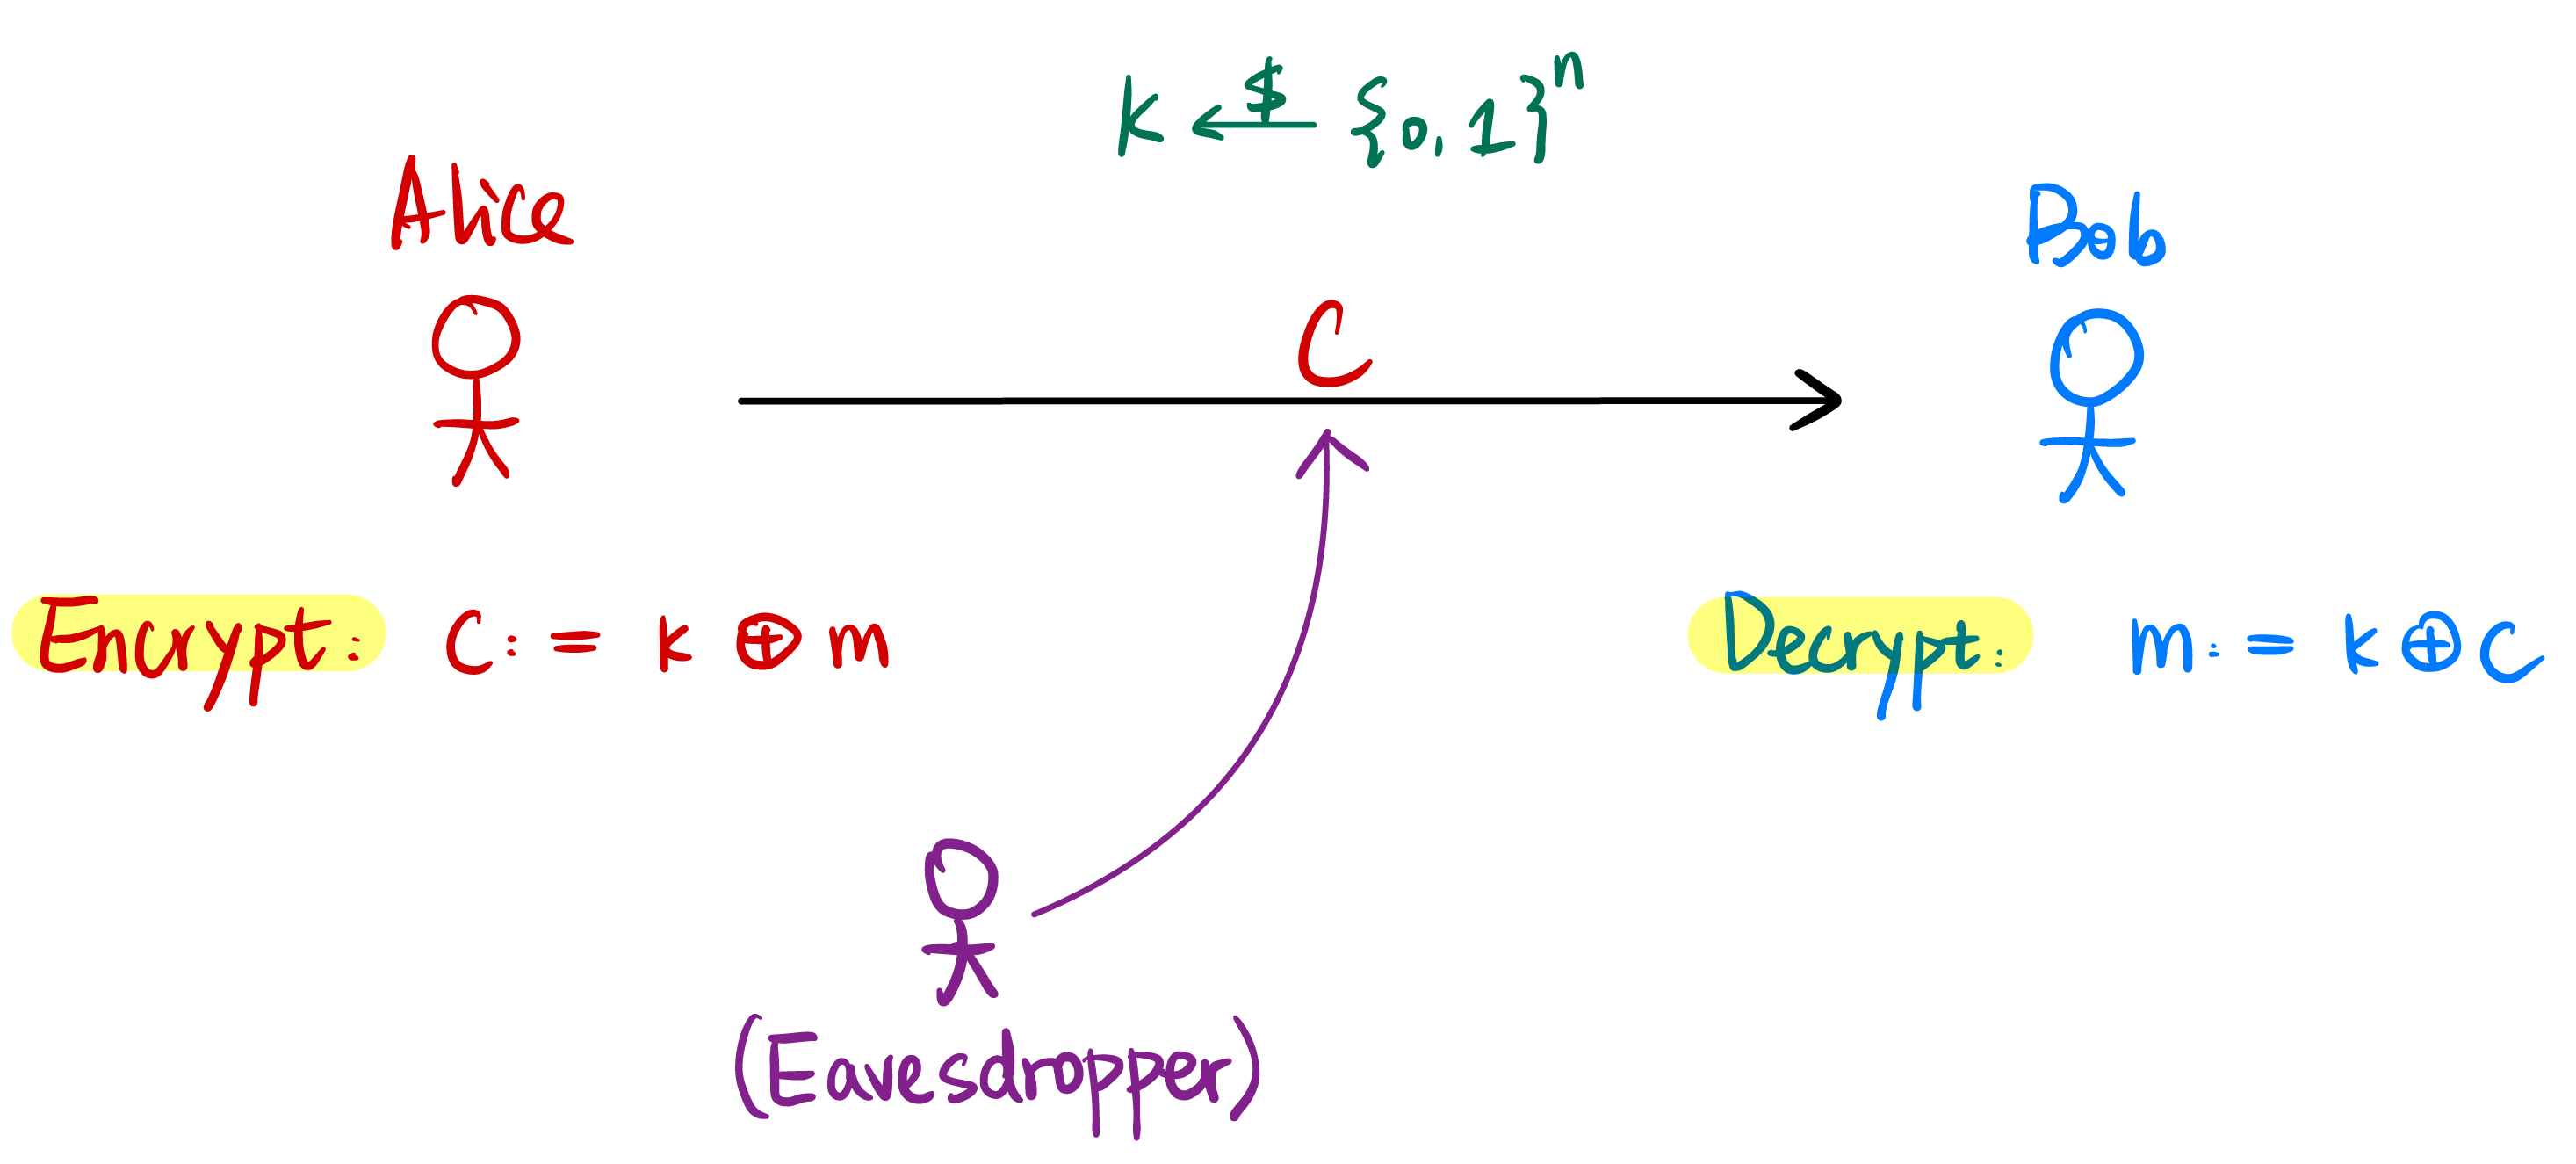
\includegraphics[width=0.7\textwidth]{images/2023-01-31/otp-defn.png}
    \end{center}

    \begin{description}
        \item[Encryption.] Alice uses the secret key and bitwise-$\mathsf{XOR}$ with the plaintext.
            \begin{align*}
                \begin{split}
                    \text{secret key}\quad k       & = 0100101 \\
                    \oplus\text{ plaintext}\quad m & = 1001001 \\ \eqline
                    \text{ciphertext}\quad c       & = 1101100
                \end{split}
            \end{align*}
        \item[Decryption.] Bob uses the secret key and again bitwise-$\mathsf{XOR}$ with the ciphertext
            \begin{align*}
                \begin{split}
                    \text{secret key}\quad k        & = 0100101 \\
                    \oplus\text{ ciphertext}\quad c & = 1101100 \\ \eqline
                    \text{plaintext}\quad c         & = 1001001
                \end{split}
            \end{align*}
    \end{description}

    This is widely used in cryptography, called \emph{masking} or \emph{unmasking}.
\end{definition}

\begin{ques*}
    Why is this correct?
\end{ques*}
An $\mathsf{XOR}$ done twice with the same choice bit $b$ is the identity. Or, an element is its own inverse with the $\mathsf{XOR}$ operator.

\begin{ques*}
    Why is this secure?
\end{ques*}

We can think about this as the distribution of $c$. $\forall m\in \{0, 1\}^n$, the encryption of $m$ is uniform over $\{0, 1\}^n$ (since $k$ was uniform).

Another way to think about this is that for any two messages $m_0, m_1\in\{0, 1\}^n$, $\Enc_k(m_0)\equiv \Enc_k(m_1)$. That is, the encryptions follow the \emph{exact same} distribution. In this case, they are both uniform, but this is not always the case.

\begin{ques*}
    Can we reuse $k$? Should we use the same key again to encrypt another message? Or, it is possible for the eavesdropper to extract information.
\end{ques*}

For example, $\Enc_k(m)$ is $c:= k\oplus m$, and $\Enc_k(m')$ is $c' := k\oplus m'$. If the two messages are the same, the ciphertexts are the same.

By $\mathsf{XOR}$ $c$ and $c'$, we get
\begin{align*}
    c\oplus c' & = (\cancel{k}\oplus m) \oplus (\cancel{k}\oplus m') \\
               & = m\oplus m'
\end{align*}
This is why this is an \emph{one-time} pad. This is a bit of an issue, to send an $n$-bit message, we need to agree on an $n$-bit message.

In fact, this is \emph{the best} that we can do.

\begin{theorem}
    \emph{Informally,} for perfect (information-theoretic\framedfootnote{That the distributions of ciphertexts are identical, that $\Enc_k(m_0)\equiv \Enc_k(m_1)$.}) security, the key space must be at least as large as the message space.
    \[|\mathcal{K}|\geq |\mathcal{M}|\]
    where $\mathcal{K}$ is the key space and $\mathcal{M}$ is the message space.
\end{theorem}

\begin{ques*}
    How can we circumvent this issue?
\end{ques*}

The high level idea is that we weaken our security guarantees \emph{a little}. Instead of saying that they have to be \emph{exactly the same} distribution, we say that they are \emph{hard to distinguish} for an adversary with limited computational power. This is how modern cryptography gets around these lower bounds in classical cryptography. We can make \emph{computational assumptions} about cryptography.

We can think about computational security,
\begin{definition}[Computational Security]\label{def:computational-security}
    We have \ul{computational security} when two ciphertexts have distribution that cannot be distinguished using a polynomial-time algorithm.
\end{definition}

\begin{definition}[Polynomial-Time Algorithm]
    A polynomial time algorithm $A(x)$ is one that takes input $x$ of length $n$, $A$'s running time is $O(n^c)$ for a constant $c$.
\end{definition}
\begin{definition}[\textsf{NP} Problem]
    A decision problem is in \ul{nondeterministic polynomial-time} when its solution can be \emph{verified} in polynomial time.
\end{definition}
\begin{example}[Graph 3-Coloring]
    Given a graph, does it have a $3$-coloring such that no two edges join the same color? For example,

    \begin{center}
        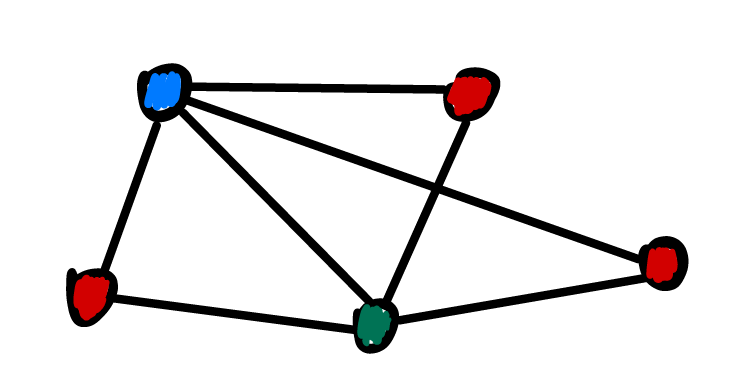
\includegraphics[width=0.4\textwidth]{images/2023-01-31/graph-coloring.png}
    \end{center}

    This can be \emph{verified} in polynomial time (we can check if such a coloring is a valid $3$-coloring), but it is computed in \textsf{NP} time.
\end{example}
\begin{definition}
    An \textsf{NP}-complete problem is a ``hardest'' problem in \textsf{NP}. Every problem in \textsf{NP} is at least as hard as an \textsf{NP}-complete problem.
\end{definition}

Right now, we assume $\mathsf{P}\neq\mathsf{NP}$. As of right now, there is no realistic algorithm that can solve any \textsf{NP} problem in polynomial-time.

Even further, we pick some problems not in $\mathsf{NP}$-complete, not in $\mathsf{P}$. We assume they are neither $\mathsf{NP}$-complete nor in $\mathsf{P}$ (we don't yet have a reduction, but we don't know if one could exist) The reasoning behind using these problems is as we have no good cryptoscheme relying solely on $\mathsf{NP}$-complete problems (we need something weaker).

\begin{center}
    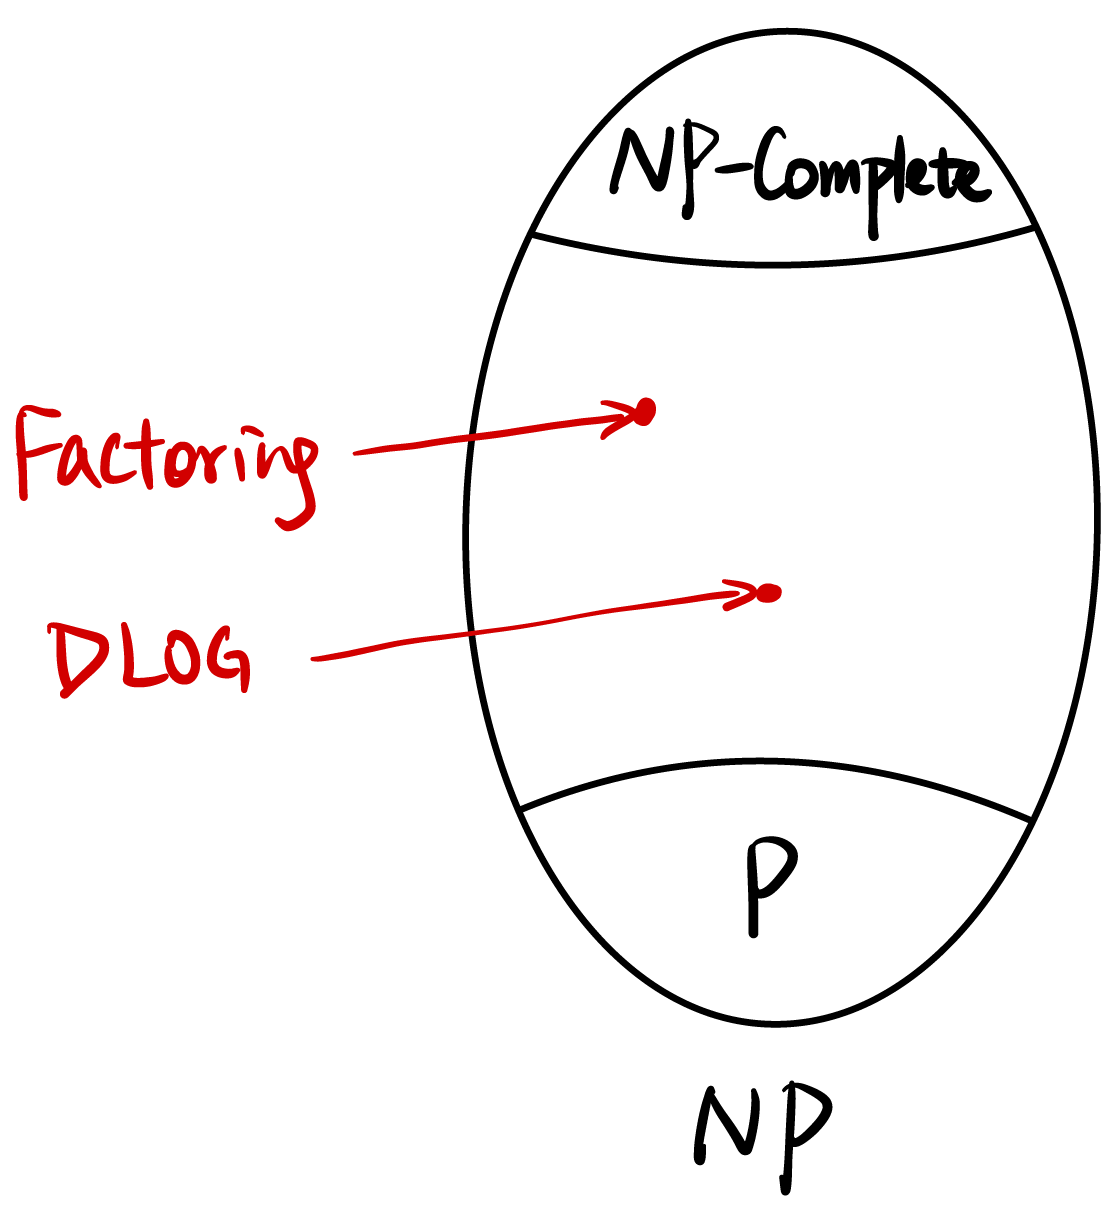
\includegraphics[width=0.4\textwidth]{images/2023-01-31/pnp-venn.png}
\end{center}

Going back to our definition of computational security \cref{def:computational-security},
\begin{definition*}[Computational Security]
    We say that the adversary is computationally bounded (is only a \emph{polynomial-time algorithm}), that $\forall \text{probabilic poly-time algorithm }\mathcal{A}$,
    \[\Enc_k(m_0)\overset{c}{\simeq}\Enc_k(m_1)\]
    Where $\overset{c}{\simeq}$ is ``computationally indistinguishable''.
\end{definition*}

What does it mean for distributions to be ``computationally indistinguishable''? Let's say Alice encrypts multiple messages $m_0, m_1, \dots$ to Bob and produces $c_0, c_1, \dots$. Even if Eve can see all plaintexts $m_i$ in the open and ciphertexts $c_i$ in the open, between known $m_0, m_1$ and randomly encrypting one of them $c\leftarrow \Enc_{k}(m_b)$ where $b\sampledfrom \{0, 1\}$, the adversary cannot determine what the random choice bit $b$ is. That is, $\Pr[b = b'] \leq \frac{1}{2} + \mathsf{negligible}(\lambda)$\footnote{$\lambda$ is the security parameter, roughly a measure of how secure the protocol is. If it were exactly equal $\frac{1}{2}$, we have information-theoretic security.}. This is Chosen-Plaintext Attack (CPA) Security.

\begin{center}
    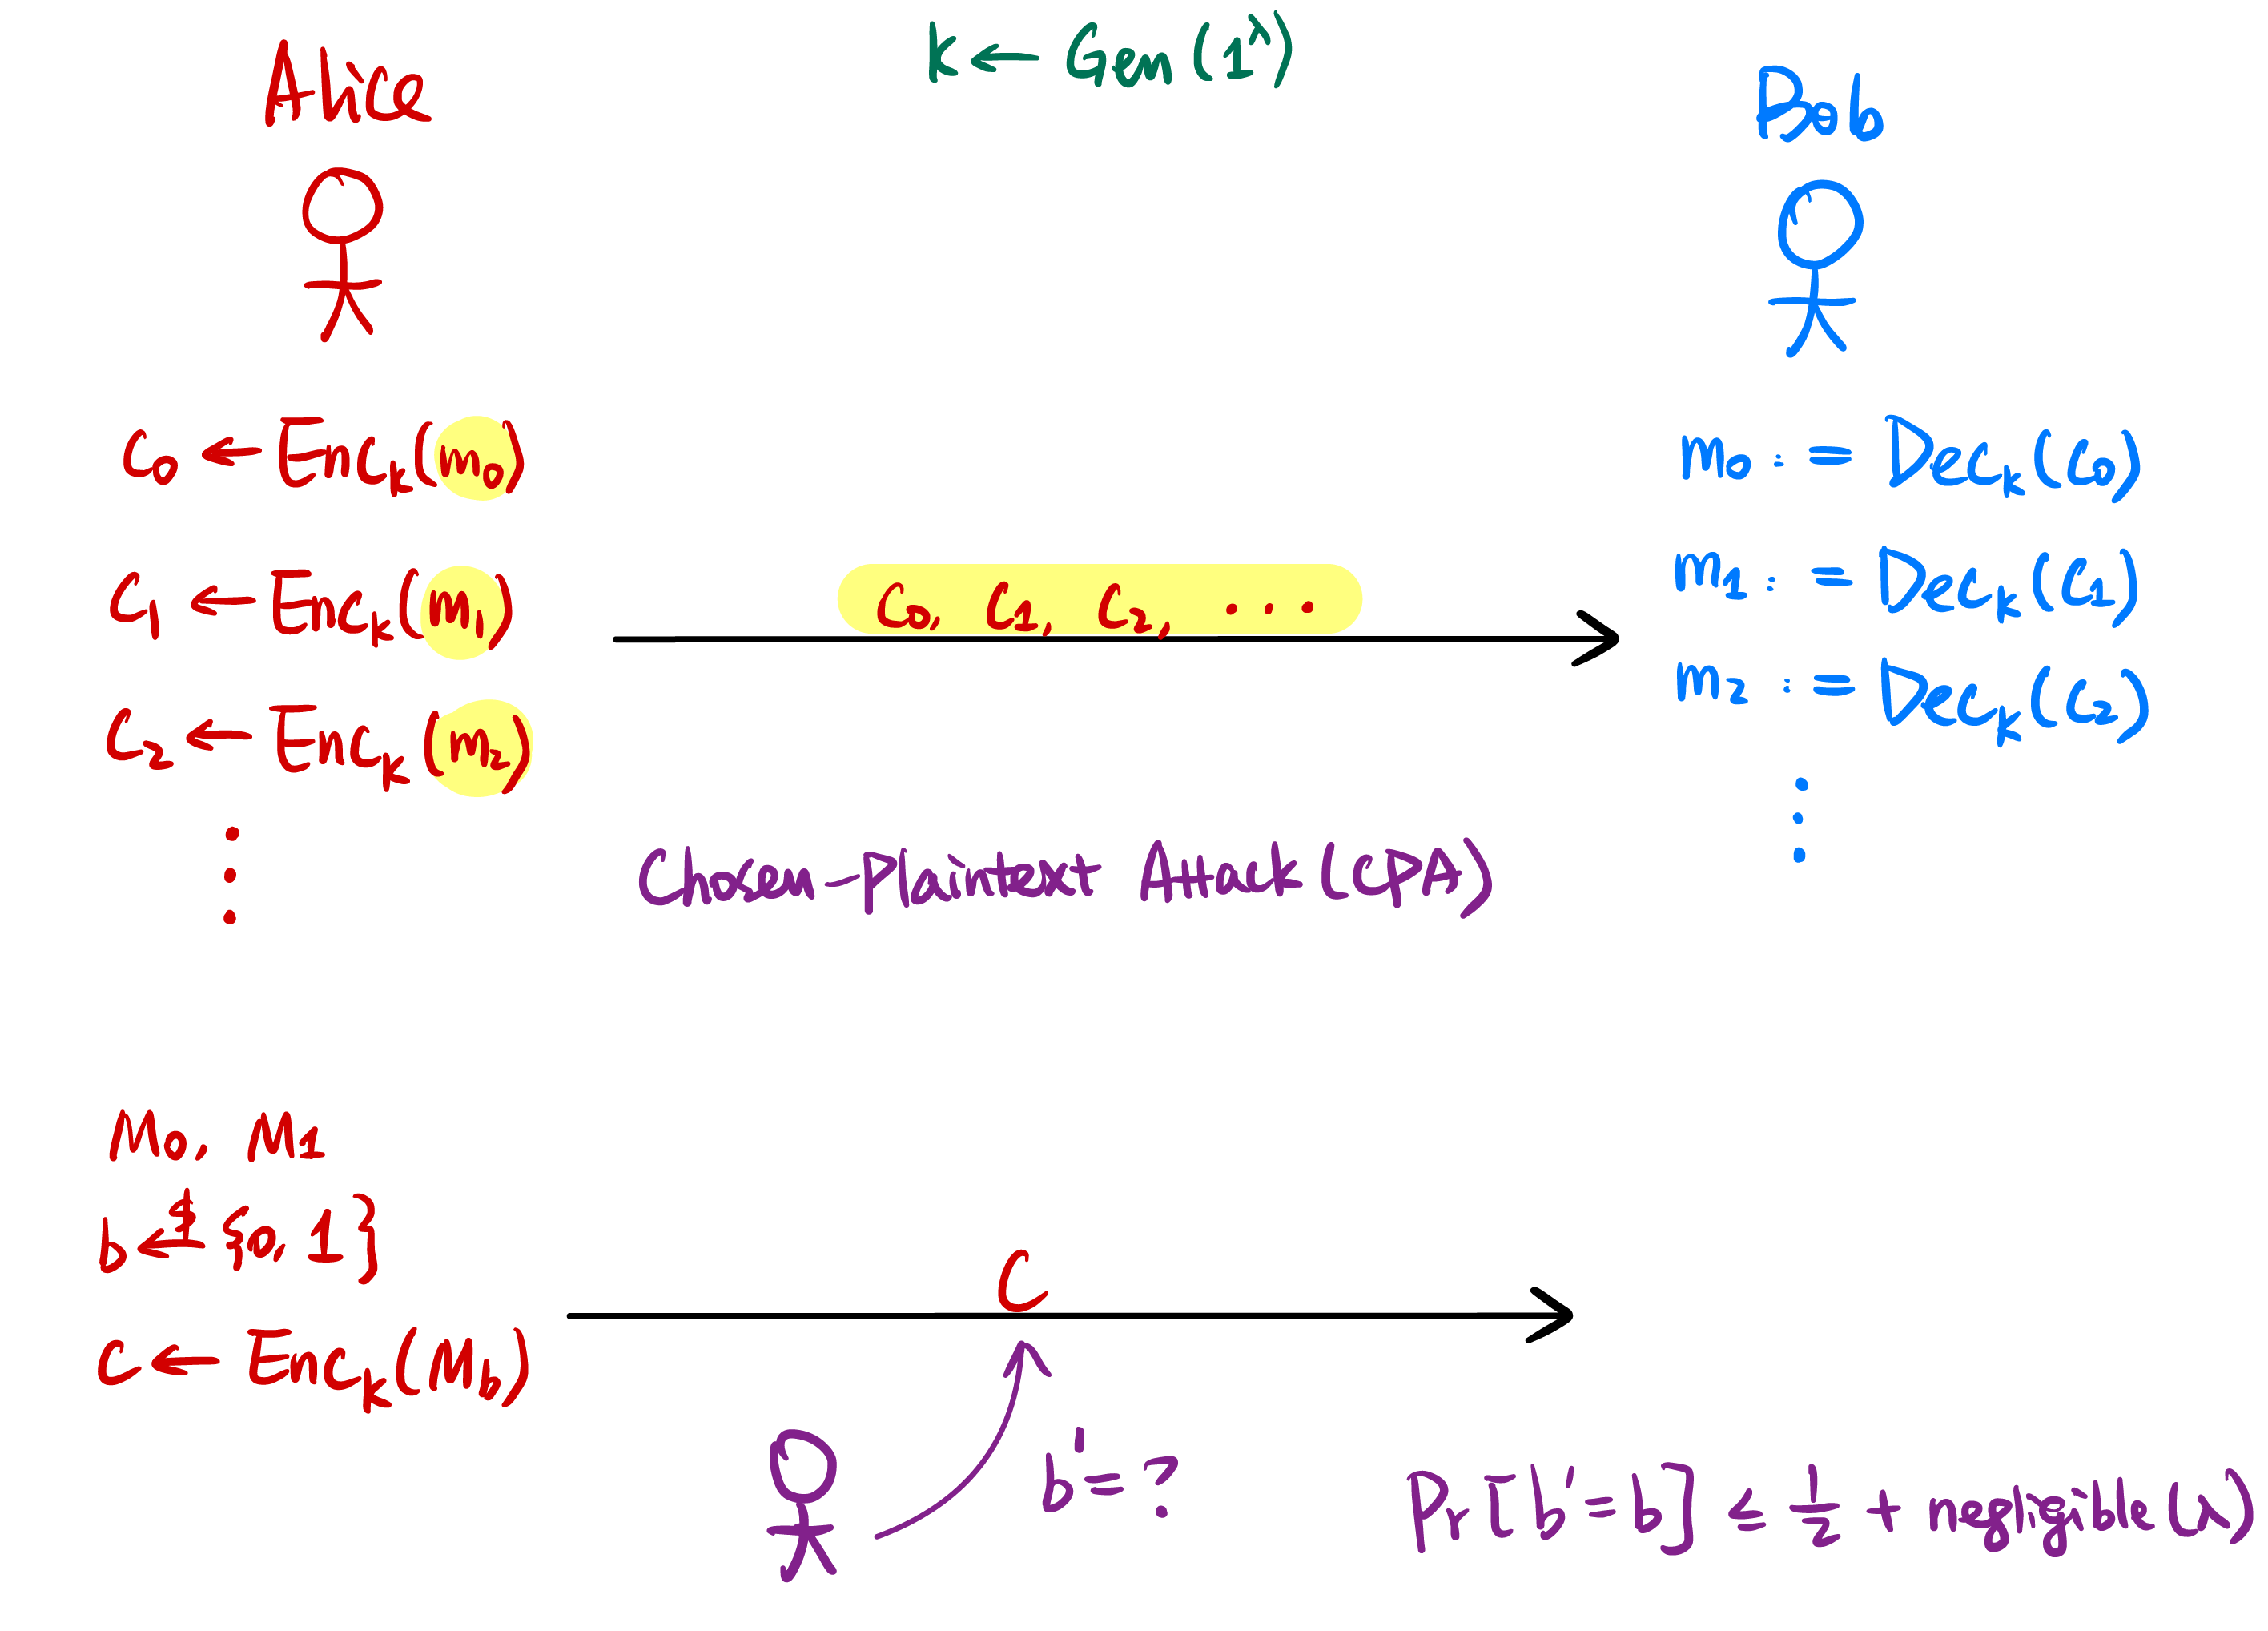
\includegraphics[width=0.8\textwidth]{images/2023-01-31/computational-security.png}
\end{center}

For a key generated $k\leftarrow \Gen(1^\lambda)$.

Theoretically, for $\lambda$ a security parameter and an adversary running in time $\mathsf{poly}(\lambda)$, the adversary should have distinguishing advantage $\negligible(\lambda)$ where
\[\negligible(\lambda) \ll \frac{1}{\lambda^c}\qquad \forall\text{ constant }c.\]

In practice, we set $\lambda = 128$. This means that the best algorithm to break the scheme (e.g. find the secret key) takes time $\sim 2^\lambda$. Currently, this is longer than the age of the universe.

\begin{example}
    \textbf{If the best algorithm is a brute-force search for $k$, what should our key length be?}

    It can just be a $\lambda$ bit string.
\end{example}
\begin{example*}
    \textbf{What if the best algorithm is no longer a brute-force search, but instead for a key length $l$ takes $\sim \sqrt{2^l}$?}

    Our key length should be $2\lambda$. Doing the math, we want $\sqrt{2^l} \equiv 2^\lambda$, solving for $l$ gives $2\lambda$.
\end{example*}

Going back to the original problem of secret-key encryption, how can we use our newfound cryptographic constructions to improve this?

From a pseudorandom function/permutation (PRF/PRP), we can reuse our secret key by passing it through the pseudorandom function.

The current practical construction for PRD/PRP is called the block cipher, and the standardized implementation is AES\footnote{Determined via a competition for such an algorithm in the early 2000s. }

It is a computational assumption\footnote{Based on heuristic, not involving any number theory!} that the AES construction is secure, and the best attack is currently a brute-force search (in both classical and quantum computing realms).

\subsubsection{Public-Key Encryption Schemes}
Using computational assumptions, we explore some public-key encryption schemes.

\begin{description}
    \item[RSA Encryption.] This is based on factoring/RSA assumption, that factoring large numbers is hard.
    \item[ElGamal Encryption.] This is based on the discrete logarithm/Diffie-Hellman Assumption, that finding discrete logs in $\ZZ_p$ is hard.
    \item[Lattice-Based Encryption.] The previous two schemes are not quantum secure. Quantum computation will break these schemes. Lattice-based encryption schemes are post-quantum secure. They are associated with the difficulty of finding `short' vectors in lattices\footnote{Covered later in class, we focus on the first two now.}.
\end{description}

Another thing worth mentioning is that
\begin{theorem}
    \emph{(Very informally,)} It is impossible to construct PKE from SKE in a black-box way. This is called ``black-box separation''.
\end{theorem}

We first need to define a bit of number-theory background.
\begin{definition}
    We denote $a\mid b$ as $a$ \ul{divides} $b$, that is, there is integer $c$ such that $b = a\cdot c$.
\end{definition}
\begin{definition}
    The $\gcd(a, b)$ is the greatest common divisor of $a, b$. If $\gcd(a, b) = 1$, then $a, b$ are coprime.
\end{definition}
\begin{ques*}
    How do we compute $\gcd$? What is its time complexity?
\end{ques*}
\begin{example*}
    We use the Euclidean Algorithm. Take $\gcd(12, 17)$,
    \begin{align*}
        17\mod{12} & = 5 \\
        12 \mod{5} & = 2 \\
        5\mod{2}   & = 1 \\
        2\mod{1}   & = 0
    \end{align*}
    or take $\gcd(12, 18)$
    \begin{align*}
        18\mod{12} & = 6 \\
        12\mod{6}  & = 0
    \end{align*}
\end{example*}
If we have two bitstrings of length $n$ bits, what is the running time of the Euclidan Algorithm?

\begin{center}
    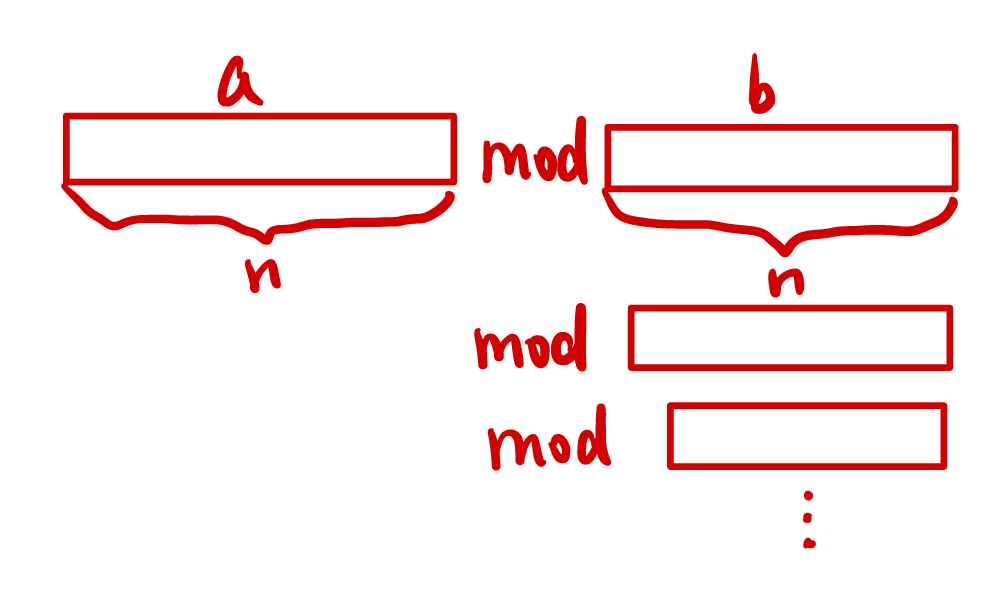
\includegraphics[width=0.3\textwidth]{images/2023-01-31/euclidean-algo.png}
\end{center}

Very informally, we see that every step, the length of $a, b$ decrease by approximately $1$ bit. Then, finding $\gcd$ is roughly order $O(n)$.

\begin{definition}[Mod]
    $a\mod{N}$ is the remainder of $a$ when divided by $N$.

    $a\equiv b\pmod{N}$ means when $a$ and $b$ are \ul{congruent modulo} $N$. That is, $a\mod N = b\mod N$.
\end{definition}

\begin{ques*}
    How might we compute $a^b\mod N$? What is the time complexity? Let $a, b, N$ be $n$-bit strings.
\end{ques*}

Na\"ively, we can repeatedly multiply. But this takes $b$ steps ($2^n$).

We can `repeatedly square'. For example, we can get to $a^8$ faster by getting $a^2$, squaring to get $a^4$, and again to get $a^8$. We can take the bitstring of $b$ and determine how to compute this.

\begin{example*}
    If $b = 100101_2$, we take $a\cdot a^4\cdot a^{32}\mod N$ which can be calculated recursively (an example is given in the first assignment).
\end{example*}

The time complexity of this is order $O(n)$ for $n$-bit $a, b, N$\footnote{Not exactly order $n$, we should add the complexity of multiplication. However, this should be bounded by $N$ since we can log at every step.}.

\begin{theorem}[Bezout's Theorem, \emph{roughly}]
    If $\gcd(a,N) = 1$, then $\exists b$ such that
    \[a\cdot b \equiv 1\pmod{N}.\]
    This is to say, $a$ is \ul{invertible modulo} $N$. $b$ is its inverse, denoted as $a^{-1}$.
\end{theorem}
\begin{ques*}
    How do we compute $b$?
\end{ques*}
We can use the Extended Euclidean Algorithm!
\begin{example*}
    We write linear equations of $a$ and $N$ that sum to $1$, using our previous Euclidean Algorithm. Take the previous example $\gcd(12, 17)$,
    \begin{align*}
        17\mod{12} & = 5 \\
        12 \mod{5} & = 2 \\
        5\mod{2}   & = 1 \\
        2\mod{1}   & = 0
    \end{align*}
    We write this as
    \begin{align*}
        5 & = 17 - 12\cdot 1                         \\
        2 & = 12 - 5\cdot 2 = 12\cdot x + 17\cdot y  \\
        1 & = 5 - 2\cdot 2 = 12\cdot x' + 17\cdot y'
    \end{align*}
    where we substitute the linear combination of $5$ into $5$ on line $2$, substitute linear combination of $2$ into $2$ on line $1$, each producing another linear combination of $12, 17$.

    If $\gcd(a, N) = 1$, we use the Extended Euclidean Algorithm to write $1 = a\cdot x + N\cdot y$, then $1\equiv a\cdot x\pmod{N}$.
\end{example*}

\begin{definition}[Group of Units mod $N$]
    We have set
    \[\ZZ_N^\times:= \left\{ a\mid a\in [1, N-1], \gcd(a, N) = 1 \right\}\]
    which is the group of units modulo $N$ (they are units since they all have an inverse by above).
\end{definition}
\begin{definition}[Euler's Phi Function]
    Euler's phi (or totient) function, $\phi(N)$, counts the number of elements in this set. That is, $\phi(N) =  |\ZZ_N^\times|$.
\end{definition}
\begin{theorem}[Euler's Theorem]
    For all $a, N$ where $\gcd(a, N) = 1$, we have that \[a^{\phi(N)} \equiv 1\pmod{N}.\]
\end{theorem}

With this, we can start talking about RSA.

\subsubsection{RSA}
We first define the RSA assumption.
\begin{definition}[Factoring Assumption]
    Given two $n$-bit primes $p, q$, we compute $N = p\cdot q$. Given $N$, it's computationally hard to find $p$ and $q$ (classically).
\end{definition}
\begin{definition}[RSA Assumption]
    Given two $n$-bit primes, we again compute $N = p\cdot q$, where $\phi(N) = (p-1)(q-1)$. We choose an $e$ such that $\gcd(e, \phi(N)) = 1$ and compute $d \equiv e^{-1}\pmod{\phi(N)}$.

    Given $N$ and a random $y\sampledfrom \ZZ_{N}^\times$, it's computationally hard to find $x$ such that $x^e\equiv y\pmod{N}$.

    \begin{center}
        
\includegraphics[width=0.4\textwidth]{images/2023-01-31/rsa.png}
    \end{center}

    However, given $p, q$, it's easy to find $d$. We know $\phi(N) = (p-1)(q-1)$, so we can compute $d$ from $e$ by running the Extended Euclidean Algorithm. Then, taking $(x^e)^d\equiv x^{ed}\equiv x$ which allows us to extract $x$ again.
\end{definition}

Encrypting is exactly raising by power $d$, and decrypting is raising again by power $e$.

Remaining questions:
\begin{itemize}
    \item How can we generate primes $p, q$?
    \item How can we pick $e$ such that $\gcd(e, \phi(N)) = 1$?
    \item What security issues can you see?
\end{itemize}

We'll continue next class.
%!TEX root = ../notes.tex
\section{February 2, 2023}
\label{20230202}
\subsection{RSA Encryption, \emph{continued}}
\recall that the RSA encryption algorithm contains 3 components:
\begin{description}
    \item[$\Gen(1^\lambda)$:] Generate two $n$-bit primes $p, q$. We compute $N = p\cdot q$ and $\phi(N) = (p-1)(q-1)$. Choose $e$ such that $gcd(e, \phi(N)) = 1$. We compute $d = e^{-1}\mod{\phi(N)}$. Our public key $pk = (N, e)$, our secret key is $sk = d$.
    \item[$\Enc_{pk}(m)$:] $c = m^e\mod{N}$.
    \item[$\Dec_{sk}(c)$:] $m = c^d\mod{N}$.
\end{description}
We have a few remaining questions:
\begin{enumerate}
    \item How do we generate 2 primes $p, q$?
    \item How do we choose such an $e$?
    \item How do we compute $d = e^{-1}\mod{\phi(N)}$?
    \item How do we efficiently compute $m^e\mod{N}$ and $c^d\mod N$.
\end{enumerate}
How do we resolve these issues to ensure the $\Gen$ step is efficient (polynomial time).
\begin{enumerate}
    \item We pick an arbitrary number $p$ and check for primality efficiently (using Miller Rabin, a probabilistic primality test). We pick random numbers until they are prime. Since primes are `pretty dense' in the integers, this can be done efficiently.
    \item We can also guess! Since we're unsure whether coprime numbers are dense, we can pick small prime $e$.
    \item We can compute $d$ using the Extended Euclidean Algorithm.
    \item We can repeatedly square (using fast power algorithm).
\end{enumerate}

A note that we have correctness with this scheme: $(m^e)^d= m^{ed} = m\mod N$.

\begin{ques*}
    Still, are there any security issues?
\end{ques*}
\begin{itemize}
    \item It relies on factoring being difficult (this is the computational assumption). Post-quantum, Shor's Algorithm will break RSA.
    \item Recall last lecture that CPA (Chosen-Plaintext Attack) security was defined as an adversary not being able to discern between an encryption of $m_0$ and $m_1$, \emph{knowing} $m_0$ and $m_1$ in the clear.

          Eve could just encrypt $m_0$ and $m_1$ themselves using public $e$, and discern which of the plaintexts the ciphertext corresponds to. Using RSA, you \emph{really} have to be careful. For RSA, this is a very concrete attack.

          The concrete reason is that the encryption algorithm $\Enc$ is \emph{deterministic}. If you encrypt the same message twice, it will be the same ciphertext. We really want to be sure that $m\sampledfrom \ZZ_N^\times$ (that it has enough entropy).

          Returning on the RSA assumption. It's crucial that the $y\sampledfrom \ZZ_N^\times$ is randomly sampled.
\end{itemize}

\begin{ques*}
    In practice, how can RSA be useful with these limitations?
\end{ques*}

As long as we pick the plaintext which is randomly sampled, security for RSA holds.

\begin{remark*}
    In practice, we usually set length of $p$ and $q$ to be $1024$ bits, and the key length is $2048$ bits. This is because of better algorithms for finding big primes.
\end{remark*}

\begin{ques*}
    Asked on \href{https://edstem.org/us/courses/33693/discussion/2483699}{Ed}: What happens if $p\mid m$ (or $q\mid m$)?
\end{ques*}

Correctness still holds\footnote{Can do out, or by using Chinese Remainder Theorem to see that it preserves the qualities we need mod $p$ and mod $q$. }.

However, security will be broken. If $p\mid (m^2\mod N)$, then $gcd(c, N) = p$ will factor $N$.

However, this is \emph{very} unlikely! Sampling $m\sampledfrom [1, N-1]$, then
\[\Pr[p\mid m] \equiv \frac{q}{N} = \frac{1}{p} = \frac{1}{2^{\theta(\lambda)}}=\negligible(\lambda)\]

When sending $k$ messages,
\[\Pr[p\mid m\text{ for any }m] \leq \frac{k}{p} \equiv \frac{\mathsf{poly}(\lambda)}{2^{\theta(\lambda)}}\]

which is still negligible. Put simply, Alice has just as much chance to break RSA by randomly factoring as she is to send a message that is a multiple of $p$ or $q$.

\subsection{Intro to Group Theory}
\begin{definition}[Group]
    A \ul{group} is a set $\GG$ along with a binary operation $\circ$ with properties:
    \begin{description}
        \item[Closure.] $\forall g, h\in \GG$, $g\circ h\in \GG$.
        \item[Existence of an identity.] $\exists e\in \GG$ such that $\forall g\in \GG$, $e\circ g = g\circ e = g$.
        \item[Existence of inverse.] $\forall g\in \GG$, $\exists h\in \GG$ such that $g\circ h = h\circ g = e$. We denote the inverse of $g$ as $g^{-1}$.
        \item[Associativity.] $\forall g_1, g_2, g_3\in \GG$, $(g_1\circ g_2)\circ g_3 = g_1\circ(g_2\circ g_3)$.
    \end{description}

    We say a group is additionally \emph{Abelian} if it satisfies
    \begin{description}
        \item[Commutativity.] $\forall g, h\in \GG$, $g\circ h = h \circ g$.
    \end{description}
    For a finite group, we use $|\GG|$ to denote its \emph{order}.
\end{definition}
\begin{example}
    $(\ZZ, +)$ is an Abelian group.

    We can check so: two integers sum to an integer, identity is $0$, the inverse of $a$ is $-a$, addition is associative and commutative.

    $(\ZZ, \cdot)$ is not a group.

    $(\ZZ_N^\times, \cdot)$ is an Abelian group ($\cdot$ is multiplication mod $N$).
\end{example}

\begin{definition}[Cyclic Group]
    Let $\GG$ be a group of order $m$. We denote
    \[\langle g\rangle := \{e=g^0, g^1, g^2, \dots, g^{m-1}\}.\]
    $\GG$ is a \ul{cyclic group} if $\exists g\in \GG$ such that $\langle g\rangle = \GG$. $g$ is called a \ul{generator} of $\GG$.
\end{definition}

\begin{example*}
    $\ZZ_p^\times$ (for prime $p$) is a cyclic group of order $p-1$\framedfootnote{A proof of this extends beyond the scope of this course, but you are recommended to check out Math 1560 (Number Theory) or Math 1580 (Cryptography). You can take this on good faith. }.
    \[\ZZ_7^\times = \{3^0 = 1, 3^1, 3^2=2, 3^3 = 6, 3^4 = 5, 3^5 = 5\}.\]
\end{example*}
\begin{ques*}
    How do we find a generator?
\end{ques*}
For every element, we can continue taking powers until $g^\alpha = 1$ for some $\alpha$. We hope that $\alpha = p-1$ (the order of $g$ is the order of the group), but we know at least $\alpha \mid p-1$.

\subsection{Computational Assumptions}

We have a few assumptions we make called the Diffie-Hellman Assumptions, in order of \textbf{weakest to strongest}\footnote{If one can solve DLOG, we can solve CDH. Given CDH, we can solve DDH. This is why CDH is \emph{stronger} than DDH, and DDH is \emph{stronger} than DLOG. It's not necessarily true the other way around (similar to factoring and DSA assumptions). } assumptions.

Let $(\GG, q, g)\leftarrow \mathcal{G}(1^\lambda)$ be a cyclic group $\GG$ or order $q$ (a $\theta(\lambda)$-bit integer) with generator $g$. For integer groups, keys are usually 2048-bits. For elliptic curve groups, keys are usually 256-bits.

\begin{definition}[Discrete Lgoarithm (DLOG) Assumption]
    Let $x\sampledfrom \ZZ_q$. We compute $h = g^x$.

    Given $(\GG, q, g, h)$, it's computationally hard to find the exponent $x$ (classically).
\end{definition}

\begin{definition}[Computational Diffie-Hellman (CDH) Assumption]
    $x, y\sampledfrom \ZZ_q$, compute $h_1 = g^x$, $h_2 = g^y$.

    Given $(\GG, q, g, h_1, h_2)$, it's computationally hard to find $g^{xy}$.
\end{definition}

\begin{definition}[Decisional Diffie-Hellman (DDH) Assumption]
    $x, y, z\sampledfrom \ZZ_q$. Compute $h_1 = g^x$, $h_2 = g^y$.

    Given $(\GG, q, g, h_1, h_2)$, it's computationally hard to distinguish between $g^{xy}$ and $g^z$.
    \[(g^x, g^y, g^{xy}) \csimeq (g^x, g^y, g^z).\]
\end{definition}

\subsection{ElGamal Encryption}
The ElGamal encryption scheme involves the following:
\begin{description}
    \item[$\Gen(1^\lambda)$:] We generate a group $(\GG, q, g) \leftarrow \mathcal{G}(1^\lambda)$. We sample $x\sampledfrom \ZZ_q$, compute $h = g^x$. Our public key is $pk = (\GG, q, g, h)$, secret key $sk = x$.
    \item[$\Enc_{pk}(m)$:] We have $m\in\GG$. We sample $y\sampledfrom \ZZ_q$. Our ciphertext is $c = \langle g^y, h^y\cdot m\rangle$. Note that $h = g^x$, so $g^{xy}\csimeq g^z$ is a one-time pad for our message $m$.
    \item[$\Dec_{sk}(c)$:] To decrypt $c = \langle c_1, c_2\rangle$, we raise
        \begin{align*}
            c_1^x & = (g^y)^x = g^{xy}                                      \\
            m     & = \frac{g^{xy}\cdot m}{g^{xy}} = c_2\cdot (c_1^x)^{-1}.
        \end{align*}
\end{description}

Notes about ElGamal:
\begin{itemize}
    \item Our group can be reused! We can use a public group that is fixed. In fact, there are \emph{popular} groups out there used in practice. Some of these are Elliptic Curve groups which are much more efficient than integer groups. You don't need to use the details, yet you can use it! You can use any group, so long as the group satisfies the DDH assumption.
    \item Similar to RSA, this is breakable post-quantum. Given Shor's Algorithm, we can break discrete log.
\end{itemize}

\subsection{Secure Key Exchange}
Using DDH, we can construct something very important, \emph{secure key exchange}.
\begin{definition}[Secure Key Exchange]
    Alice and Bob sends messages back and forth, and at the end of the protocol, can agree on a shared key.

    An eavesdropper looking at said communications cannot figure out what shared key they came up with.
\end{definition}
\begin{theorem}
    \emph{Informally,} It's impossible to construct secure key exchange from secret-key encryption in a black-box way.
\end{theorem}

\begin{ques*}
    How do we build a key exchange from public-key encryption?
\end{ques*}
Bob generates a keypair $(pk, sk)$. Alice generates a shared key $k\sampledfrom \{0, 1\}^\lambda$, and sends $\Enc_{pk}(k)$ to Bob.

Using Diffie-Hellman, it's very easy. We have group $(\GG, q, g)\leftarrow \mathcal{G}(1^\lambda)$. Alice samples $x\sampledfrom \ZZ_q$ and sends $g^x$. Bob also samples $y\sampledfrom \ZZ_q$ and sends $g^y$. Both Alice and Bob compute $g^{xy} = (g^x)^y = (g^y)^x$.

\begin{center}
    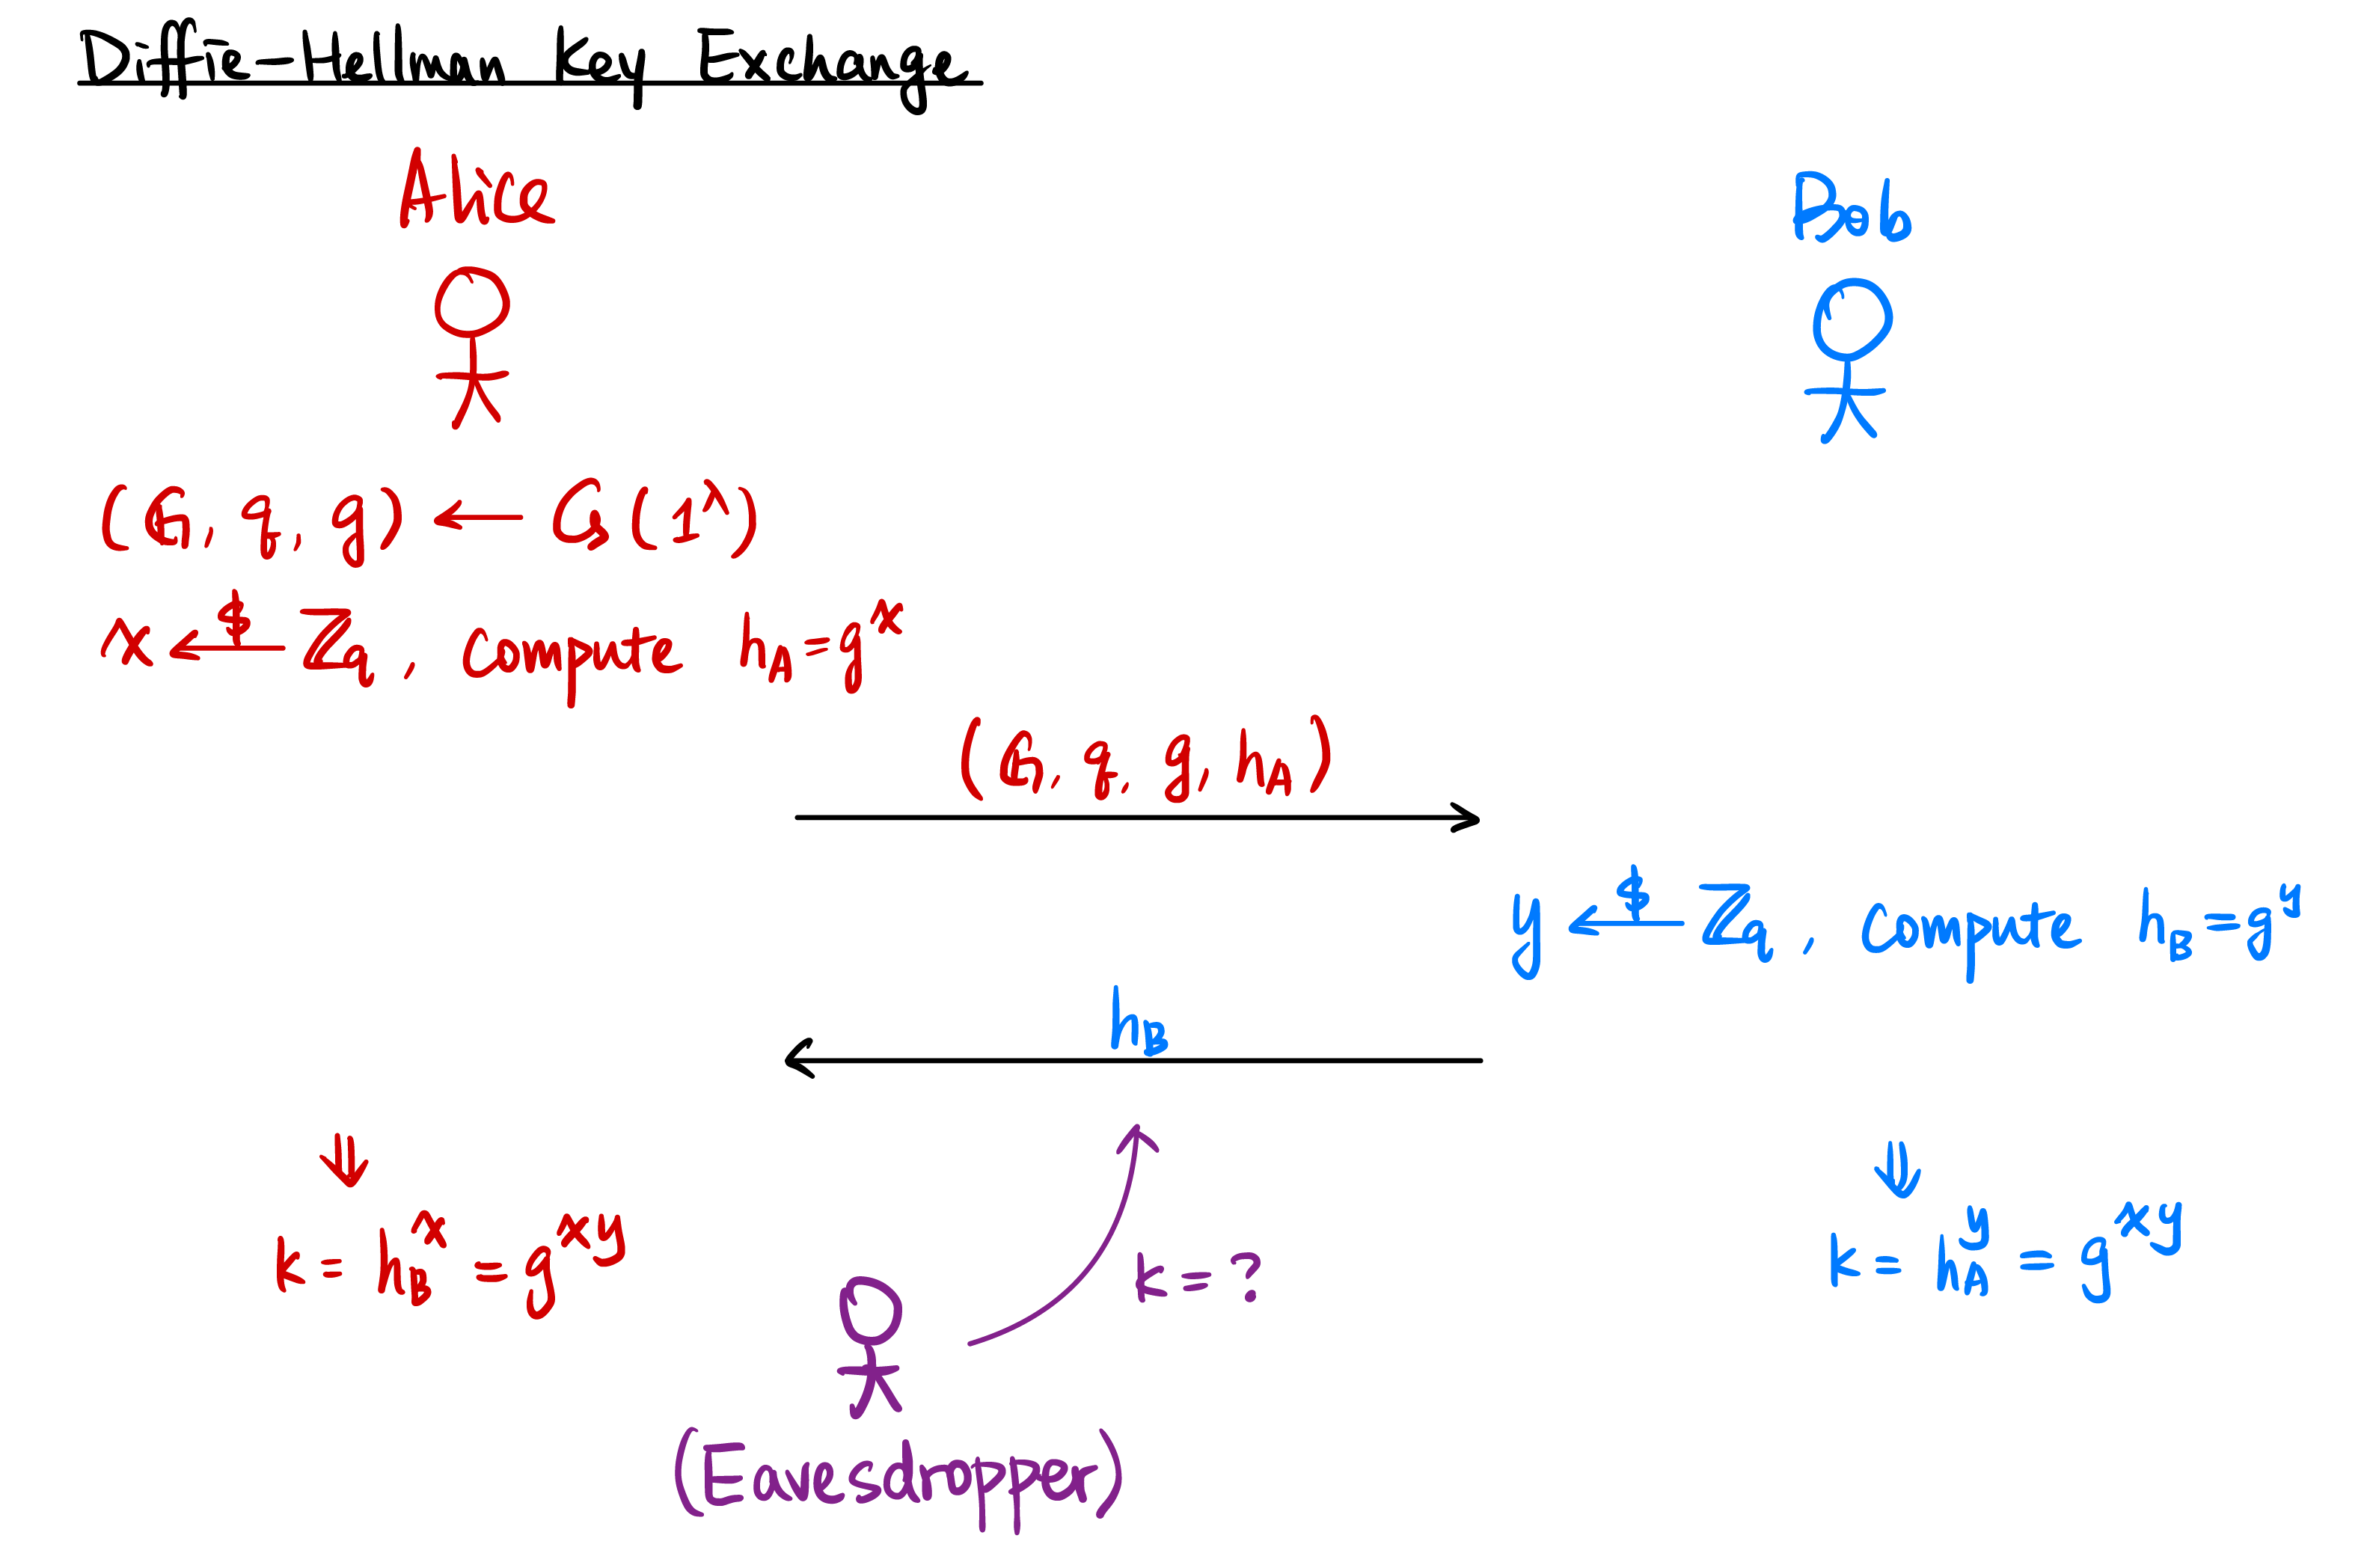
\includegraphics[width=0.8\textwidth]{images/2023-02-02/diffie-hellman.png}
\end{center}

What happens in practice is that parties run Diffie-Hellman key exchange to agree on a shared key. Using that shared key, they run symmetric-key encryption. This gives us efficiency. Additionally, private-key encryptions don't rely on heavy assumptions on the security of protocols (such as the DDH, RSA assumptions).

\subsection{Message Integrity}
Alice sends a message to Bob, how does Bob ensure that the message came from Alice?

\begin{center}
    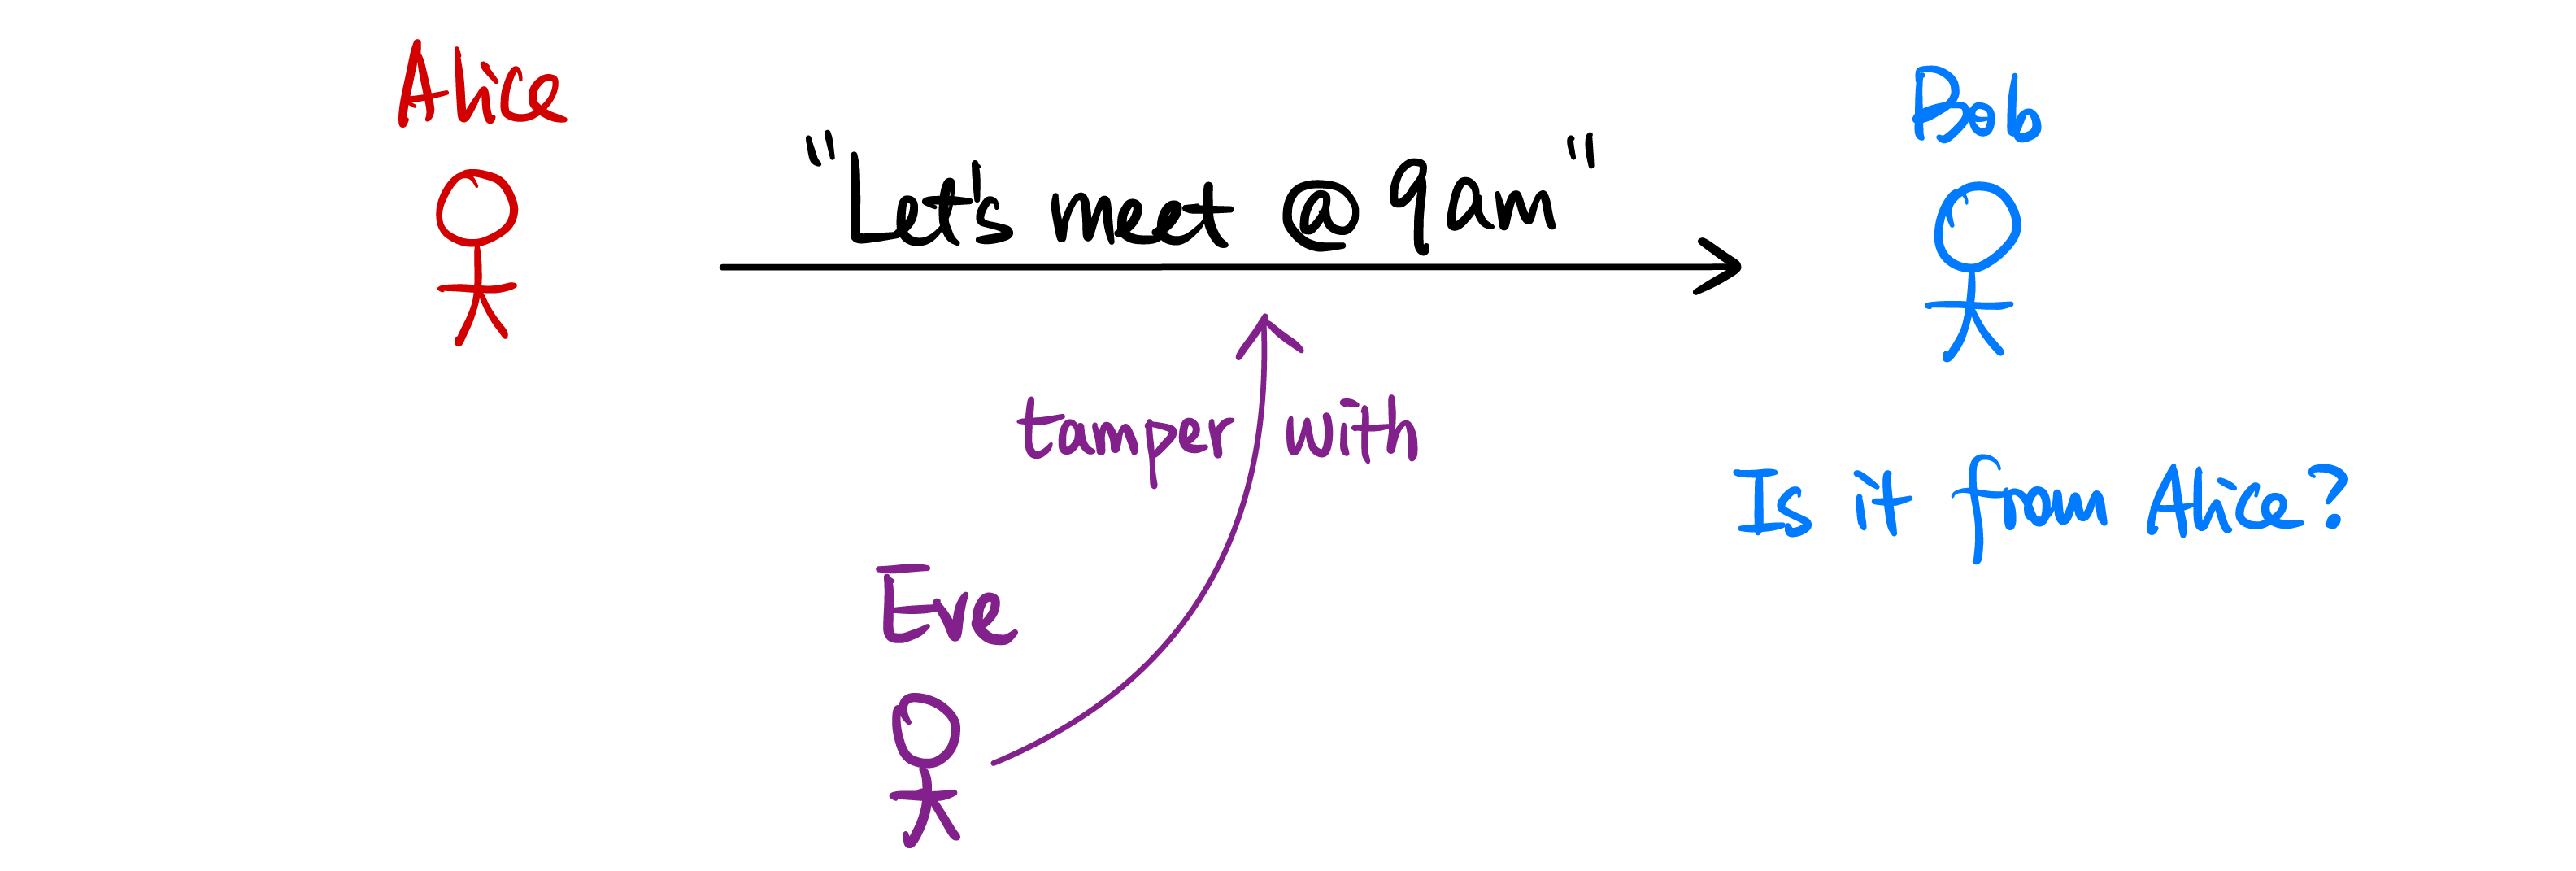
\includegraphics[width=0.8\textwidth]{images/2023-02-02/integrity.png}
\end{center}

We can build up another line of protocols to ensure message integrity. It's similar to encryption, but the parties run 2 algorithms: \emph{Authenticate} and \emph{Verify}.

Using a message $m$, Alice can generate a \emph{tag} or \emph{signature}, and Bob can verify $(m, t)$ is either valid or invalid.

Our adversary has been upgraded to an Eve who can now tamper with messages.

Similarly to encryption, we have symmetric-key and public-key encryption.

Using a shared key $k$, Alice can authenticate $m$ using $k$ to get a tag $k$. Similarly, Bob can verify whether $(m, t)$ is valid using $k$. This is called a Message Authentication Code.

\begin{center}
    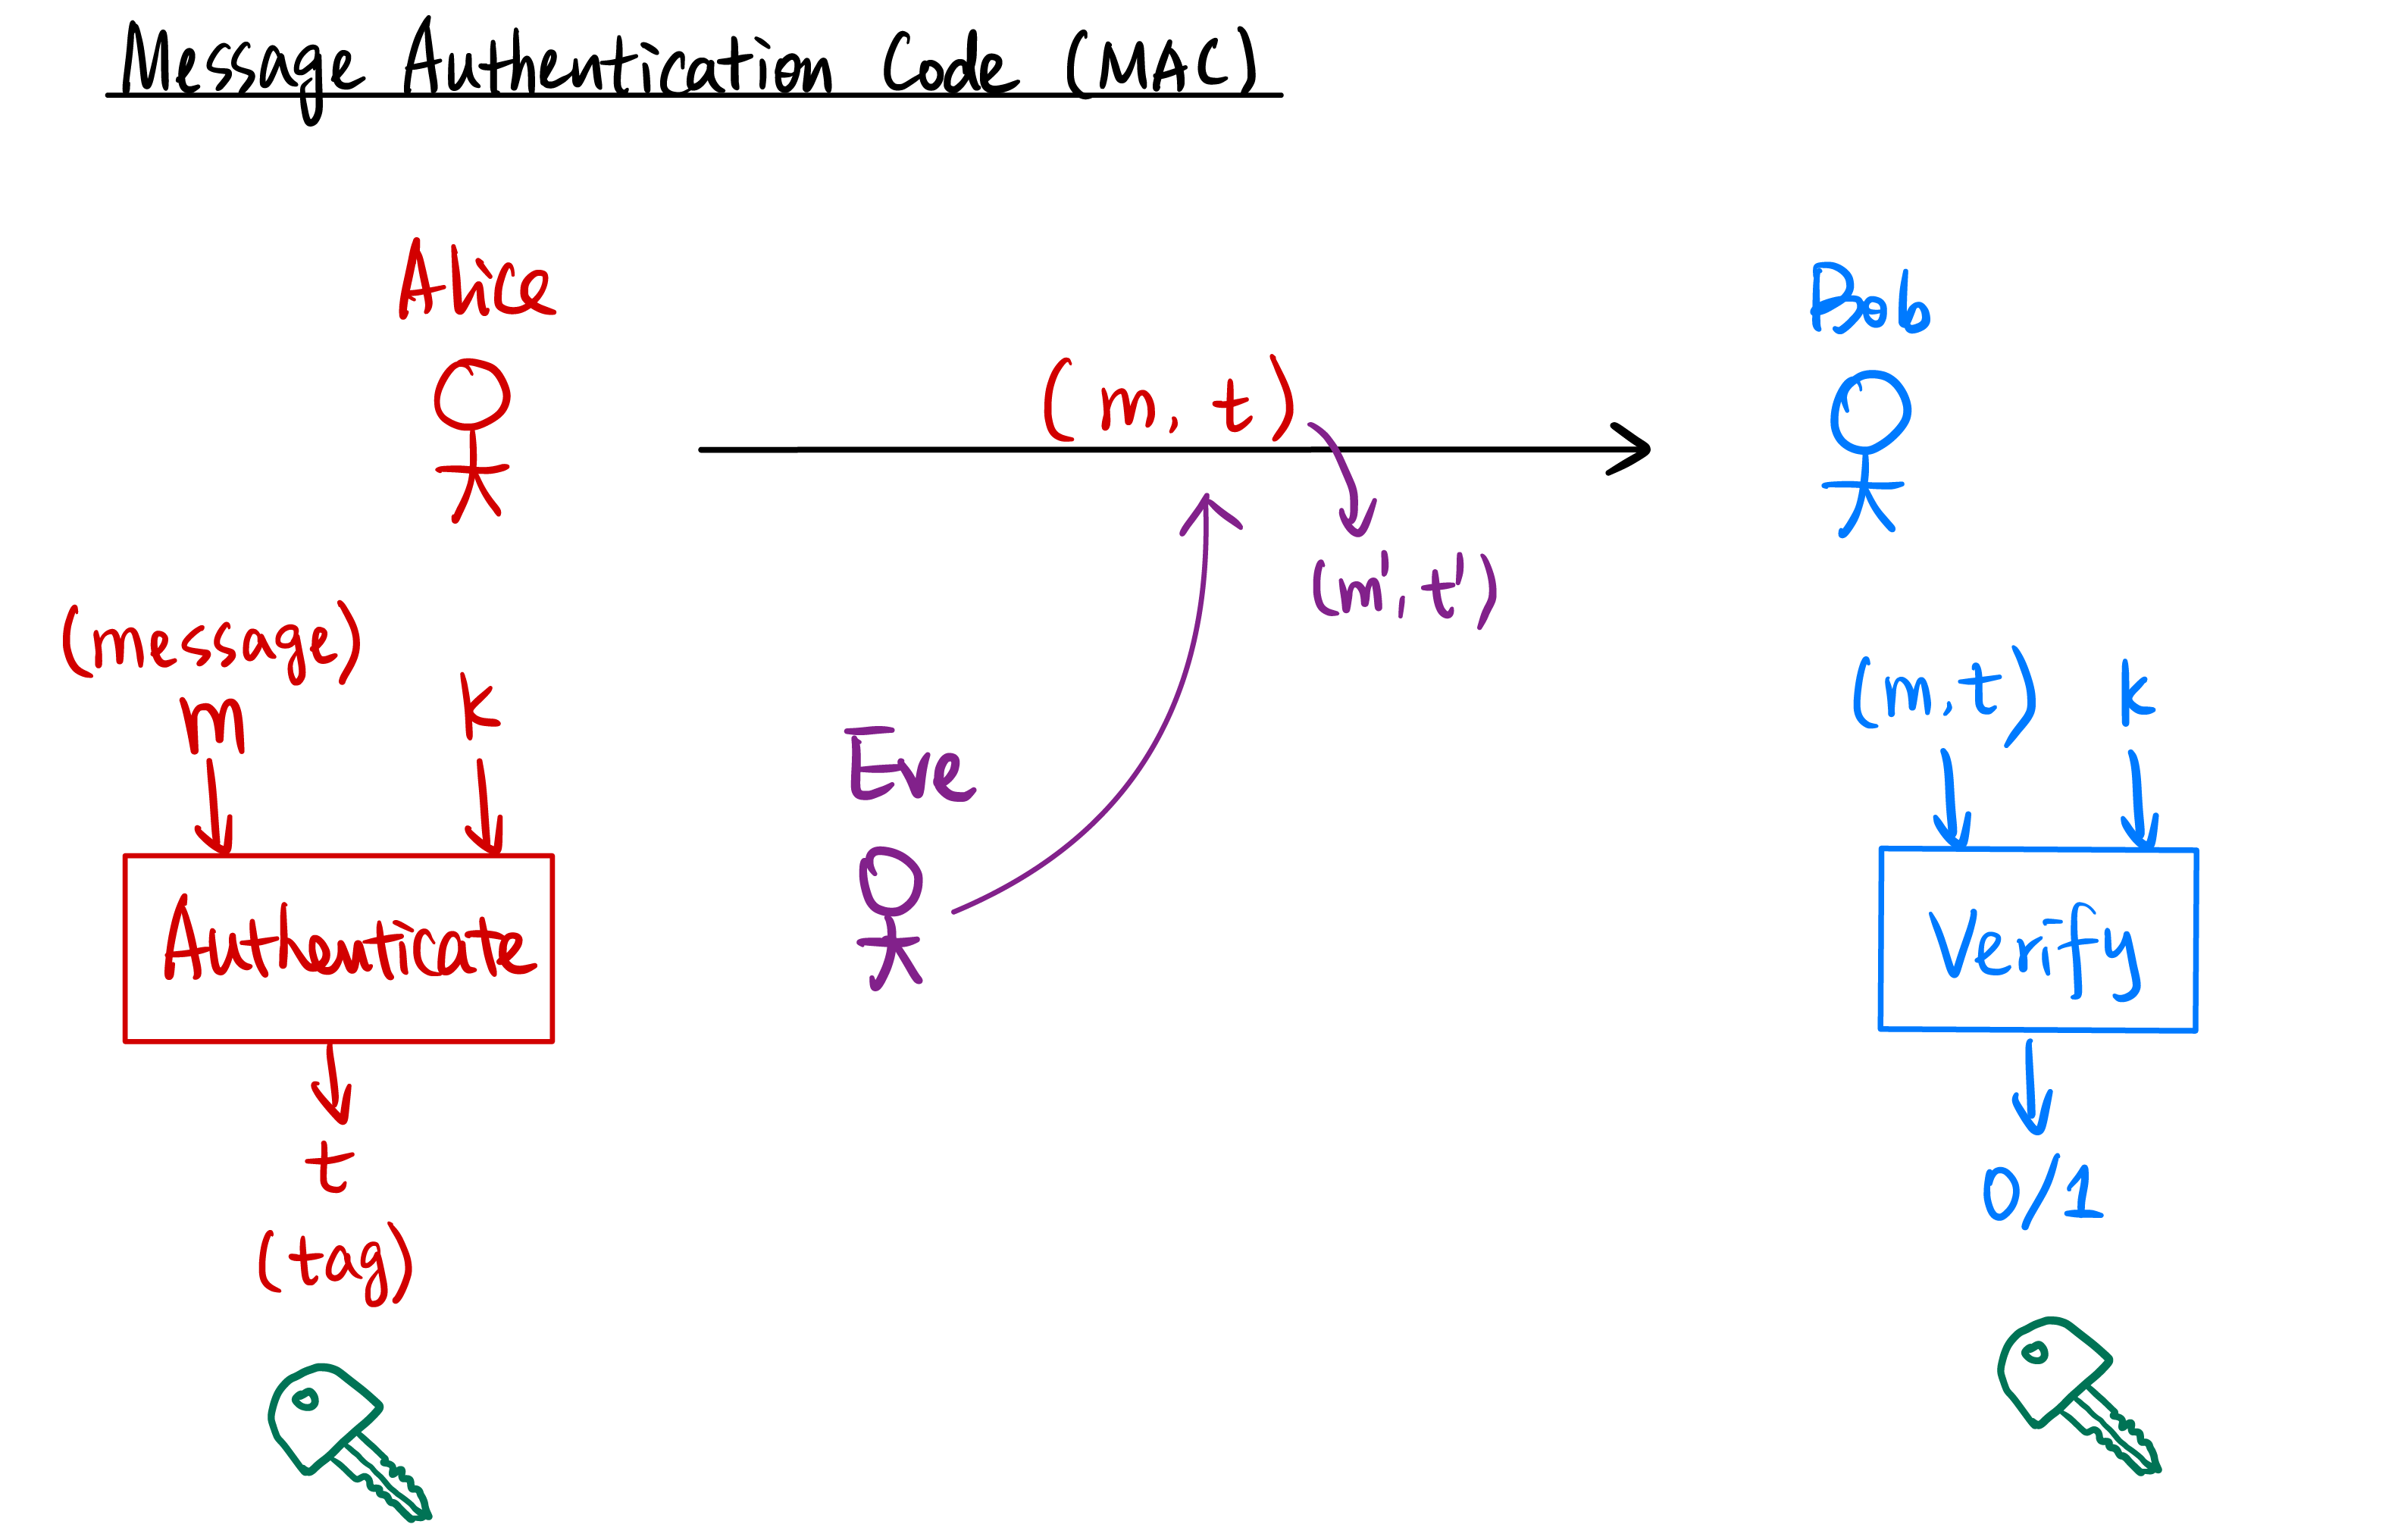
\includegraphics[width=0.8\textwidth]{images/2023-02-02/mac.png}
\end{center}

Using a public key $vk$ (verification key) and private key $sk$ (secret/signing key), Alice can sign a message $m$ using signing key $sk$ to get a \emph{signature} $\sigma$. Bob verifies $(m, \sigma)$ is valid using $vk$. This is called a Digital Signature.

\begin{center}
    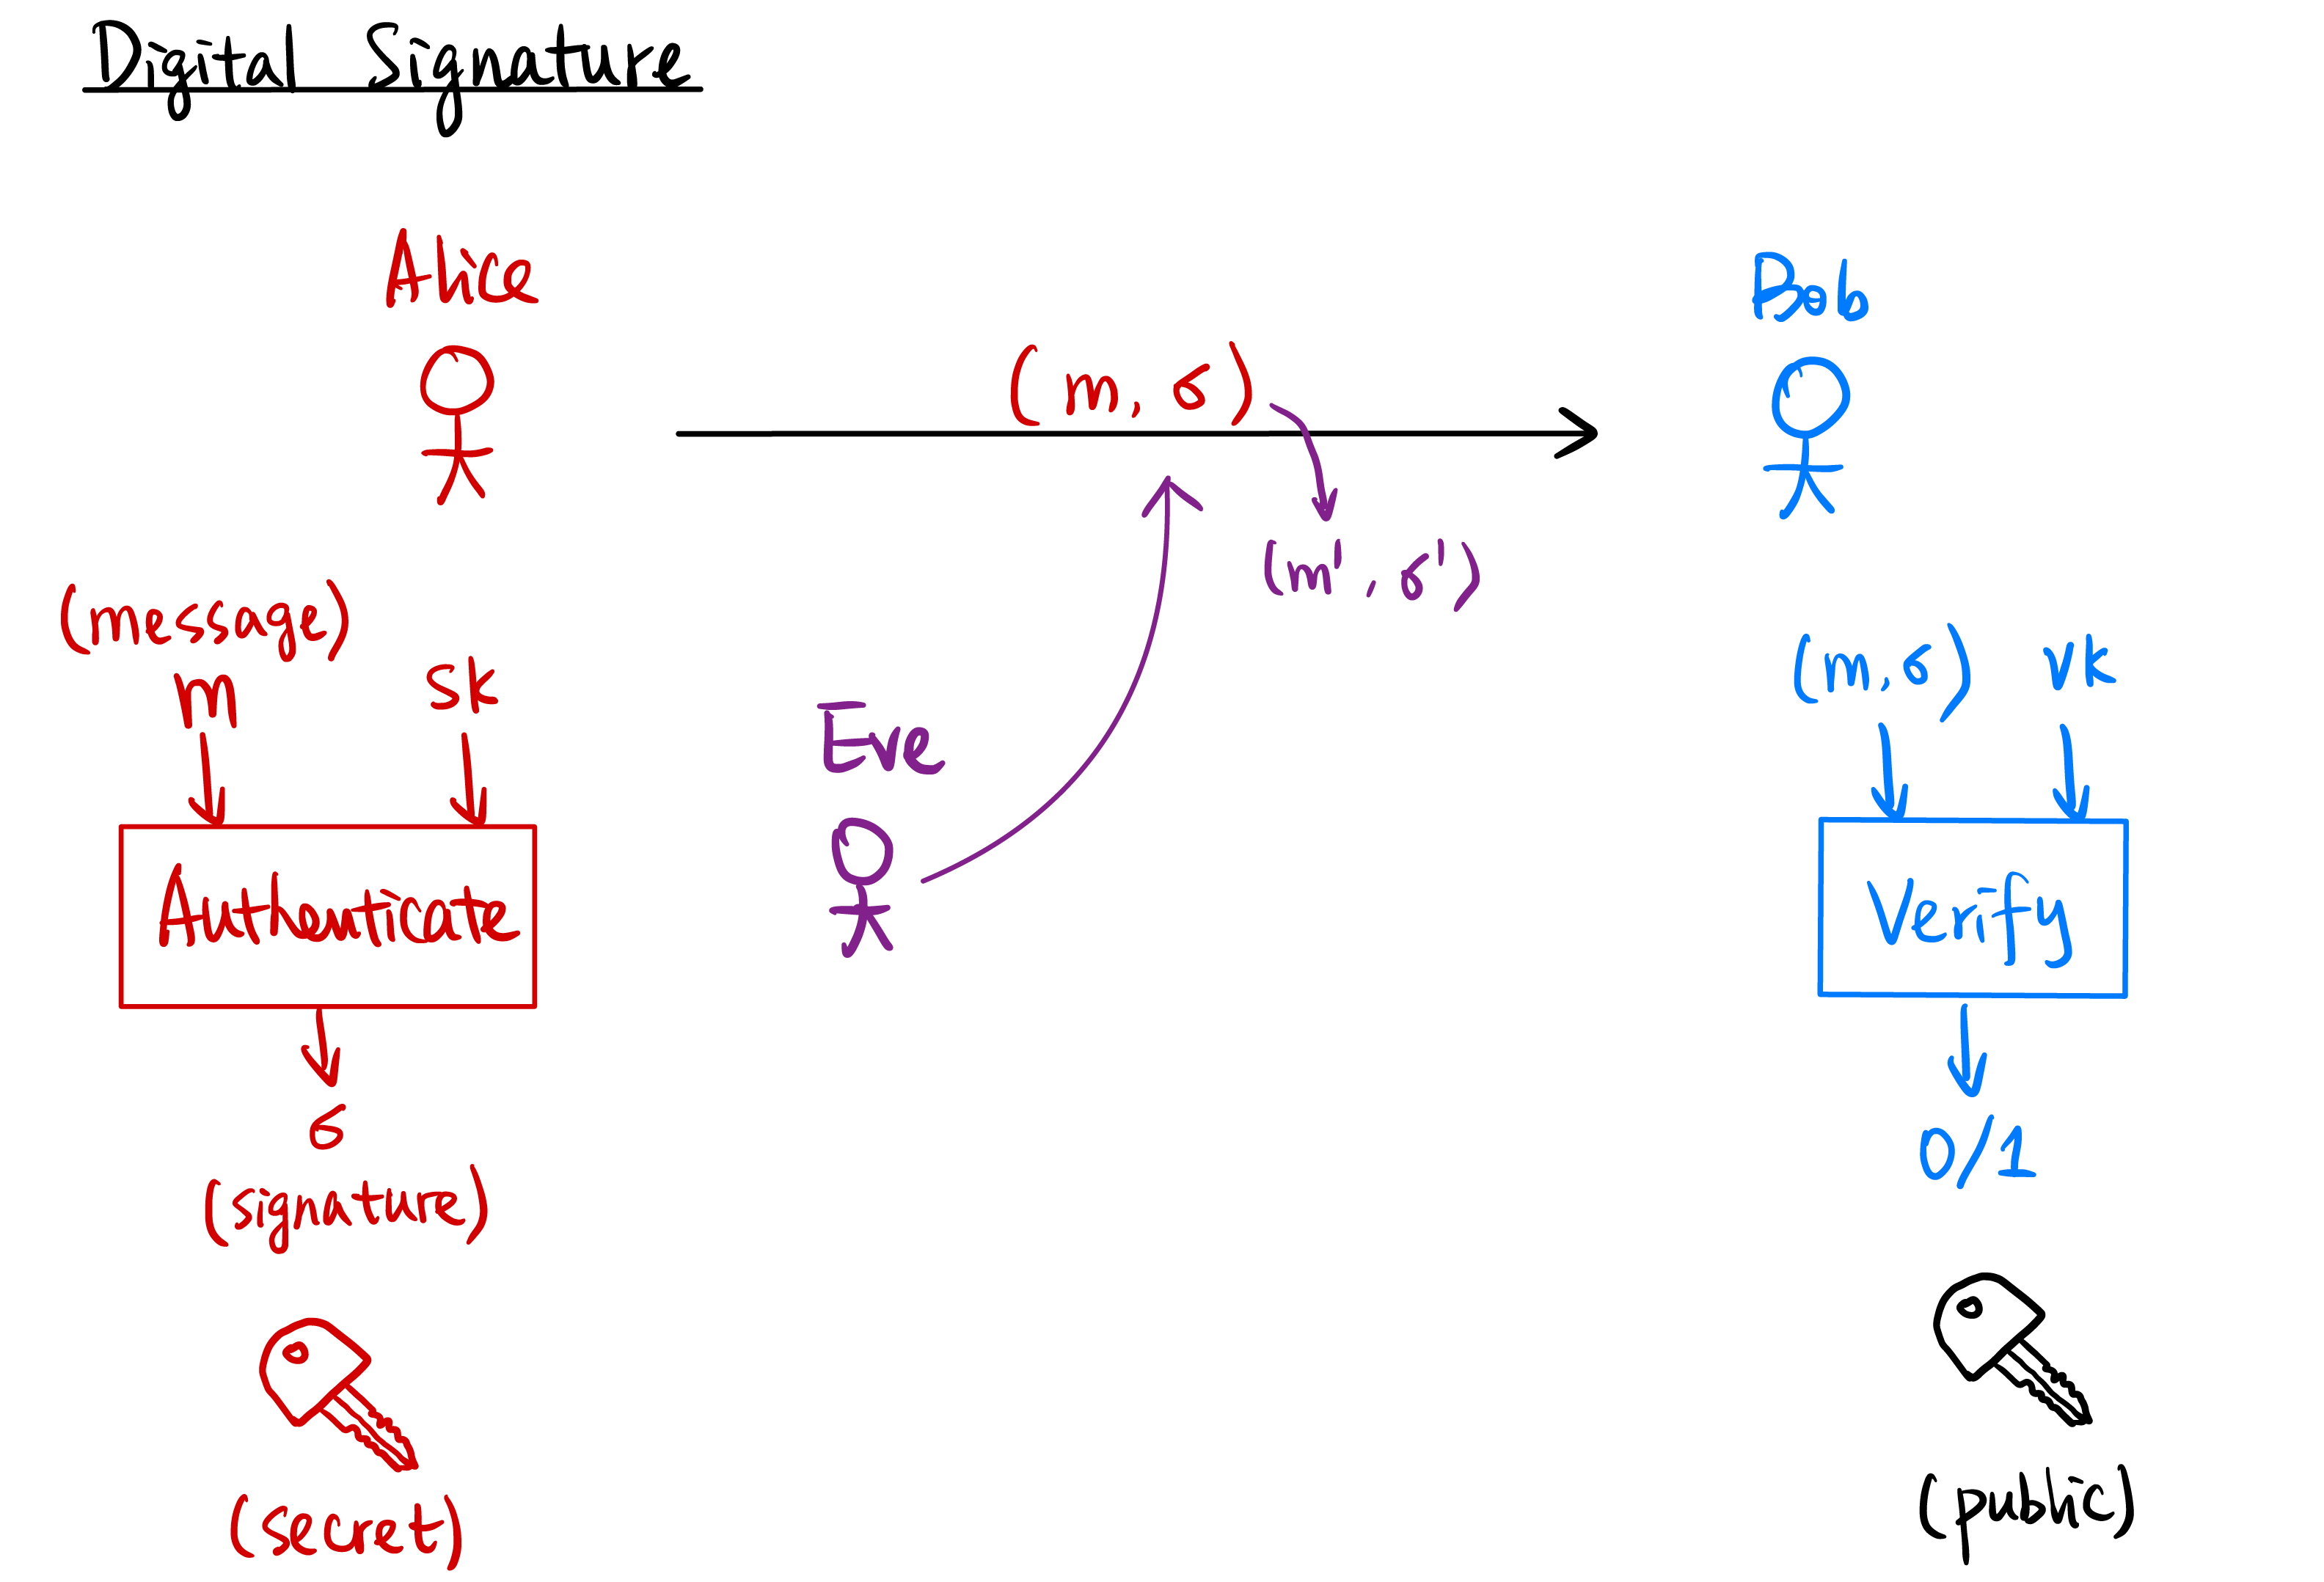
\includegraphics[width=0.8\textwidth]{images/2023-02-02/signature.png}
\end{center}

\subsubsection{Syntax}\label{sec:message-integrity:syntax}
The following is the syntax we use for MACs and digital signatures.

A message authentication code (MAC) scheme consists of $\Pi = (\Gen, \mathsf{Mac}, \mathsf{Verify})$.
\begin{description}
    \item[Generation.] $k\leftarrow \Gen(1^\lambda)$.
    \item[Authentication.] $t \leftarrow \mathsf{Mac}_k(m)$.
    \item[Verification] $0/1 := \mathsf{Verify}_k(m, t)$.
\end{description}

A digital signature scheme consists of $\Pi = (\Gen, \mathsf{Sign}, \mathsf{Verify})$.
\begin{description}
    \item[Generation.] $(sk, vk)\leftarrow \Gen(1^\lambda)$.
    \item[Authentication.] $\sigma \leftarrow \mathsf{Sign}_{sk}(m)$.
    \item[Verification] $0/1 := \mathsf{Verify}_{vk}(m, \sigma)$.
\end{description}

\subsubsection{Chosen-Message Attack}
Similar to chosen-plaintext attack from encryption, we have chosen-message attack security. An adversary chooses a number of messages to generate signatures or tags for. After that, the adversary will try to generate another valid pair of message and tag. We want to make sure that generating a new pair of message and tag is hard.

\begin{center}
    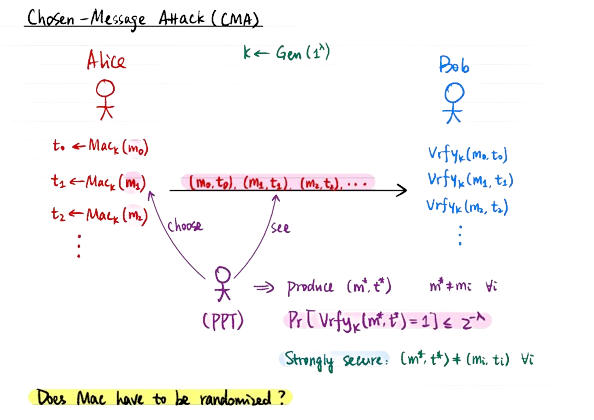
\includegraphics[width=0.8\textwidth]{images/2023-02-02/cma.png}
\end{center}

\subsubsection{Constructions}
Very briefly, we discuss constructions for MAC and digital signatures.

Using block ciphers, we have CBC-MAC. Using a hash function, we have HMAC.

For digital signatures, we have RSA which relies on the RSA assumption, or DSA which relies on discrete-log algorithms. There are also lattice signature schemes for post-quantum digital signatures.
%!TEX root = ../notes.tex
\section{February 7, 2023}
\label{20230207}
\subsection{Message Integrity, \emph{reviewed}}

Last lecture, we discussed methods of authenticating a message. The symmetric-key version is called a MAC (message authentication code), the public-key version is called a digital signature. Let's review what we covered last time.

\subsubsection{Message Authentication Code}
To authenticate a message, Alice will use the private key $k$ to tag a message $m$ with a tag $t$. Bob will verify that $(m, t)$ is valid with key $k$.

\Graphic{images/2023-02-07/mac.png}{0.7}

\subsubsection{Digital Signature}
In the public-key version, Alice has a secret key $sk$ to sign message $m$ with signature $\sigma$. Bob (or anyone) can verify with the public key $pk$ that $(m, \sigma)$ is a valid signature.

\Graphic{images/2023-02-07/ds.png}{0.7}

\subsubsection{Syntax}
Recall the syntax of MAC and digital signatures (see \cref{sec:message-integrity:syntax}).

A message authentication code (MAC) scheme consists of $\Pi = (\Gen, \mathsf{Mac}, \mathsf{Verify})$.
\begin{description}
    \item[Generation.] $k\leftarrow \Gen(1^\lambda)$.
    \item[Authentication.] $t \leftarrow \mathsf{Mac}_k(m)$.
    \item[Verification] $0/1 := \mathsf{Verify}_k(m, t)$.
\end{description}

A digital signature scheme consists of $\Pi = (\Gen, \mathsf{Sign}, \mathsf{Verify})$.
\begin{description}
    \item[Generation.] $(sk, vk)\leftarrow \Gen(1^\lambda)$.
    \item[Authentication.] $\sigma \leftarrow \mathsf{Sign}_{sk}(m)$.
    \item[Verification] $0/1 := \mathsf{Verify}_{vk}(m, \sigma)$.
\end{description}

\subsubsection{Constructions}
We can construct MAC pratically using
\begin{itemize}
    \item Block Cipher: CBC-MAC
    \item Hash Functions: HMAC
\end{itemize}

We can construct digital signatures using
\begin{itemize}
    \item RSA signature: RSA Assumption.
    \item DSA signature: Discrete Log Assumption
    \item Lattice-Based Encryption Schemes (post-quantum secure).
\end{itemize}

\subsection{RSA Signatures}
Our RSA signatures algorithm works very similarly to RSA encryption.

We generate two $n$-bit primes $p, q$. Compute $N:=p\cdot q$ and $\phi(N) = (p-1)(q-1)$. Again choose $e$ with $\gcd(e, \phi(N)) = 1$ and invert $d = e^{-1}\mod\phi(N)$. Given $N$ and a random $y\sampledfrom\ZZ_N^\times$, it's computationally hard to find $x$ such that $x^e\equiv y\mod N$.

Similarly, $sk := d$ and $vk := (N, e)$. To sign, we compute
\[\Sign_{sk}(m) := m^d\mod{N}.\]
To verify, we compute
\[\Verify_{vk}(m, \sigma):= \sigma^e\overset{?}{\equiv}m\mod N.\]

\begin{ques*}
    Are there any security issues with RSA as we have constructed it so far?
\end{ques*}

Thinking back to our definition of chosen-message attack, if Eve knows many messages and signatures, she can compute another pair of valid message and keys. If we have messages
\begin{align*}
    m_0, \sigma_0 & = m_0^d\mod N \\
    m_1, \sigma_1 & = m_0^d\mod N
\end{align*}
We can compute $m^* := m_0\cdot m_1$ and $\sigma^* := \sigma_0 \cdot \sigma_1 = (m_0\cdot m_1)^d\mod N$.

We can do linear combinations of messages, as well as raising messages to arbitrary exponents, and we can get other messages with valid signatures.

There is an easy solution, however. We can hash our message $m$ before we sign, like so
\begin{align*}
    \Sign_{sk}(m)           & := {\color{red}H(}m{\color{red})}^d\mod{N}                         \\
    \Verify_{vk}(m, \sigma) & := \sigma^e\overset{?}{\equiv}{\color{red}H(}m{\color{red})}\mod N
\end{align*}
where $H$ is a hash function\footnote{A hash function is, briefly, a function that produces some random output that is hard to compute the inverse of.}. This is a commonly known technique called `hash-and-sign'.

\subsection{DSA Signatures}
DSA signatures are a bit more involved; they rely on the discrete log assumption and that it is hard to compute discrete logs in $\ZZ_p^\times$ and $\ZZ_q^\times$ a subgroup.

We give this definition using integer groups. There is also ECDSA which uses elliptic curve groups, which is used in cryptocurrencies\footnote{The specific curve used by Bitcoin, for example, is called \textbf{secp256k1}.}. Elliptic curves are much more efficient (especially when chosen correctly) and provide similar security guarantees.

\begin{description}
    \item[$\Gen(1^k)$:] We generate an $n$-bit\footnote{Usually, $2048$.} prime $p$ and an $m$-bit\footnote{Usually, $256$. We assume discrete log in \emph{both} of these groups.} prime $q$ such that $q\mid (p-1)$. We pick a random $\alpha\in\ZZ_p^\times$ such that $g = \alpha^{\frac{p-1}{q}}\mod{p}\neq 1$\footnote{This means that $\langle g\rangle$ has order $q$, a subgroup in $\ZZ_p^{-1}$. $g^q \equiv \alpha^{p-1}\equiv 1\mod{p}$. }

        We pick $x\sampledfrom \ZZ_q^\times$ and compute $h = g^x\mod{p}$.

        Our verification key is $vk := (p, q, g, h)$ and our signing key is $sk = x$.

    \item[$\Sign_{sk}(m)$:] Sample $y \sampledfrom \ZZ_q^\times$, compute $r = (g^y\mod{p})\mod{q}$. Compute $s = y^{-1}\cdot(H(m) + x\cdot r)\mod{q}$ and $\sigma := (r, s)$.

    \item[$\Verify_{vk}(m, \sigma)$:] We can compute
        \begin{align*}
            w   & = s^{-1}\mod{q}       \\
            u_1 & = H(m)\cdot w \mod{q} \\
            u_2 & = r\cdot w\mod{q}
        \end{align*}
        and verify $r\overset{?}{=}\left( g^{u_1}\cdot h^{u_2}\mod{p} \right)\mod{q}$.
\end{description}

\subsection{Authenticated Encryption}
Generally, Alice and Bob will first perform a Diffie-Hellman key exchange, then use that shared key to conduct Symmetric-Key Encryption.

\Graphic{images/2023-02-07/practice.png}{0.6}

In reality, we want to achieve both message secrecy and integrity \emph{at the same time}. For this, we can introduce Authenticated Encryption.

Our security definition is that our adversary can see the encryptions of many messages $m_0, m_1, m_2$. We want \textbf{CPA security}: given an encryption of either $m_0, m_1$, our adversary cannot distinguish between encryptions of the two. \emph{Additionally}, we want the property of \textbf{unforgeability}, that our adversary cannot generate a $c^*$ that is a valid encryption, such that $\Dec_{k}(c^*)\neq m_i$ for any $i$.

\Graphic{images/2023-02-07/ae.png}{0.8}

Now that we have two new primitives, we can construct Authenticated Encryption schemes.

\subsubsection{Encrypt-and-MAC?}
Given a CPA-secure SKE scheme $\Pi_1(\Gen_1, \Enc_1, \Dec_1)$ and a CMA-secure MAC scheme $\Pi_2 = (\Gen_2, \Mac_2, \Verify_2)$.

We construct an AE scheme $\Pi = (\Gen, \Enc, \Dec)$ by composing encryption and MAC. We encrypt the plaintext and also compute the MAC the \emph{plaintext}.

\Graphic{images/2023-02-07/encrypt-and-mac.png}{0.3}

\begin{description}
    \item[$\Gen(1^\lambda)$:] $k_1:=\Gen_1(1^\lambda)$, $k_2:=\Gen_2(1^\lambda)$, output $(k_1, k_2)$.

    \item[$\Enc(m)$:] To encrypt, we first encrypt ciphertext $c_1 := \Enc_1(k_1, m)$ and sign message (in plaintext) $t_2 := \Mac_2(k_2, m)$ and output $(c_1, t_2)$.

    \item[$\Dec(m)$:] We have ciphertext $c = (c_1, t_2)$. Our message is $m:=\Dec_1(k_1, c_1)$, and our verification bit $b := \Verify_1(k_2, (m, t_2))$. If $b = 1$, output $m$, otherwise we output $\bot$.
\end{description}

\begin{ques*}
    Is this scheme secure? Assuming the CPA-secure SKE scheme and CMA-secure MAC scheme, does this give us both CPA-security and unforgeability?
\end{ques*}

MAC gives you \emph{unforgeability}---it doesn't even try to hide the message at all. It's possible that the MAC scheme reveals the message in the clear. For example, we might have a MAC scheme that includes the message in the signature \emph{in the clear} (which is still secure)!

Since MAC doesn't try to hide the message. If our MAC reveals something about our message, our composed scheme $\Pi$ doesn't give us CPA-security. You might still be able to infer something about the message.

We try something else\dots

\subsubsection{Encrypt-then-MAC}
We encrypt first, then we MAC on the \emph{ciphertext}.

\Graphic{images/2023-02-07/encrypt-then-mac.png}{0.3}

\begin{description}
    \item[$\Gen(1^\lambda)$:] $k_1:=\Gen_1(1^\lambda)$, $k_2:=\Gen_2(1^\lambda)$, output $(k_1, k_2)$.

    \item[$\Enc(m)$:] To encrypt, we first encrypt ciphertext $c_1 := \Enc_1(k_1, m)$ and sign message (in ciphertext) $t_2 := \Mac_2(k_2, {\color{red} c_1})$ and output $(c_1, t_2)$.

    \item[$\Dec(m)$:] We have ciphertext $c = (c_1, t_2)$. Our message is $m:=\Dec_1(k_1, c_1)$, and our verification bit $b := \Verify_1(k_2, ({\color{red} c_1}, t_2))$. If $b = 1$, output $m$, otherwise we output $\bot$.
\end{description}

You can prove that Encrypt-then-MAC schemes are CPA-secure and unforgeable.

\subsubsection{MAC-then-Encrypt}
Similarly, we can also MAC first, encrypt the entire ciphertext and tag concatenated.

\Graphic{images/2023-02-07/mac-then-encrypt.png}{0.3}

\begin{description}
    \item[$\Gen(1^\lambda)$:] $k_1:=\Gen_1(1^\lambda)$, $k_2:=\Gen_2(1^\lambda)$, output $(k_1, k_2)$.

    \item[$\Enc(m)$:] To encrypt, we first encrypt ciphertext $c_1 := \Enc_1(k_1, m)$ and sign message (in plaintext) $t_2 := \Mac_2(k_2, {\color{red} m||t_2})$ and output $(c_1, t_2)$.

    \item[$\Dec(m)$:] We have ciphertext $c = (c_1, t_2)$. Our message is ${\color{red} m||t_2}:=\Dec_1(k_1, c_1)$, and our verification bit $b := \Verify_1(k_2, (m, t_2))$. If $b = 1$, output $m$, otherwise we output $\bot$.
\end{description}

\begin{ques*}
    Is this secure?
\end{ques*}

This doesn't satisfy a stronger security definition called Chosen Ciphertext Attack (CCA) security. We might be able to forge ciphertexts that decrypt to valid message and tags.

\subsubsection{Chosen Ciphertext Attack Security}
On top of CMA security, the adversary can now request Alice to decrypt ciphertexts $c_0, c_1, \dots$.

\Graphic{images/2023-02-07/cca.png}{0.7}

We can prove that MAC-then-Encrypt is not CCA secure.

The moral of this is that \textbf{you should always use Encrypt-then-MAC.}

\subsection{A Summary So Far}
To summarize, here's all we've covered so far:
\begin{center}
    \begin{tabular}{@{}lll@{}}
        \toprule
                                      & \textbf{Symmetric-KePy}                                                                & \textbf{Public-Key}                                                                   \\ \midrule
        \textbf{Message Secrecy}      & \begin{tabular}[c]{@{}l@{}}Primitive: SKE\\ Construction: Block Cipher\end{tabular}    & \begin{tabular}[c]{@{}l@{}}Primitive: PKE\\ Constructions: RSA/ElGamal\end{tabular}   \\ \midrule
        \textbf{Message Integrity}    & \begin{tabular}[c]{@{}l@{}}Primitive: MAC\\ Constructions: CBC-MAC/HMAC\end{tabular}   & \begin{tabular}[c]{@{}l@{}}Primitive: Signature\\ Constructions: RSA/DSA\end{tabular} \\ \midrule
        \textbf{Secrecy \& Integrity} & \begin{tabular}[c]{@{}l@{}}Primitive: AE\\ Construction: Encrypt-then-MAC\end{tabular} &                                                                                       \\ \midrule
        \textbf{Key Exchange}         &                                                                                        & Construction: Diffie-Hellman                                                          \\ \midrule
        \textbf{Important Tool}                & \begin{tabular}[c]{@{}l@{}}Primitive: Hash function\\ Construction: SHA\end{tabular}   &                                                                                       \\ \bottomrule
    \end{tabular}
\end{center}



\subsection{Hash Function}
A hash function is a public function
\[H: {0, 1}^*\to {0, 1}^n\]
where $n$ is order $\Theta(\lambda)$.

\Graphic{images/2023-02-07/hash.png}{0.5}

We want our hash function to be collision-resistant. That is, it's computationally hard to find $x, y\in\left\{ 0, 1 \right\}^*$ such that $x\neq y$ yet $H(x) = H(y)$ (which is called a collision).

How might one find a collision for function $H: \{ 0, 1 \}^*\to \{ 0, 1 \}^n$. We can try $H(x_1), H(x_2), \dots, H(x_q)$.

If $H(x_1)$ outputs a random value, ${0, 1}^n$, what is the probability of finding a collision?

If $q = 2^n + 1$, our probability is exactly $1$ (by pigeon-hole). If $q = 2$, our probability is $\frac{1}{2^\lambda}$ (we have to get it right on the first try). What $q$ do we need for a `reasonable' probability?

\begin{remark*}
    This is related to the birthday problem. If there are $q$ students in a class, assume each student's birthday is a random day $y_i\sampledfrom [365]$. What is the probability of a collision? $q = 366$ gives $1$, $q = 23$ gives around $50\%$, and $q = 70$ gives roughly $99.9\%$.

    We can apply this trick to our hash function. If $y_i\sampledfrom [N]$, then $q = N+1$ gives us $100\%$, but $q = \sqrt{N}$ gives $50\%$ probability.
\end{remark*}

Knowing this, we want $n = 2\lambda$ (output length of hash function). If $\lambda = 128$, we want $n$ to be around $256$.

\subsubsection{Random Oracle Model}
Another way to model a hash function is the \emph{Random Oracle Model}. We think of our hash function to be an oracle (in the sky) that can \emph{only} take input and a random output (and if you give it the same input twice, the same output).

\Graphic{images/2023-02-07/oracle.png}{0.5}

There are proofs that state that no hash functions can be a random oracle. There are schemes that can be secure in the random oracle model, but are not using hash functions\footnote{Some constructions don't rely on this model.}.

In reality, hash functions are \emph{about as good as}\footnote{But can never be\dots} random oracles. Thinking of our hash functions as random oracles gives us a good intuitive understanding of how hash functions can be used in our schemes.

In this model, the best thing that an attacker can do is to try inputs and query for outputs.

\subsubsection{Constructions for Hash Function}
\begin{description}
    \item[MDS.] Output length $128$-bit. Best known attack is in $2^{16}$. A collision was found in 2004.
\end{description}
And we also have Secure Hash Functions (SHA), founded by NIST.
\begin{description}
    \item[SHA-0.] Standardized in 1993. Output length is 160-bit. Best known attack is in $2^{39}$.
    \item[SHA-1.] Standardized in 1995. Output length is $160$-bit. Best known attack is in $2^{63}$, and a collision \emph{was} found in 2017.
    \item[SHA-2.] Standardized in 2001. Output length of 224, 256, 284, 512-bit. The most commonly used is SHA-256.
    \item[SHA-3.] There was a competition from 2007-2012 for new hash functions. SHA-3 was released in 2015, and has output length 224, 256, 2384, 512-bit. This is \emph{completely different} from SHA-2.
\end{description}

\begin{remark*}
    The folklore is that during a session at a cryptography conference, a mathematician, Xiaoyun Wang, presented slide-after-slide of attacks on MDS and SHA-0, astounding the audience.
\end{remark*}
%!TEX root = ../notes.tex
\section{February 9, 2023}
\label{20230209}

\emph{Logistics:} Please let us know if you have outstanding Ed or Gradescope issues!

\subsection{Hash Functions, \emph{continued}}
Recall that we defined a hash function to be a function for which it is computationally hard to find a collision. That is, finding two distinct strings $x, y$ such that $H(x) = H(y)$ is computationally difficult.

\Graphic{images/2023-02-09/hash.png}{0.4}

One model that we sometimes use to facilitate our analysis is the random oracle model. We assume our hash function is a random oracle `in the sky'that produces random hashes.

By guessing, analyzing it via the birthday problem, we require time approximately $\sqrt{n}$.

\Graphic{images/2023-02-09/hash-oracle.png}{0.4}

\subsubsection{Constructions}

The hash function constructions that are still in practice (and unbroken) are SHA-2 and SHA-3.

\subsubsection{Applications}

\begin{description}
    \item[HMAC.] We can use a hash function to conduct a MAC. Computing a tag involves computing the hash function on the key appended to the message ($k||m$). It is computationally difficult to find another $k || m'$ that produces the same hash. This is a scheme that looks like
        \[\Mac_k(m) = H(k||m).\]

        However, an adversary could potentially attach some additional $s$ to $m$ to produce $m' = m||s$ such that they can easily compute $\mathsf{tag}' = H(\mathsf{tag}||s)$. This is due to the Merkle-Damgård construction of SHA-2, which associatively tags blocks of the message one-by-one.

        \Graphic{images/2023-02-09/md.png}{0.4}

        Therefore, in practice, we use a nested MAC like
        \[\Mac_k(m) = H(k||H(k||m))\]
        and just to be sure (that we're not reusing the key), we produce $k_1, k_2$ as such
        \[\mathsf{HMAC}_k(m) = H(k_1||H(k_2||m))\]
        such that $k_1 = k\oplus \mathsf{opad}$ and $k_2 = k\oplus\mathsf{ipad}$, some one-time pads.

    \item[Hash-and-Sign.] There are some other applications of a hash function. We've seen before with RSA that we want to Hash-and-Sign, removing any homomorphism that an adversary could exploit. Additionally, this allows us to sign larger messages since they are constant size after hashing.

    \item[Password Authentication.] Another application is password authentication. Instead of storing plaintext passwords on servers, websites can store a hash of the password instead. This means that the passwords are not compromised even if the server is compromised.

    \item[Deduplicate Files.] We can also use hash functions to deduplicate files. We can hash two files to produce identifiers $h_1$ and $h_2$. If $h_1\neq h_2$, this implies $D_1\neq D_2$. If $h_1 = h_2$, it almost always\footnote{If they are not equal, we've found a collision for our hash function, which is extremely unlikely.} implies that $D_1 = D_2$.

    \item[HKDF (Key Derivation Function).] We can derive more keys from a shared key, essentially using a hash function as a pseudorandom generator (PRG).

        For example, if there is $g^{ab}$ shared key, we can do
        \[\mathsf{HMAC}(g^{ab}, \textsf{salt})\]

        Using a random seed, and adding a public deterministic salt $G$, we can generate a random\footnote{Computationally random, because if our computational power were to be unbounded, we can try all strings.} string.

        \Graphic{images/2023-02-09/hkdf.png}{0.8}

        Given a hash function $H$, we can generate a PRG easily for any length string by generating
        \begin{align*}
            \mathsf{seed}\sampledfrom \{0, 1\}^\lambda \longrightarrow & H(\mathsf{seed}||00\cdots 00) \\
                                                                       & H(\mathsf{seed}||00\cdots 01) \\
                                                                       & H(\mathsf{seed}||00\cdots 10) \\
                                                                       & \qquad\qquad \vdots
        \end{align*}

        We can take a bit of randomness (like the way we move our mouse, type keyboard, system properties) and generate our seed.

    \item[Fast Membership Proof (Merkle Tree).] Using hash functions, we can generate Merkle Trees to prove membership. In blockchains, this is equivalent to checking if a transaction occurred.

    \item[SKE Scheme?] Could we use this to encrypt? If we have a secret key $k\sampledfrom\{0, 1\}^\lambda$, can we just encrypt by
        \[\Enc_k(m) = H(k||m)\]
        Well, we can't decrypt for one without having unbounded computational power. If our plaintext $m$ comes from a small set, like $\{0, \dots, 10\}$, we could decrypt properly. However, this is not CPA-secure, since the adversary could just query for all the messages.

        \begin{remark}
            In general, all deterministic encryption schemes are not CPA-secure.
        \end{remark}
\end{description}

\subsection{Putting it Together: Secure Communication}
This is essentially what we want to do in the second project.

We use Diffie-Hellman Key Exchange between Alice and Bob to get shared $g^{ab}$. Hashing the shared key using an HKDF, we can get shraed key $k = (k_1, k_2)$ (one for AES one for HMAC). Then, they perform authenticated encryption, namely Encrypt-then-MAC.

\begin{ques*}
    Are there any issues with this scheme?
\end{ques*}
An Eve could pretend to be Alice to Bob and Bob to Alice, fudging up their shared keys. This is called a \emph{Man-in-the-Middle} attack.

\subsubsection{Diffie-Hellman Ratchet}
What if a secret key gets leaked, or cracked? One simple way to fix this is to perform a Diffie-Hellman key exchange on every message. However, this incurs additionall communications costs.

Here's another idea: with every new message (when the direction of communications shifts), the party sending the message sends a new Diffie-Hellman public key for themselves. For example, if Bob is sending a message to Alice and he knows Alice's public key $g^{a_1}$ and his previous secret was $b_1$ (hence shared $g^{a_1b_1})$, Bob will generate new key $b_2, g^{b_2}$ and encrypt using $g^{a_1b_2}$, sending $g^{b_2}$ as public to Alice. Alice can recompute the shared key before decrypting.

\Graphic{images/2023-02-09/dh-ratchet.png}{0.7}

This is the protocol used in the Signal messaging app, and is what you will implement for Project 1.

\begin{ques*}
    What if $k_1$ is leaked?
\end{ques*}
We might have leaked one key, but the other keys are still computationally hard to compute. $k_1=g^{a_1b_1}$ is known, but it's equivalent to DDH to compute $g^{a_1b_2}$ or other keys.

\begin{ques*}
    What if $b_1$ is leaked?
\end{ques*}
We can compute key $k_1=g^{a_1b_1}$ and $k_2=g^{a_2b_1}$, but no further keys are leaked, and the next round of communications (after Bob refreshes his private key $b_2$) is still secure.

\subsection{Block Cipher}
To summarize, here's what we've seen so far (this table should be familiar):
\begin{center}
    \begin{tabular}{@{}lll@{}}
        \toprule
                                      & \textbf{Symmetric-Key}                                                                               & \textbf{Public-Key}                                                                   \\ \midrule
        \textbf{Message Secrecy}      & \begin{tabular}[c]{@{}l@{}}Primitive: SKE\\ Construction: \boxed{\textbf{Block Cipher}}\end{tabular} & \begin{tabular}[c]{@{}l@{}}Primitive: PKE\\ Constructions: RSA/ElGamal\end{tabular}   \\ \midrule
        \textbf{Message Integrity}    & \begin{tabular}[c]{@{}l@{}}Primitive: MAC\\ Constructions: CBC-MAC/HMAC\end{tabular}                 & \begin{tabular}[c]{@{}l@{}}Primitive: Signature\\ Constructions: RSA/DSA\end{tabular} \\ \midrule
        \textbf{Secrecy \& Integrity} & \begin{tabular}[c]{@{}l@{}}Primitive: AE\\ Construction: Encrypt-then-MAC\end{tabular}               &                                                                                       \\ \midrule
        \textbf{Key Exchange}         &                                                                                                      & Construction: Diffie-Hellman                                                          \\ \midrule
        \textbf{Important Tool}       & \begin{tabular}[c]{@{}l@{}}Primitive: Hash function\\ Construction: SHA\end{tabular}                 &                                                                                       \\ \bottomrule
    \end{tabular}
\end{center}
The only thing we haven't seen thus far is a block cipher. We first start with the definitions.

We saw earlier that a Pseudorandom Generator (PRG) produces a string that looks random. We also have Pseudorandom Functions (PRF), which are `random-looking' functions.

\subsubsection{Pseudorandom Function (PRF)}

Our Pseudorandom Function $F$ is a keyed function\footnote{In deterministic polynomial-time.} $F : \{0, 1\}^\lambda\times \{0, 1\}^n\to\{0, 1\}^m$, $F$ will take key $k$ and input $x$ to produce output $y$, $F(k, x) = y$.

Without knowing our key $k$, $F_k$ is computationally indistinguishable from some random $f\sampledfrom\{F\mid F\{0, 1\}^n\to \{0, 1\}^m\}$.

\Graphic{images/2023-02-09/prf.png}{0.8}

We have $2^\lambda$ possible $F_k$'s, and we have $(2^m)^{2^n}$ possible functions $f$. A computationally unbounded adversary could try all possible functions and distinguish our function, since $F_k$ lives in a subset of the space of $f$. However, in reality, we can assume that $F_k$ is computationally indistinguishable from any generic function.

\subsubsection{Pseudorandom Permutation (PRP)}

A further assumption is that our function is a bijection. $F_k$ is a keyed function from $F_k : \{0, 1\}^n\to\{0, 1\}^n$. We still have $2^\lambda$ possible $F_k$'s since there are $2^\lambda$

\Graphic{images/2023-02-09/prp.png}{0.8}

\begin{ques*}
    Again, how many possible $f$'s are there?
\end{ques*}
Our first string has $2^n$ choices to map to, our second choice has $2^n - 1$, so there are
\[(2^n)(2^n-1)(2^n-2)\cdots 1 = 2^n!\]

Still, this is a much larger number than $2^\lambda$, so we still make a computational assumption that our keyed function $F_k$ is still computationally indistinguishable from a random function $f$.

\subsubsection{Block Cipher Definition}
A block cipher is a function
\[F : \{0, 1\}^\lambda\times \{0, 1\}^n\to \{0, 1\}^n\]
where $\lambda$ is the key length and $n$ is the block length. A block cipher is assumed to be a pseudorandom permutation (PRP).

Our practical construction is the Advanced Encryption Standard (AES).
\begin{itemize}
    \item Our key and block sizes are $\lambda = n = 128$.
    \item This was standardized by NIST in 2001.
    \item There was a competition from 1997-2000 to come up with a block cipher scheme. It is said that the end of the competition, competitors were simply trying to attack each other's schemes. AES was eventually selected for its efficiency.
    \item Before AES, we used the Data Encryption Standard (DES) with $\lambda = 56$ and $n = 64$. The best attack is \emph{still} a brute-force search, but key and block lengths are relatively fixed (cannot be extended).
\end{itemize}

Currently, the best attack for AES is still a brute-force search, which takes time $2^{128}$.

\subsubsection{Block Cipher Modes of Operation}
We have block cipher
\[F : \{0, 1\}^\lambda\times \{0, 1\}^\lambda\to \{0, 1\}^\lambda\]
We want to construct an SKE scheme from $F$ for arbitrary-length messages. We have some $k\sampledfrom\{0, 1\}^\lambda$. We encrypt with $\Enc_k(m)$ and decrypt $\Dec_k(c)$.

Our goal is to construct an SKE scheme that is CPA (Chosen Plaintext Attack) secure.

\textbf{Electronic Code Book (ECB) Mode:}

The easiest solution is to split up our message into blocks, and run our function $F$ on each of those blocks.

\Graphic{images/2023-02-09/ebc.png}{0.4}

However, this is not CPA secure, since each block is deterministically computed.

\textbf{Cipher Block Chaining (CBC) Mode:}

We can do something else to ensure each block's plaintext is different using an Initialization Vector (IV), sampled from $\{0, 1\}^\lambda$.

After every block, we $\mathsf{XOR}$ that block's $c_i$ with the next block's message $m_{i+1}$.

\Graphic{images/2023-02-09/cbc.png}{0.7}

\begin{ques*}
    How do we decrypt this?
\end{ques*}
We can decrypt the first block, then $\mathsf{XOR}$ $c_i$ with $F^{-1}_k(c_{i+1})$.

\begin{ques*}
    Is this secure?
\end{ques*}
Assuming $F_k$ is a valid pseudorandom permutation, this is. We'll elide the proof here.

\begin{ques*}
    Can we parallelize this? Especially the $F_k$ of $F_k^{-1}$ steps?
\end{ques*}
We can't in the case of encryption. For decryption, we can perform $F_k^{-1}$ all at once, and do all the $\mathsf{XOR}$ operations in series.

\textbf{Chained Cipher Block Chaining (Chained-CBC) Mode:}
We \emph{could} also use the previous messages' $c$ values as the IV for future messages.

\Graphic{images/2023-02-09/ccbc.png}{0.8}

\begin{ques*}
    Is this now CPA-secure?
\end{ques*}
\emph{We'll continue this next time...}
%!TEX root = ../notes.tex
\section{February 14, 2023}
\label{20230214}
\subsection{Block Ciphers, \emph{continued}}
Looking back on \cref{sec:feb7-summary-so-far}, the last outstanding primitive was the block cipher. We saw this last lecture, we'll continue discussing the block cipher.

Recall that we had seen pseudorandom functions which are keyed functions that are computationally indistinguishable from \emph{all} random functions from $\{0, 1\}^n\to \{0, 1\}^m$. A stronger form of pseudorandom functions are pseudorandom permutations: a keyed bijective map between $\{0, 1\}^n\to \{0, 1\}^n$ that is computational indistinguishable from pseudorandom permutations.

Block ciphers are a special form of pseudorandom permutation. It is a keyed function
\[F : \{0, 1\}^\lambda\times \{0, 1\}^n\to \{0, 1\}^n\]
where $\lambda$ is the key length and $n$ is the block length. The practical construction of which is AES, which takes blocks of $n = 128$ and key length $\lambda = 128, 192, 256$ as choices.

\subsubsection{Modes of Operation}

You can see \cref{sec:feb9-block-cipher-moo} for a recap as well.

\textbf{Electronic Code Book (ECB) Mode:} We will run our block cipher on each block of our message individually. However, this is not CPA secure, since encryptions are deterministic. We need to `seed' our encryption with some random value.

\textbf{Cipher Block Chaining (CBC) Mode:} Instead of running on our block cipher on each block individually, every block will get an additional \emph{initialization vector} IV, which is $\mathsf{XOR}$ed onto each message before running the block cipher.

\todo{Graphic}

We waved our hand over the fact that this is CPA secure---but it relies on the initialization vector being random.

\emph{What if our IV is not randomly sampled?} Consider an IV that is \emph{different} but not randomly sampled. For example, the IV is $0\cdots 00$ for the first message, $0\cdots 01$ for the second message, and so on. Do we still have security?

Unfortunately not. Say $m_1$ is $\mathsf{XOR}$ed onto $0\cdots 01$, an adversary under CPA can choose plaintext that is $m_1$ with its last bit flipped, such that $v_1$ is manipulated and the block cipher is again deterministic.

It is crucial that IV is randomly selected, and that the next IVs for future blocks (of the same message) are also pseudorandom (that are the previous ciphertext, which is okay).

\textbf{Chained Cipher Block Chaining (Chained-CBC) Mode:} We touched on this earlier, but there is a mode of operation of CBC that feeds the last cipher block as the new IV for the next message.

\todo{Graphic}

Similar to the case earlier, an adversary here can select a next message \emph{based on} their knowledge of the previous ciphertext and hence the upcoming IV.

This makes chained-CBC \emph{very subtly} different than CBC. If we squint our eyes enough, it just looks like sending a single message using CBC mode. The key difference is that between rounds of communication $m$ and $m'$, an adversary could influence $m'$ given the knowledge of the previous round.

\begin{remark*}
    Another note that this is \emph{very subtle}! To the extent that when \emph{Signal} was being developed, the course staff initially wrote the solution using Chained-CBC mode. This highlights the difficulty in creating real-world cryptographic systems!
\end{remark*}

\emph{The following will be new modes not covered last lecture:}

\textbf{Counter (CTR) Mode:} Instead of chaining each successive IV from the previous block ciphertexts, we'll encrypt \emph{only} the $\mathrm{IV}\sampledfrom \{0, 1\}^\lambda$, and $\mathsf{XOR}$ the encrypted $F_k(\mathrm{IV}+i)$ to mask $m_i$, like a one-time pad.

Another way to think about the CTR mode is that we're using $F_k$ and a random IV to generate a long enough one-time pad to pad the entire message.

\todo{Graphic}

\emph{How do we decrypt?} Since we know the first IV, we can compute the one-time pads $F_k(\mathrm{IV} + i)$ and $\mathsf{XOR}$ with $m_i$s. This scheme is valid.

\emph{Is this CPA secure?} The $\mathsf{XOR}$ \emph{after} $F_k$ might throw you off and cast doubt in your mind. However, this mode of operation is (!) CPA-secure. Even if we know IV, $\mathrm{IV}+1, \mathrm{IV}+2, \cdots$, we can't figure out the output of $F_k$ that becomes our one-time pad (to do so constradicts the CPA security of our block cipher). The CPA security of each $F_k$ being pseudorandom guarantees the CPA security of this scheme.

\emph{What about a ``stateful CTR mode'' which just increments IV every successive time?} Instead of sending a new IV for the next message, we'll just increment the IV from before. Similar to Chained-CBC mode, the adversary will know the IV that is going into the next message. However, this doesn't \emph{really} help the adversary. They've never seen those encrypted IV values before, and hence cannot modify the message given this information.

This is a distinction from last time, where the IV was $\mathsf{XOR}$ed onto the message directly, which could be tampered with by an adversary who knows the IV.

\emph{What if IV is not randomly sampled?} Nothing really breaks down, unlike the previous case. We just want to make sure that two IVs are not reused and don't collide. If IVs collide, two blocks will have the same one-time pad, which is potentially a problem. This doesn't prevent us from using $0\cdots 00, 0\cdots 01, 0\cdots 10, \dots$ as our IV values at all. In practice, however, they are still randomly sampled to prevent collisions.

\emph{Can we parallelize this?} Yes, we can compute $F_k(\mathrm{IV} + i)$ in parallel and $\mathsf{XOR}$ onto each block. Similar for encryption and decryption.

\emph{Can we construct a PRG from a PRF?} Using a seed $(\mathrm{IV}, k)$, we can generate an $n\lambda$ bit string
\[G(k||\mathrm{IV}) = F_k(\mathrm{IV})||F_k(\mathrm{IV} + 1)||F_k(\mathrm{IV} + 2)||\cdots\]
In fact, we can get rid of IV entirely and start at $0$,
\[G(k) = F_k(0)||F_k(1)||F_k(2)||\cdots\]

Counter mode essentially uses this PRG with private $k$ to generate a long one-time pad which is used to pad the message. Another note is that in this mode, we don't even require a pseudorandom permutation, since we don't need to invert the function at any point.

\textbf{Output Feedback (OFB) Mode:} This is a mix of CBC and CTR modes. Successive one-time pad blocks are fed into the next $F_k$ as IV, and they are $\mathrm{XOR}$ed with the message after encryption.

\todo{Graphic}

We have the same questions. \emph{How do we decrypt? Is this CPA secure? Is a ``stateful'' version of OFB secure? Can we use this to construct a PRG?}

We can decrypt similarly: we decrypt the first block, get the IV for the next block and continue on. All security is guaranteed by the same reasoning as in counter mode: we know IV but still cannot compute $F_k(\mathrm{IV})$. Similar to counter mode, this is another form of PRG (which chains successive blocks instead of using IVs in series) that generates a long one-time pad. Again, our IV doesn't need to be randomly sampled, but it should not collide with previous IV values.

A difference to counter mode is that we cannot parallelize this scheme. However, in both CTR and OFB modes, we can precompute the entire one-time pad in both encryption and decryption to happen in the offline phase. The online phase (when parties are communicating) is limited to cheap $\mathsf{XOR}$ operations.

\begin{ques*}
    We've listed \emph{a lot} of benefits to counter mode or output feedback mode. Why do people use CBC mode at all?
\end{ques*}
We've seen how things can go wrong catastrophically\footnote{We nearly made mistakes in this course!}. This is more true for counter mode than CBC mode. If our IV is reused in counter mode, our entire one-time pad has been exposed previously\footnote{$\mathsf{XOR}$ing our ciphertexts will give $m \mathsf{XOR} m'$.}. However, if our IV is reused in CBC mode, the worst that could happen is something akin to ECB mode, and no messages are compromised.

At the end of the day, \emph{engineers are quite oblivious to cryptographic schemes}! Libraries only specify for \emph{some key} and \emph{some IV}, so it is exceedingly easy to screw up your cryptograhic scheme by reusing IVs, etc. CBC mode is simply more foolproof and incurs better outcomes in case it is used incorrectly\footnote{However, if Peihan were to implement a block cipher scheme herself, would opt for counter mode.}.

\subsubsection{CBC-MAC}
We can use block ciphers to construct a MAC scheme. Splitting up our message into blocks, we feed blocks into $F_k$ and chain to next blocks. In the end, the final cipher output is our tag.

\todo{Graphic}

\emph{How do we verify?} We can just $\Mac$ the message again and check that the tag matches. If $F_k$ is invertible, we can also go the other way.

\emph{Is this CMA secure?}
\begin{itemize}
    \item
          Fixed-length messages of length $l\cdot n$? Yes, since we can only query for fixed-length messages, this gives us no additional information.
    \item
          Arbitrary-length messages? This is where problems arise---the adversary could first query for a message of 1 block, then 2 blocks, then 3 blocks, etc. By combining this information, they could produce new valid signatures.

          A concrete attack is an adversary querying for $\Mac(m)$ to produce $\mathsf{tag}$, then querying for $\Mac(\mathsf{tag}) = \Mac(m||0) = \mathsf{tag}'$ which allows the adversary to forge a new message.
\end{itemize}

\begin{remark*}
    Our constructions of authenticated encryption calls for an encryption scheme and MAC scheme. It's crucial that the two schemes have \emph{different keys}. Using the same key $k$ for both encryption and MAC can cuase issues (information from one could reveal something about the other).
\end{remark*}

We have a fix for the CMA-vulnerability in arbitrary-length messages:

\subsubsection{Encrypt-last-block CBC-MAC (ECBC-MAC)}
The vulnerability earlier was due to our encryption being \emph{associative}, so to speak.

We can fix this is to use a different key for the last block:

\todo{Graphic}

We could also attach length of messages to the first block, or other techniques.

The nuance in CBC-MAC means that realistically, we almost always use HMAC.

\subsection{Putting it Together}

Looking back at \cref{sec:feb7-summary-so-far}, we've collected everything we need so far for secure communication.

For Alice and Bob to communicate, they first exchange keys using a Diffie-Hellman key exchange, then perform authenticated encryption.

\todo{Graphic}

However, this still does not mitigate against a man-in-the-middle attack. Thus, before exchanging keys, Alice and Bob should publish verification keys (to a digital signature scheme, see \cref{sec:feb7-ds}). Using this digital signature, Alice and Bob will each sign their Diffie-Hellman public values $g^a, g^b$ using their signing key, which will be attached to the message. They can respectively verify that these values came from each other, and not some Eve in the middle.
%!TEX root = ../notes.tex
\section{February 16, 2023}
\label{20230216}

We've now learned all the cryptographic primitives we need in this course.

Recall that we had a way for Alice and Bob to communicate securely, first exchanging a shared Diffie-Hellman key and then performing AES encryption.

% \Graphic{images/2023-02-16/alice_and_bob.png}{0.8}

However, this is prone to a man-in-the-middle attack. One way to solve this is for parties to \emph{sign} their Diffie-Hellman publics, and verify using a publicly known verification key.

% \Graphic{images/2023-02-16/ssh_protocol.png}{0.8}

\emph{Is this now secure against an adversary in the middle?} Yes, because the public values are guaranteed (via our digital signature scheme) by Alice and Bob's signing key. The man in the middle does not have access to the signing key, and cannot sign a phony public value.

\subsection{SSH}

This is \emph{exactly} how the SSH algorithm works. Let's work through the steps of GitHub's SSH setup to see how it works.

% \Graphic{images/2023-02-16/ssh_instruction.png}{0.8}

The instructions are given for the EDDSA-25519 algorithm, which relies on elliptic curves.

\begin{enumerate}
    \item We first generate a signing keypair $(vk_A, sk_A) \leftarrow \Gen(1^\lambda)$ via

          \texttt{\$ ssh-keygen -t ed25519 -C "your\_email@example.com"}

          $vk_A$ is the \texttt{id\_ed25519.pub} (the public key) $sk_A$ is \texttt{id\_ed25519} (the private key).
    \item We upload our public key to our account on GitHub. This is equivalent of communicating our $vk_A$ to GitHub.
    \item When we're connecting via SSH to GitHub for the first time, our terminal will prompt us that this is a new server with a new verification key.

          \texttt{> The authenticity of host `github.com (IP ADDRESS)' can't be established. \\
              > RSA key fingerprint is SHA256:nThbg6kXUpJWGl7E1IGOCspRomTxdCARLviKw6E5SY8. \\
              > Are you sure you want to continue connecting (yes/no)?}

          which we can verify against GitHub's known verification keys\footnote{The security of our web upload to GitHub, or GitHub's site which publishes the verification key, relies on the security of the website, likely through TLS. But you could also imagine exchanging keys in person, etc. }. This is the equivalent of receiving a $vk_B$ from GitHub.
\end{enumerate}

\subsection{One-Sided Secure Authentication}
In some circumstances, it's more difficult for a client to communicate their verification key to a server than it is for a server to do so. A server might publish their verification key, and trust that all clients are not compromised.

% \Graphic{images/2023-02-16/one-sided_secure_authentication.png}{0.8}

\emph{What could an adversary potentially do?} The adversary could not pretend to be the server since they have no access to the server's signing key. The adversary \emph{can} pretend to be the client and talk to the server. The adversary could forward all messages sent to the server, and can also communicate $g^b, \sigma_b$ back to the client (it's a valid signature since it has not been modified).

At the end of this protocol, the client has Diffie-Hellman private $g^{ab}$ and the adversary and server will have $g^{eb}$ (where $g^e, e$ is a Diffie-Hellman keypair the adversary provided to the client). Whatever the client sends to the server cannot be decrypted by the adversary, since it is encrypted with $g^{ab}$, however, the server's communications \emph{could} be decrypted by the adversary.

This can be easily circumvented by requiring the server and user complete their handshake---the server could request a hash or encryption of the shared secret, and realize that they are communicating to an adversary when this cannot be forged by the man-in-the-middle.

\subsection{Public Key Infrastructure}

\emph{How can we know who has which public keys on the internet?} We can rely on a Public Key Infrastructure (PKI) to know each other's public keys.

If Bob purports to be \texttt{bob.com} and wants to prove that $vk_B$ belongs to him, Bob will send a certificate signing request (CSR) to a Certificate Authority (CA)\footnote{\emph{The higher beings that be}...this is companies like \emph{DigiCert}, \emph{Let's Encrypt}, etc.}.

The CA will sign the message $(\mathtt{bob.com}, vk_B)$ and send that signature $\sigma$ back to Bob. This verifies that the user of \texttt{bob.com} holds signing key $sk_B$ with public key $vk_B$.

% \Graphic{images/2023-02-16/pki_cert.png}{0.8}

The standard of which is the X.509 certificate.

For example, when we try to access \texttt{facebook.com}, we can check that the certificate is valid\footnote{In browsers, this is represented by the lock symbol---clicking on that will allow you to verify that certificate.}

% \Graphic{images/2023-02-16/fb_cert.png}{0.8}

This pivots on the fact that \emph{everyone} must know $vk$ of the certificate authority. We shift our trust from individual sites and users to the certificate authorities. Most devices have the $vk$s of trusted authorities built in.

\subsubsection{Certificate Chain}
In reality, there are several certificate authorities, and they also form \emph{chains} of certificate authorities.

% \Graphic{images/2023-02-16/cert_chain.png}{0.8}

A Root CA\footnote{We mentioned earlier that CAs are built into devices. For example, \href{https://support.apple.com/en-us/HT213464}{here} is a list of all root certificates that are built-in for Apple devices. This can go wrong too! \href{https://en.wikipedia.org/wiki/Root_certificate\#Incidents_of_root_certificate_misuse}{CAs have been misused} which causes implications on the security of the internet.} with a known $(vk, sk)\Gen(1^\lambda)$ can first sign the $vk_1$ of an Intermediate CA1, producing cert $\mathsf{cert}_1 = \sigma \leftarrow \Sign_{sk}(vk_1)$.

Then, the Intermediate CA1 can sign a certificate for Intermediate CA2, but we'll have to preserve this chain. Intermediate CA1 could produce cert $\sigma_1\leftarrow\Sign_{sk_1}(vk_2)$, but how do we know that $sk_1$ is valid? So, we'll need to include $vk_1$ and $vk_1$'s signature signed by $sk$. That is,
\begin{align*}
    \mathsf{cert}_2 = & vk_1, \sigma \leftarrow \Sign_{sk}(vk_1),   \\
                      & vk_2, \sigma_2\leftarrow \Sign_{sk_1}(vk_2)
\end{align*}
Finally, Intermediate CA2 can sign Bob's verification key using their chain. Bob's certificate will contain
\begin{align*}
    \mathsf{cert}_B = & vk_1, \sigma \leftarrow \Sign_{sk}(vk_1),   \\
                      & vk_2, \sigma_2\leftarrow \Sign_{sk_1}(vk_2) \\
                      & vk_B, \sigma_B\leftarrow \Sign_{sk_2}(vk_B)
\end{align*}
\emph{How can an Intermediate CA restrict Bob's use of these certificates? What if Bob will then go on and start signing his own certificates for people?} We can concatenate information in each certificate that restricts its use. It could specify whether it is being issued to an \emph{end user}, or even additional information like validity time.

To protect against CAs that get compromised, certificates are short-lived and have set validity times. Additionally, certificate authorities can publish revocation lists that browsers check against when validating a certificate.

\subsection{Password-Based Authentication}
Sometimes, you also want to \emph{authenticate} with a server using a password. The na\"ive implementation is that a user with an ID sends a hash of the password $h = H(\mathrm{password})$ to the server. The server stores $(\mathrm{ID}, h)$.

% \Graphic{images/2023-02-16/password_authentication.png}{0.8}

In this case, an adversary could launch an \emph{Online Dictionary Attack} and try a lot of passwords with the server.

If the server were to be compromised, and its database compromised, the adversary can conduct an \emph{Offline Dictionary Attack} on the database. Additionally, the adversary can precompute all hashes and check against the database.

\emph{How can we prevent this? }

\subsubsection{Salting}

% \Graphic{images/2023-02-16/salting.png}{0.8}

One way of ensuring that the hashing is non-deterministic is for servers to generate a $\mathrm{salt}\sampledfrom\{0, 1\}^s$ and send it to the user. The user will hash $H(\mathrm{password}||\mathrm{salt})$ and send that to the server. The server stores a database of $(\mathrm{ID}, \mathrm{salt}, \mathrm{h})$.

When logging in, the user first sends their ID to the server, the server will send the salt back, the user hashes their password, and the hash is sent to the server for verification.

\emph{Does this allow the user to use a weak password?} Nope! The adversary can always brute-force the password.

However, there are still issues with this scheme...we'll discuss another technique next time, \emph{peppering}, that will make the adversary's life even harder.
%!TEX root = ../notes.tex
\section{February 23, 2023}
\label{20230223}
\subsection{Review}
We'll quickly review what we covered last lecture.

Recall that we had a problem with authenticated encryption earlier---that we cannot prevent man-in-the-middle attacks. We require that we have public keys and sign our Diffie-Hellman Key Exchange step.

\Graphic{images/2023-02-16/signed_alice_and_bob.png}{0.8}

We solve this by using certificates and certificate authorities. We assume there is a known verification key for a Root CA (built into computers), and certificate authorities sign down a chain to verify an individual user.

This is most commonly used in the context of one-sided secure authentication. This is how TLS/HTTPS works in practice.

\subsection{Password Authentication, \emph{continued}}

We also discussed how a user might authenticate themselves with a server. The user will send the hash of a password to the server, and the server will verify against this hash.

We saw two attacks, an online dictionary attack and an offline dictionary attack. An online dictionary attack will query known hashes against the server. This can be prevented by rate limiting. An offline dictionary attack happens when the entire database of passwords is leaked---and an adversary can test known passwords.\footnote{Once the database is leaked, they can already authenticate themselves with this server. However, the plaintext password is \emph{more} important, since users reuse passwords. Additionally, a server will usually notice that their database has been compromised, and prompt users to re-enter passwords.}

\Graphic{images/2023-02-23/salt_and_pepper.png}{0.8}

To solve these problems, we can use \emph{salting} and \emph{peppering}. We send the salt to the user and the user computes hash $h = H(\mathrm{password}||\mathrm{salt})$. Then, we pick a random pepper and hash $h^* = H(h||\mathrm{pepper})$ and stores $h^*$. Now, even if the server is compromised, there is no way to find the preimage of $h^*$, so adversaries knowing $h^*$ will still have to do try all $2^p$ possible peppers for each dictionary guess. We still can't log into the server since the server hashes our login hash again.

Additionally, one strategy to make it \emph{even harder} for an adversary is to make hashing more difficult (time-consuming). For example, we can compose SHA256 in certain ways\footnote{The natural way is to hash multiple times, say 100. However, this is actually not more secure in the case of SHA256 but there are specific ways of composition. For example, there are application-specific integrated circuits (ASIC) that can compute hash functions very efficiently.}. There are also memory-hard hash functions, like scrypt.

\emph{Even with all this, is it still safe to use a weak password?} Nope! A dictionary attack is still possible, and with weak passwords will be hard to crack.

\subsubsection{Two-Factor Authentication}
Now we'll discuss how servers implement two-factor authentication.

For phone number verification, on signing up, the user sends a phone number with their password hash. The server stores their phone number. Every time, the server will generate challenge $r\sampledfrom\{0,1\}^k$

For app-generated codes, the user and server will first share a seed $\mathsf{seed}$ and use a pseudorandom function $F_\mathsf{seed}(\mathsf{time})$. The server and the user can input the same time, and the outputs will be the same. Generally, the server will test the last 30/60 seconds of values.

\Graphic{images/2023-02-23/2fa.png}{0.8}

\subsection{Putting it Together: Secure Authentication}

Recall that we had an issue from last project that the protocol was vulnerable to man-in-the-middle attacks. Now, we can have a server with a known verification key authenticate users who are communicating between each other.

\Graphic{images/2023-02-23/signup.png}{0.8}

Now, the server can authenticate users, say Alice and Bob. \emph{How might Alice and Bob send messages amongst each other?}

\subsubsection{Secure Messaging}

One solution is to have Alice sends an encrypted message, with a noted recipient (under Alice/Server's keys) to the server, the server decrypts it in the clear, and encrypts the message (using Bob/Server's keys) to send to Bob.

\Graphic{images/2023-02-23/server_relay.png}{0.7}

However, the message is completely revealed to the server in plaintext. Optimally, we don't want to do this, but many services do nevertheless. Alice and Bob can do a secure key exchange \emph{through} the server to get shared $g^{ab}$, and encrypt messages between them.

Alice will first encrypt using their shared key, then using their shared secret with the server, encrypt that ciphertext. The server will decrypt the first layer, encrypt that with Bob's key, and send that to Bob.

We note that the server is still the perfect middleman, but our trust assumption is that the server is semi-honest---it will honestly follow the protocol but can try to glean any additional information from them.

\emph{Why might we still adopt the first approach, sending messages in plaintext?} Alice and Bob needs to know their private keys, and remain `online' all the time. If they switch a device, or lose their phone, messages will get lost. Sending messages in plaintext avoids this scenario.

\subsubsection{Group Chats}
\emph{What about group chats? How might we implement this.}

\Graphic{images/2023-02-23/group_chats.png}{0.6}

The first scenario is the same---users can send the encrypted message to the server, the server reveals the message and reencrypts to the group members.

We might posit that Alice, Bob and Charlie share keys $g^a, g^b, g^c$, then they jointly have shared secret $g^{abc}$. This is called multi-party key exchange. However, this is in fact very difficult and relies on strong primitives.

Signal and WhatsApp use two different approaches (agree on the same key or pairwise keys), but they both have tradeoffs. We'll continue this next lecture.
%!TEX root = ../notes.tex
\section{February 28, 2023}
\label{20230228}
\subsection{Secure Messaging, \emph{continued}}
This was just a review of \cref{sec:feb23-secure-messaging}. The server with a known verification key will sign public keys for Alice and Bob. Alice and Bob will exchange keys via the server and communicate messages via the server, encrypted with their shared secret. This allows the server to pass messages that remain secret to the server.

\Graphic{images/2023-02-28/secure_messaging.png}{0.6}

\subsubsection{Group Messaging}
When we move to group chats, there are more things we need to consider. For example, do we want to reveal this message to the server? In this case, Alice can send the message in the clear to the server and it is forwarded. Additionally, we might ask whether we want to hide the group structure from the server.

\Graphic{images/2023-02-28/group_messaging.png}{0.6}

In general, there are two paradigms for group messaging. Either everyone uses the \emph{same} key, or everyone has a different key. In WhatsApp, Alice would use a symmetric ratchet with key $A, gr$ (Alice's key and group key) to send the message to the server, and WhatsApp will forward the same encrypted message to Bob and Charlie. While the group structure is revealed to the server, but the message contents are unbeknownst to the server.

\Graphic{images/2023-02-28/whatsapp.png}{0.6}

In Signal, on the other hand, every pair of users has a differnt key. If Alice wants to send a message to Bob and Charlie, Alice will encrypt two messages, one with Alice/Bob's key and another with Alice/Charlie's key. The server will forward the encrypted messages to the users respectively. In Signal, a double ratchet encryption is preformed between every pair of parties. Another guarantee is that the group structure can be hidden against the server---Alice sending individual messages to Bob and Charlie is indistinguishable from their group texts.

\Graphic{images/2023-02-28/signal.png}{0.6}


\subsection{Single Sign-On (SSO) Authentication}
Often, we'll `log in with Google' or `log in with Apple'\footnote{Even Brown has Shibboleth!}. A user will authenticate themselves with the authentication server (Google, Apple, Shibboleth), and will be issued a `token' (usually a signature/MAC) for them to then authenticate themselves against the service provider.

Implementations include OAuth or OpenID, which is the format used by Google/Apple/Facebook, etc. Within enterprises, Kerberos credentials allow for SSO as well as things such as printing, connecting to servers, etc.

\Graphic{images/2023-02-28/sso.png}{0.7}

\subsection{Zero-Knowledge Proofs}
As mentioned in our course outline, a Zero-Knowledge Proof (ZKP) is a scheme that allows a prover to prove to a verifier some knowledge that they have, without revealing that knowledge.

\emph{What is a proof?} We consider what a `proof system' is. For example, we'll have a \emph{statement} and a \emph{proof} that is a purported proof of that statement. What guarantees do we want from this proof system? If the statement is true, we should be able to prove it; and if the statement is false, we shouldn't be able to prove this. These are our guarantees of \emph{completeness} and \emph{soundness}.
\begin{description}
    \item[Completeness.] If a statement is true, there exists a proof that proves it is true.
    \item[Soundness.] If a statement is false, any proof cannot prove it is true.
\end{description}

We can think of NP languages from a proof system perspective.

\begin{example}[Graph 3-Coloring]
    Consider the \emph{Graph 3-coloring}.

    \Graphic{images/2023-02-28/3color.png}{0.3}

    We define our language
    \begin{align*}
        L   & = \{G: G\text{ has a 3-coloring}\} \\
        \intertext{and relation}
        R_L & = \{(G, \textrm{3Col})\}
    \end{align*}
    Our statement will be that $G$ has a 3-coloring. Our proof is providing such a coloring $(G, \mathrm{3Col})\in R_L$.

    This satisfies completeness and soundness. Every 3-colorable graph has a proof that is the 3-coloring itself, and if a graph doesn't have a 3-coloring, it will not have a proof.
\end{example}

We can think of NP languages as a proof system. A language $L$ is in $\mathsf{NP}$ if $\exists \text{poly-time} V$ (verifier) such that
\begin{description}
    \item[Completeness.] $\forall x\in L, \exists w$ (witness) such that $V(x, w) = 1$.
    \item[Soundness.] $\forall x\not\in L, \forall w^*, V(x, w^*) = 0$.
\end{description}
The prover will prove to the verifier that they have knowledge of witness $w$ without revealing the witness itself.

\begin{definition}[Zero-Knowledge Proof System]
    Let $(P, V)$ (for \emph{prover} and \emph{verifier}) be a pair of probabilistic poly-time (PPT) interactive machines. $(P, V)$ is a zero-knowledge proof system for a language $L$ with associated relation $R_L$ if
    \begin{description}
        \item[Completeness.] $\forall (x, w)\in R_L$, $\Pr[P(x, w) \leftrightarrow V(x) \text{ outputs }1] = 1$. That is, if there is a $x\in L$ with witness $w$, a prover will be able to prove to the verifier that they have knowledge of $w$.
        \item[Soundness.] $\forall x\not\in L$, $\forall P^*$, $\Pr[P^*(x) \leftrightarrow V(x)\text{ outputs }1]\simeq 0$. That is, for every $x$ not in the language, our prover $P^*$ will not be able to prove its validity to $V$, with negligible probability. If $P^*$ is PPT, we call the system a \emph{zero-knowledge argument}.
    \end{description}
    We need an additional property that this is actually \emph{zero-knowledge}\framedfootnote{That is, the prover could just send the witness in the clear to the verifier, which satisfies completeness and soundness.}. We want to say that the verifier is unable to extract any additional information from the interaction between the verifier and prover. That is, even without the witness, a verifier might be able to `simulate' this transaction \emph{by themselves}!

    We'll say $\forall \mathrm{PPT}\ V^*, \exists \mathrm{PPT}\ S$ such that $\forall (x, w)\in R_L$,
    \[\mathrm{Output}_{V^*}[P(x, w)\leftrightarrow V^*(x)]\simeq S(x).\]
    That is to say, for everything in the language, the output transcript between the prover and verifier can be \emph{simulated} by the simulator without knowledge of the witness\framedfootnote{This is \emph{counterintuitive}, because if any PPT can simulate the proof by themselves, how do we know we're even talking to a prover that has a witness? This is subtle, but we give extra power to the simulator that they are allowed to \emph{rewind} the verifier to some previous step. If the transcript can be simulated, then surely no information is leaked from the protocol.}.
    \Graphic{images/2023-02-28/zkp_definition.png}{0.7}
\end{definition}

\begin{example}[Diffie-Hellman Tuple]
    We want to prove that $h = g^a, u = g^b, v = g^{ab}$ is a Diffie-Hellman Tuple in a cyclic group $\GG$ of order $q$ and generator $g$.

    Our witness is `private exponent' $b$. Our statement is that $\exists b\in \ZZ_q$ such that $u = g^b$ and $v = h^b$.

    \Graphic{images/2023-02-28/dh_tuple_proof.png}{0.7}

    The prover will randomly sample $r\sampledfrom \ZZ_q$ and send to the verifier $A:=g^r$ and $B:=h^r$. The verifier randomly samples \emph{challenge} $\sigma \sampledfrom \{0, 1\}$, and sends this challenge bit to the prover. The prover will respond with $s := \sigma\cdot b + r\pmod{q}$. If the challenge bit was $0$, $s = r$ and the verifier verifies $A = g^S$ and $B = h^S$. If the challenge bit was $1$, $s = b + r$ and the verifier verifies $u\cdot A = g^s$ and $v\cdot B = h^S$.

    \textbf{Completeness:} If this statement is true, the prover will be able to convince the verifier since they have knowledge of $b$.

    \textbf{Soundness:} If the statement is \emph{not true}, what is the probability that the prover will be able to convince the verifier? When $\sigma = 0$, then it's easy for the prover to pass validation. When $\sigma = 1$, is it possible for the prover to send back a valid $s$ (or, knowing that $\sigma = 1$, can they generate a first round message that makes the message valid in the third round). For example, the prover will first randomly sample $s$ and compute $A = g^s\cdot u^{-1}$ and $B = g^s\cdot v^{-1}$ to send in the first round. However, the prover cannot \emph{simultaneously} pass $\sigma = 0$ \emph{and} $\sigma = 1$ without knowing $b$. So the probability that the prover can convince the verifier is exactly $\frac{1}{2}$.

    \emph{Can we bootstrap this to be negligible?} We repeat this protocol $\lambda$ times and the probability will be $\frac{1}{2^\lambda}$. $r, \sigma$ are randomly sampled each time. Note that we are running the protocol a polynomial number of times for an exponential decrease in probability.
\end{example}

We can deconstruct this probability of $\frac{1}{2}$. If the prover sends $A = g^r, B = h^r$, if $\sigma = 0$, the prover can prove this. If $\sigma = 1$, the prover will need to produce such $s$ such that $u\cdot g^r = g^s$ and $v\cdot h^r = h^s$, but then this reduces to solving for $b$ (we can get $b = s-r$ out of such an $s$). Otherwise, if $A = g^{r_1}$ and $B = g^{r_2}$, and $\sigma = 0$, we'll `catch' the phony prover.

In essence, the prover is using a one-time pad $r$ to mask $b$, but when prompted, the prover can also be asked to reveal $r$ in the clear that it is valid.

\emph{What might a simulator do?} Since the simulator can `rewind' the verifier to a previous step. The simulator will guess whether the challenge bit, and prepare the first round message. If the guess is correct, we proceed. If not, the simulator will just rewind and do it again until it is correct. This gives the basis of our intuition behind the zero-knowledge aspect of this proof system. Rewinding $\lambda$ times per iteration (at most) gives us $1 - \frac{1}{\lambda^2}$ times that it will succeed, and we repeat this over $\lambda$ iterations.

\emph{To bootstrap the soundness error, what if we did the entire procedure in parallel?} So there will be a total of $3$ messages, each containing $\lambda$ iterations of information. In particular, is it still zero-knowledge? We can't rewind anymore, since we need to get $\lambda$ choice bits correct, which means we rewind an exponential number of times (violating PPT simulator). \emph{Maybe there are other ways to construct simulators...} There are some questions:
\begin{enumerate}
    \item Can we prove that this is zero-knowledge?
    \item If not, can we disprove that this is not zero-knowledge?
    \item Can we, as the verifier, get more information from this protocol running in parallel?
\end{enumerate}
This has been an open problem for many years---it was recently proved that this is \emph{not} zero-knowledge. However, it is still not clear whether we can extract more information from this protocol running in parallel.
%!TEX root = ../notes.tex
\section{March 2, 2023}
\label{20230302}
\subsection{Zero Knowledge Proofs, \emph{continued}}
\subsubsection{Recap}
Recall that a zero-knowledge proof is an interactive proof system between two parties: a \emph{prover} and a \emph{verifier}. We say that $(P, V)$ a pair of probablistic poly-time (PPT) interactive machines is a \emph{zero-knowledge proof system} for a language $L$ with associated relation $R_L$ if we have

% \Graphic{images/2023-03-02/zkp.png}{0.6}

\begin{description}
    \item[Completeness.] If $\forall (x, w)\in R_L$ ($x$ and witness $w$), the prover will always be able to prove that this is true.
    \item[Soundness.] If $\forall x\not\in L$, the prover cannot convince the verifier that $x\in L$.
\end{description}

Furthermore, we have a zero-knowledge definition, which is a bit counterintuitive. To guarantee that the verifier doesn't learn anything from the system, it means that a simulator that doesn't know the witness $w$ can simulate the entire transcript (all transactions between the prover and verifier). That it, since a simulator can simulate this, the verifier had better not learn any additional information.

\begin{example}
    We saw a quick example of a zero-knowledge proof for the Diffie-Hellman tuple. Our witness $b$ is the Diffie-Hellman exponent, and inputs are $g^a, g^b, g^{ab}$.

    % \Graphic{images/2023-03-02/dh_zkp.png}{0.6}

    The prover will generate a mask $r\sampledfrom \ZZ_q$. The prover sends $A := g^r, B := h^r$ to the verifier. The verifier issues a challenge bit, and the prover either provides the mask $s:=r$ if $\sigma = 0$, otherwise the prover will provide $b$ masked with $r$ $s:=b + r$.

    We'll detail some of the desired properties of this zero-knowledge proof:
    \begin{description}
        \item[Completeness.] Completeness is straightforward, since the prover will always convince the verifier.

            Formally, $\forall (x, w)\in R_L$ (any $x$ with witness $w$ in language), $\Pr[P(x, w)\leftrightarrow V(x)\text{ outputs }1] = 1$.
        \item[Soundness.] If the statement is not true, the prover cannot convince to the verifier. The prover can only convince the verifier with probability $\frac{1}{2}$ on every iteration, repeating $\lambda$ iterations makes this probability $\frac{1}{2^\lambda}$ (we want this! we want negligible probability that the prover succeeds).

            Formally, $\forall x\not\in L$, $\forall \mathrm{PPT}\ P^*$ (a malicious prover, who is trying to prove $x\in L$), $\Pr[P^*(x)\leftrightarrow V(x)\text{ outputs }1]\simeq 0$.
        \item[Zero Knowledge.] Since the simulator can `rewind time', it will guess the challenge bit $\sigma$. If it is correct, it'll proceed, otherwise it will rewind until the correct $\sigma$ is chosen. This takes at worst\framedfootnote{That is, the probability of reaching a $O(\lambda^2)$ runtime is negligible in $\lambda$.} $O(\lambda^2)$ attempts over $\lambda$.

            Formally, $\forall \mathrm{PPT}\ V^*$ (for any verifier, even one acting maliciously), $\exists \mathrm{PPT}\ S$ (exists a simulator) such that $\forall (x, w)\in R_L$, the simulator's output is computationally indistinguishable from the output $\mathrm{Output}_{V^*}[P(x, w)\leftrightarrow V^*(x)]$ (whatever the verifier outputs in the real world).
    \end{description}
\end{example}

\subsubsection{Proof of Knowledge}
We missed something very subtle in our soundness guarantee. Consider a case where \emph{every} $x\in L$. Our soundness guarantee is moot here---the prover will never be attempting to prove something false. Yet, our model doesn't require the prover to actually know the witness $w$.

There is an even stronger assumption we can make, \emph{Proof of Knowledge} that describes protocols where the prover needs to actively know a witness, not just that a certain element is in the language.

We define Proof of Knowledge similarly to Zero Knowledge property.

% \Graphic{images/2023-03-02/pok.png}{0.6}

An extractor, interacting with a prover (not necessarily honest), should be able to \emph{extract} the witness $w$ out of its communication with the prover, with the additional power that it can rewind the prover.

\begin{example}
    How might an extractor get witness $b$ in the Diffie-Hellman example?

    % \Graphic{images/2023-03-02/dh_extractor.png}{0.6}

    The extractor can first pick $\sigma = 0$, which gives them $s$ such that $A = g^s, B = h^s$. Then, the extractor rewinds the protocol and issues challenge $\sigma' = 1$, gaining $s'$ such that $u\cdot A = g^{s'}$ and $v\cdot B = h^{s'}$.

    Then, $u = g^{s-s'}$ and $v = h^{s-s'}$, combining these they can extract valid $b = s-s'\pmod{q}$. If the prover can always convince the verifier, then the extractor will always be able to extract the witness $w$.
\end{example}

Formally, $\exists \mathrm{PPT}\ E$ (called \emph{extractor}) such that $\forall P^*$ (potentially dishonest prover), $\forall x$,
\[\Pr[E^{P^*(\cdot)}(x) \text{ outputs }w\text{ s.t. }(x, w)\in R_L] \simeq \Pr[P^*\leftrightarrow V(x)\text{ outputs }1].\]
This is to say, the probability that the extractor can extract a witness is computationally indistinguishable from the probability of the prover successfully proving $x\in R_L$.

So we've built up our four properties:
\begin{itemize}
    \item Completeness: The prover can prove whenever $x\in R_L$.
    \item Soundness: For any $x$ not in $R_L$, the prover can only prove $x\in R_L$ with \emph{negligible} probability.
    \item Zero Knowledge: The verifier does not gain any additional information from the proof. That is, a simulator could have `thought up' the entire transcript in their head given the ability to rewind.
    \item Proof of Knowledge: An even stronger guarantee than soundness (this implies soundness)---a prover must have the witness in hand to be able to prove $x\in R_L$. That is, an extractor could interact with the prover (and rewind) to be able to extract the information of $w$ from the interaction.
\end{itemize}

\subsubsection{Schnorr's Identification Protocol}
\begin{example}[Schnorr's Identification Protocol]
    We saw a variant earlier with the Diffie-Hellman triple proof. This is the general form.

    % \Graphic{images/2023-03-02/schnorr.png}{0.6}

    The input is a cyclic group $\GG$ of order $q$, with generator $g$ and $h = g^a$.

    The prover first samples a mask $r\sampledfrom \ZZ_q$, and sends $A:g^r$ to the verifier. The verifier issues challenge $\sigma\sampledfrom \ZZ_q$\framedfootnote{Note that before we only had $\sigma \in\{0, 1\}$, but now $\sigma$ is in the larger space}. The prover will reply with $s:=\sigma\cdot a + r\pmod{q}$.

    The verifier will verify that $g^s \overset{?}{=} h^\sigma\cdot A$ and $g^{s} = g^{\sigma\cdot h + r}\overset{?}{=} (g^a)^r\cdot g^r$.

    We show the desired properties:

    \begin{description}
        \item[Completeness.] \todo{Complete}
    \end{description}
\end{example}

\subsection{Sigma Protocols}
\todo{Complete}
%!TEX root = ../notes.tex
\section{March 7, 2023}
\label{20230307}
\subsection{Zero-Knowledge Proof, \emph{continued}}
\subsubsection{Recap}
We'll review some definitions from last time, pertaining to the \emph{Zero-Knowledge Proof of Knowledge}.
\begin{description}
    \item[Completeness.] If $x$ is in the language, the prover is able to prove it.
    \item[Soundness.] If $x$ is not in the language, the probability that \emph{any} prover can prove $x\in R_L$ is negligible.
    \item[Proof of Knowledge.] Note in the soundness guarantee, if everything is in the language, we don't have the guarantee that $P$ knows the witness. This notion gives us a guarantee that the prover can only prove it if it has access to the witness. There should be an extractor that, through interacting with the prover, can extract the witness.
    \item[Honest-Verifier Zero-Knowledge.] $\exists \mathrm{PPT}\ S$ such that $\forall (x, w)\in R_L$,
        \[\mathrm{View}_V[P(x, w)\leftrightarrow V(x)]\simeq S(x).\]
        That is, a simulator can simulate the view between an honest prover and verifier.
    \item[Zero-Knoweledge.] The previous statement, but the verifier is allowed to be malicious---yet the simulator should still be able to simulate the output (with rewinding).
\end{description}

The following was review of protocols (with completeness, proof of knowledge, and HVZK/ZK properties) from last time. Refer to (Schnorr, Chaum-Pedersen, Okamoto)\todo{Link from before}.

\subsubsection{Arbitrary Linear Equations}
\begin{example}[Arbitrary Linear Equations]
    Arbitrary linear equations and do similarly as before. Say we have some private $a, b, c$ such that $u = g^{a}h^{b}$ and $v = u^av^vg^c$.
    \begin{description}
        \item[Round 1.] Sample `masks' $r_1, r_2, r_3\sampledfrom\ZZ_q$ for each $r_i$ and send the exponentiated masks. Send
            \begin{align*}
                A & = g^{r_1}h^{r_2}        \\
                B & = u^{r_1}v^{r_2}g^{r_3}
            \end{align*}
        \item[Round 2.] Public challenge $\sigma\sampledfrom\ZZ_q$.
        \item[Round 3.] Send
            \begin{align*}
                s_1 & = \sigma\cdot a + r_1 \\
                s_2 & = \sigma\cdot b + r_2 \\
                s_3 & = \sigma\cdot c + r_3
            \end{align*} for each of $a, b, c$ and verify.
    \end{description}
    % \Graphic{images/2023-03-07/ale.png}{0.75}

    Completeness, proof-of-knowledge and honest-verifier zero-knowledge done the exactly same way as we've been seeing before.
\end{example}

\subsubsection{\textsf{AND} and \textsf{OR} statements}
Let's say we have some $(x_1, w_1)\in R_{L_1}$ and $(x_2, w_2)\in R_{L_2}$, how should we prove and/or relations between these?

The case of $\mathsf{AND}$ is simple: we can just run the protocol twice.

What about an $\mathsf{OR}$ statement? We have one witness for one statement, we want to prove that \emph{at least one} is true, but without revealing to the verifier which they are proving is true exactly.

Here's what we'll do.

% \Graphic{images/2023-03-07/or.png}{0.75}

The prover will prove that \emph{both} are true by running both protocols. The prover sends $A_1, A_2$ to the verifier. The verifier responds with a single challenge $\sigma\sampledfrom \ZZ_q$. Then, the prover will provide $S_1, S_2$ based on challenges $\sigma_1, \sigma_2$, and send all this to the verifier. The verifier checks $\sigma_1 + \sigma_2 = \sigma$. The intuition behind this is that the prover can fix one $\sigma_i$, and the other is a true challenge.

We rely on the fact that if the prover knows the challenge beforehand, they can use the simulator to generate a valid proof. \textsc{wlog} say the prover knows $x_1$, then the prover will \emph{fix} $\sigma_2\sampledfrom \ZZ_q$ and generate a first round message $A_2$ knowing $\sigma_2$. Then, the prover will generate a valid first round message for the statement they know, $A_1$. When they receive challenge $\sigma$ from the verifier, they compute $\sigma_1 = \sigma - \sigma_2$ and prove $x_1$ honestly.

\emph{Completeness?} This is straightforward, it follows from the completeness of the respective protocols.

\emph{Proof of Knowledge?} How can we construct an extractor that can extract a valid witness, either $w_1$ for $x_1$ or $w_2$ for $x_2$? We'll use the previous extractors $E_1$ and $E_2$.

After challenge and response, we'll rewind to before sending challenge $\sigma$ and send a different challenge $\sigma'$. If $\sigma_1 + \sigma_2 = \sigma$, and $\sigma_1' + \sigma_2' = \sigma'\neq \sigma$. Then at least $\sigma_1\neq \sigma_1'$ or $\sigma_2\neq\sigma_2'$. Say \textsc{wlog} $\sigma_1\neq \sigma_1'$, so we know $(A_1, \sigma_1, s_1)$ and $(A_1, \sigma_1', s_1')$, and we use the corresponding extractor to extract $w_1$.

\emph{Honest Verifier Zero Knowledge?} We sample $\sigma_1, \sigma_2, S_1, S_2\sampledfrom$ randomly (then $\sigma = \sigma_1 + \sigma_2$ appears random), then compute our initial commitments $A_1, A_2$.

\subsubsection{Non-Interactive Zero-Knowledge (NIZK) Proofs}
% \Graphic{images/2023-03-07/sigma.png}{0.75}
These all fall under a class called Sigma Protocols (they look like a capital $\Sigma$). A prover will first commit to some $A$, the verifier issues a challenge $\sigma$, then the prover will provide a proof corresponding to their $A$ and $\sigma$.

What if we wanted to condense it into a protocol that was \emph{non-interactive}, and only relies on the prover sending \emph{one} round of `proof' to the verifier.

% \Graphic{images/2023-03-07/nizk.png}{0.75}

Completeness and soundness are the same. What about our previous definition of zero-knowledge? For all verifiers, will the simulator be able to simulate the one-way transcript? This is equivalent to the simulator being able to prove the statement itself\footnote{This is generally impossible! For example, a NIZK for the DH tuple that satisfies Zero-Knowledge breaks the Decisional Diffie-Hellman assumption.

    For the sake of contradiction, say we had such a simulator. To distinguish whether $(g^a, g^b, g^c)\overset{c}{\simeq}(g^a, g^b, g^{ab})$, we can feed this to the simulator to get a proof, and check with the verifier whether the proof is valid. The proof is valid if and only if it is a valid tuple. This contradicts DDH. Such a simulator had better not exist. }. Since there is only one round, the simulator `loses' its ability to rewind the prover and verifier. In the plain model, we cannot achieve a NIZK proof.

To make NIZK proofs possible, there are a few models available to us.

\begin{mdframed}[style=mdgreenbox]
    \begin{description}
        \item[Common Random String/Common Reference String (CRS):] There is a trusted third-party that both parties have access to, who generates a shared reference string.

            The power that we give to the simulator is that the simulator is allowed to generate this random/reference string together with the proof. This should be indistinguishable against the real-world.

            In reality, the CRS can be generated in a \emph{key ceremony} between parties such that no party can interfere with the generated key.
    \end{description}
    % \Graphic{images/2023-03-07/crs.png}{0.75}
\end{mdframed}

\begin{mdframed}[style=mdgreenbox]
    \begin{description}
        \item[Random Oracle (RO) Model:] The prover and verifier have access to a hash function and it is a random oracle (behaves as if it is a random function).

            The additional power we give to the simulator is that they can control the behavior of the random oracle.
    \end{description}
    % \Graphic{images/2023-03-07/rom.png}{0.75}
\end{mdframed}

\subsubsection{Fiat-Shamir Heuristic}
We can convert any Sigma protocol into a NIZK under the random oracle model. Recall that the only thing that could have gone wrong is that $\sigma\sampledfrom D$ was not computed randomly. Instead of using a challenge from the verifier, the challenge becomes $\sigma: H(x||m_1)$, a hash of the transcript so far. Since both the prover and verifier have access to the hash function, the prover can generate a challenge for themselves. After that, the prover can generate response.

A malicious verifier has no control over $\sigma$ now, so a malicious verifier cannot do anything more than seeing the proof. A malicious prover also cannot produce a valid $\sigma$ without committing to a $m_1$ first before receiving $\sigma$.

We can transform any public-coin\footnote{Every message sent from the verifier is randomly sampled from a distribution, as a challenge.} HVZK of arbitrary number of rounds into a NIZK using the Fiat-Shamir heuristic in the random oracle model.

Every public coin challenge will become the hash of the transcript so far from a random oracle. This condenses the entire proof into a single message that can be sent to the verifier (and that a verifier at a later point in time can also verify).

\begin{example}
    The Fiat-Shamir Heuristic can also transform Schnorr's Identification Protocol into Schnorr's Signature Scheme in the RO model.

    We have a cyclic group $\GG$ of order $g$, and generator $g$.

    Public verification key $vk = g^a$, secret signing key $sk = a$.

    We condense the Schnorr's Identification Protocol into a NIZK proof. To sign a message $m$, the random coin sample contains a hash of $m$ as well, \todo{Incomplete}
\end{example}

\subsection{Anonymous Voting}
\todo{intro to anonymous voting}
%!TEX root = ../notes.tex
\section{March 9, 2023}
\label{20230309}
\subsection{Intuition for Zero Knowledge Proofs}
There has been feedback that the sections covering Zero Knowledge Proofs have been mathematical and unintuitive.

We'll try to provide some intuition for Zero Knowledge Proofs. There are two main components: \emph{Zero Knowledge} and \emph{Proof}.

A prover, in a proof, is trying to prove that they know some witness of an element in a language $R_L$. They need to be able to prove that they have this knowledge if they do (\emph{completeness}), and they should not be able to prove this if they don't have this information (\emph{soundness}).

For the zero-knowledge aspects: a verifier should not learn any information about the witness. One standard of security (honest-verifier zero knowledge) asks that the verifier acts honestly. Other standards allow all forms of verifiers.

One can review \cref{sec:mar7-schnorr} for an example of a zero-knowledge proof and components involved.

\subsection{Putting it Together: Anonymous Online Voting}
We identified a few issues we would like resolved for our voting scheme:

\subsubsection{Homomorphic Encryption}
Homomorphic encryption refers to encryption that allows for operations on the ciphertext corresponding to operations on the plaintext.

For example, an additively homomorphic scheme has the property that
\[\Enc(m_1) + \Enc(m_2) = \Enc(m_1 + m_2).\]
Similarly for multiplicatively homomorphic schemes,
\[\Enc(m_1) \cdot \Enc(m_2) = \Enc(m_1 \cdot m_2).\]

\begin{example}[ElGamal Homomorphism]
    Let's look at the ElGamal encryption scheme. We have a cyclic group $\GG$ with generator $g$, public key $pk$.
    \begin{align*}
        \Enc_{pk}(m_1) & =(g^{r_1}, pk^{r_1}\cdot m_1) \\
        \Enc_{pk}(m_2) & =(g^{r_2}, pk^{r_2}\cdot m_2)
    \end{align*}
    We note that this is multiplicatively homomorphic (element-wise):
    \[\Enc_{pk}(m_1)\cdot \Enc_{pk}(m_2) = (g^{r_1 + r_2}, pk^{r_1 + r_2}\cdot (m_1\cdot m_2)) = \Enc_{pk}(m_1\cdot m_2).\]
    This gives us multiplicative homomorphism, but we want additive homomorphism (we want votes to add, not multiply).

    We can consider exponential ElGamal, where the message is a power of $g$ (and exponents add).
    \begin{align*}
        \Enc_{pk}(m_1) & =(g^{r_1}, pk^{r_1}\cdot g^{m_1}) \\
        \Enc_{pk}(m_2) & =(g^{r_2}, pk^{r_2}\cdot g^{m_2})
    \end{align*}
    then
    \[\Enc(m_1)\cdot \Enc(m_2) = (g^{r_1 + r_2}, pk^{r_1 + r_2}\cdot g^{m_1\cdot m_2}) = \Enc(m_1 + m_2).\]
    but how do we recover the message? We can decrypt (normally) to get $g^{m_1 + m_2}$, but solving for $m_1 + m_2$ is \emph{hard}, since it is a discrete log.

    However, we're using this in the context of online voting. If $m\in \{0, \dots, n\}$ for $n$ the total number of voters (some polynomial range). This is fine for our uses!\framedfootnote{Normally, we talk about exponents from exponentially large sizes. Here, we can solve the discrete log since $n$ is quite small.}
\end{example}

\subsubsection{Threshold Encryption}
We've solved our first problem---we can add our votes together. We move on to figuring out which party will decrypt the vote. If one party could decrypt the vote, they would decrypt every vote.

Our solution is to use a threshold encryption scheme. Many parties will generate a \emph{partial} public key, and only together can they form a public key that can decrypt the message. Even if \emph{all but one} party colludes to try to decrypt, they will not be able to gain information about the ciphertext.

To decrypt, all parties will partially decrypt the ciphertext. They can use the partial keys to partially decrypt the ciphertext.

This is $t$ out of $t$ threshold encryption---all $t$ parties will need to decrypt. You can have arbitrary ratios, like $3$-out-of-$t$ (you can only decrypt if you have $3$ parties), or $\frac{t+1}{2}$-out-of-$t$ (you need a majority to decrypt).

\begin{example}
    This works quite well for ElGamal encryption. Each partial decryptor will generate their own ElGamal secret key and public key.
    \begin{align*}
        P_1 & : sk_1\sampledfrom \ZZ_q,\qquad pk_2 = g^{sk_1} \\
        P_2 & : sk_2\sampledfrom \ZZ_q,\qquad pk_2 = g^{sk_2} \\
            & \qquad \vdots                                   \\
        P_t & : sk_t\sampledfrom \ZZ_q,\qquad pk_t = g^{sk_t}
    \end{align*}
    The combined public key will be $pk = \prod pk_i = \prod g^{sk_i} = g^{\sum sk_i}$. The combined secret key will be $\sum sk_i\pmod{q}$. We have to figure out the summation of \emph{all} the $sk_i$. If we only have $t-1$ secret keys, we're still missing one summand which acts as a one-time pad masking the entire secret key.

    To encrypt, we'll just encrypt using $pk$. $\Enc_{pk}(m) = (g^r, pk^r, g^m)$.

    To decrypt, \emph{every party} will need to decrypt using their partial key. Each party will unravel $c_1$,
    \begin{align*}
        P_1 & : \alpha_1 = c_1^{sk_1}\longrightarrow \alpha_1 \\
        P_2 & : \alpha_2 = c_2^{sk_2}\longrightarrow \alpha_2 \\
            & \qquad \vdots                                   \\
        P_t & : \alpha_t = c_t^{sk_t}\longrightarrow \alpha_t
    \end{align*}
    and $\frac{c_2}{\alpha_1\cdot \alpha_2\cdots \alpha_t} = g^m$ exactly noting $\prod \alpha_i = \prod c_1^{sk_i} = c_1^{\sum sk_i} = c_1^{sk}$. This ensures that everyone has to participate in the decryption.

    Note that they decrypt to a specific message with a specific $c_1$, so you couldn't use this reconstituted decryption key to decrypt an individual vote.
\end{example}

\subsubsection{Voting Framework}
% \Graphic{images/2023-03-09/framework.png}{0.8}
We have some servers:
\begin{description}
    \item[Registrar.] For a voter to be able to vote, they register with the Registrar to obtain a certificate to vote. They get a certificate for their verification key.
    \item[Arbiters.] The arbiters will generate the threshold encryption keys. There will be $t$ arbiters and each will have their $(pk_i, sk_i)$. They all reveal $pk_i$ to the public, so that everyone can compute the full public key $pk$.
    \item[Voter.] The voter, using the public key, will encrypt $v_i \in\{0, 1\}$. The voter will sign this vote using their signing key. They will send this vote to the Tallyer.
    \item[Tallyer.] The tallyer will check that the signature is valid\footnote{This way, the registrar cannot figure out who has voted and who hasn't.}. Then, they will strip the signature and output $\Enc_{pk}(v_1), \dots, \Enc_{pk}(v_i), \dots, \Enc_{pk}(v_n)$.
\end{description}
At the end, arbiters will take the published votes and multiply them all together, then jointly decrypt them.

\textbf{What if the voter is malicious?} Nothing stops the voter from encrypting $5$, or $100$. This is guaranteed since votes are \emph{hiding} so we won't know what is under a vote.

\textbf{What if an arbiter is malicious?} What if an arbiter doesn't partially decrypt honestly, and they can tweak the vote. If an arbiter computed $\alpha_i = c_1^{sk_i}g^k$, then decryption will give us $\frac{c_2}{\prod \alpha_i} = \frac{c_2}{\prod c_1^{sk_i}\cdot g^k} = \frac{c_2}{c_1^{sk_i}\cdot g^k} = g^{\sum v_i - k}$. This allows each arbiter to easily change the vote outcome.

We'll use zero knowledge proofs here: the voter will use a zero knowledge proof to prove that they only encrypted $0$ or $1$, and the arbiter will use a zero knowledge proof to prove that their $\alpha_i$ is correcet.

\subsubsection{Correctness of Encryption}
We want voters to prove that their encryption is either of $0$ or $1$. This is perfect for a sigma $\mathsf{OR}$ protocol!

We're in group $\GG$ with order $q$ and generator $g$. We have public key $pk\in \GG$, and ciphertext $c = (c_1, c_2)$.

We're trying to prove the statement ``$c$ is an encryption of $0$ $\mathsf{OR}$\footnote{This is a Sigma $\mathsf{OR}$ statement, not just any plain `or'. Recall in \cref{sec:mar7-sigma-or} that a prover can prove arbitrary $\mathsf{OR}$ statements wihout revealing to the verifier which statement they are proving. So that, in this scenario, no verifier can know which statement the voter is attempting to prove, so nothing about their vote is revealed.} $c$ is an encryption of $1$.''

Our languages are then encryptions of $0$ and encryptions of $1$:
\begin{align*}
    R_{L_0} & = \{(\smallunderbrace{(pk, c_1, c_2)}_{x}, \smallunderbrace{r}_{w}) : c_1 = g^r\land c_2 = pk^r\}        \\
    R_{L_1} & = \{(\smallunderbrace{(pk, c_1, c_2)}_{x}, \smallunderbrace{r}_{w}) : c_1 = g^r\land c_2 = pk^r\cdot g\}
\end{align*}
where $r$ is our private key. Using this, we can prove that $c$ is an encryption of $0$ ($c_2 = pk^r$) or $c$ is an encryption of $1$ ($c_2 = pk^r\cdot g$).

In both cases, we can use Chaum-Pedersen exactly (\cref{sec:mar7-cp}) to prove Diffie-Hellman tuples. For the former, $(c_1, pk, c_2)$ is a Diffie-Hellman tuple in the form $(g^a, g^b, g^{ab})$. For the latter, $(c_1, pk, c_2\cdot g^{-1})$ is a Diffie-Hellman tuple in the same form.

Using the Fiat-Shamir heuristic (see \cref{sec:mar7-fiat-shamir}), we can convert this proof to a NIZK proof, and the voter can just publish their proof along with their vote.

\subsubsection{Correctness of Partial Decryption}
Again, given cyclic group $\GG$ of order $q$ with generator $g$, we have partial public key $pk_i\in \GG$ which produces partial decryption $\alpha_i$. Our witness is the partial secret key $sk_i$.

Out language is
\[R_L = \{((pk_i, c_1, \alpha_i), \smallunderbrace{sk_i}_{w}): pk_i = g^{sk_i}\land \alpha_i = c_1^{sk_i}\}\]
and we prove that $pk_i = g^{sk_i}$ and $\alpha_i = c_1^{sk_i}$. How might we prove this?

This is still the Diffie-Hellman tuple! $pk_i = g^{sk_i}, c_1 = g^r, \alpha_i = g^{r\cdot sk_i}$.

We'll use Chaum-Pedersen again, and condense this into a non-interactive proof using the Fiat-Shamir heuristic the same way. Each arbiter will publish a their NIZK proof that their partial decryption is correct.

\subsubsection{Generalizations?}
This is currently for $1$ candidate. What if we have $k$ candidates?

A na\"ive solution is to encrypt $v_n\in \{0, 1, \dots, k-1\}$. But then adding the votes wouldn't give us any information of how people voted.

One solution is that each voter will vote once (provide some $(c_1, c_2)$) for each candidate. Then, the voter will prove in zero knowledge that each vote is $0, 1$ and that the sum of votes is $1$ exactly (if we restrict every voter to vote for exactly $1$, but we can adapt this scheme by composing our ZK proofs for arbitrary configurations). The arbiters run each election separately.

\subsection{Zero-Knowledge Proof for Graph 3-Coloring}
We'll show a zero-knowledge proof for an $\mathsf{NP}$-hard problem, the graph 3-coloring. To prove any arbitrary $\mathsf{NP}$ language, we can reduce it to graph 3-coloring (by a polynomial-time reduction), and prove that.\footnote{This is a\dots theoretical result. It signifies that any $\mathsf{NP}$ language can be proved in zero-knowledge, but is not used in practice that I know of. Most applications of ZK proofs will use sigma protocols.}

% \Graphic{images/2023-03-09/3color.png}{0.6}

Our $\mathsf{NP}$ language is $L = \{G : G\text{ has a 3-coloring}\}$. Our $\mathsf{NP}$ relation is $R_L = \{(G, \mathsf{3col})\}$ where $\mathsf{3col}$ is a 3-coloring for graph $G$ (our witness).

\emph{We'll continue this next time.}

\end{document}